%%%%%%%%%%%%%%%%%%%%%%%%%%%%%%%%%%%%%%%%%%
%% TEX main file for the CLAS12 Nim Papers
%%       Do not edit this file
%%%%%%%%%%%%%%%%%%%%%%%%%%%%%%%%%%%%%%%%%%
\documentclass[3p,times,twocolumn]{elsarticle}
\usepackage{lineno, color, listings, enumerate, amssymb, graphicx, float, wrapfig}
% notice hyperref loaded last to avoid duplicate reference warnings
%\usepackage[font=normalsize,labelfont=bf]{caption}
\usepackage[pdfpagelabels]{hyperref}
\modulolinenumbers[3]
\linenumbers


% for code snippets, need package "listings" above
\lstset{basicstyle=\ttfamily\small}

\journal{Nuclear Instruments and Methods A}

\newcommand{\F}[1]{Fig.~\ref{fig:#1}}
\newcommand{\inches}{^{\prime\prime}}
\newcommand{\mdeg}{$^{\circ}$}
\newcommand{\cLuminosity}{$10^{35}~$cm$^{-2}$s$^{-1}$}

\begin{document}

\begin{frontmatter}
\title{The CLAS12 Micromegas Vertex Tracker}

\author{A. Acker} 
\author{D. Atti\'e}
\author{S. Aune}
\author{J. Ball}
\author{P. Baron}
\author{Q. Bertrand}
\author{D. Besin}
\author{T. Bey}
\author{F. Boss\`u}
\author{R. Boudouin}
\author{M. Boyer}
\author{G. Christiaens}
\author{P. Contrepois}
\author{M. Defurne}
\author{E. Delagnes}
\author{M. Gar\c con}
\author{F. Georges}
\author{J. Giraud}
\author{R. Granelli}
\author{N. Grouas}
\author{C. Lahonde}
\author{T. Lerch}
\author{I. Mandjavidze}
\author{O. Meunier}
\author{Y. Mouden}
\author{S. Procureur}
\author{M. Riallot}
\author{F. Sabati\'e}
\author{M. Vandenbroucke}
\author{E. Virique}

\address{IRFU, CEA, Universit\'{e} Paris-Saclay, 91191, Gif-sur-Yvette, France}

\begin{abstract}The High Threshold Cerenkov Counter (HTCC) is one of the detector systems of the CLAS12 spectrometer, and is used to generate fast trigger signal in electron experiments. The HTCC is installed in front of the R1 Drift Chambers and introduces a minimal amount of additional material within working acceptance. The HTCC is one unit whose core component is a multifocal mirror that consists of 60 lightweight composite ellipsoidal mirrors. It is important that the HTCC provides efficient coverage of the CLAS12 acceptance with no gaps or overlaps. In order to achieve this, each sector of the CLAS12 spectrometer is covered by 2 identical half-sector mirrors that focuses Cerenkov light on eight phototubes. The HTCC has a total of 48 channels with Electron Tubes 9823QKB PMTs that have a 5" quartz face plate to detect Cerenkov light. The system provides a high rejection of charged $\pi$-mesons and low background noise for reliable identification of scattered electrons. The details of the design, construction, calibration, and performance results of the HTCC are presented in the following paper. 

\end{abstract}

\end{frontmatter}

\date{\today}


\section{Overview}

torus overview description \cite{einstein}



\section{Target}

The CLAS12 target components are imported from the engineering model. The STEP files are converted to tessellated STL files and imported
in the GEMC simulation \cite{targetCorrection}, \cite{targetStudy}.

An example of the tessellation is shown in \F{targetScatteringChamber}.

\begin{figure}
	\centering
	\includegraphics[width=0.95\columnwidth,keepaspectratio]{img/targetScatteringChamber.png}
	\caption{An example of volume from a STP file tessellated in GEMC. The volume that is shown is the target scattering chamber.
            Top: the CAD representation in the engineering model. Bottom: the tessellation. }
	\label{fig:targetScatteringChamber}
\end{figure}

Key elements of the STL import include the torlon tube to the target cell,
the target aluminum windows and kapton walls and the scattering chamber, see \F{targetDesign}.

\begin{figure}
	\centering
	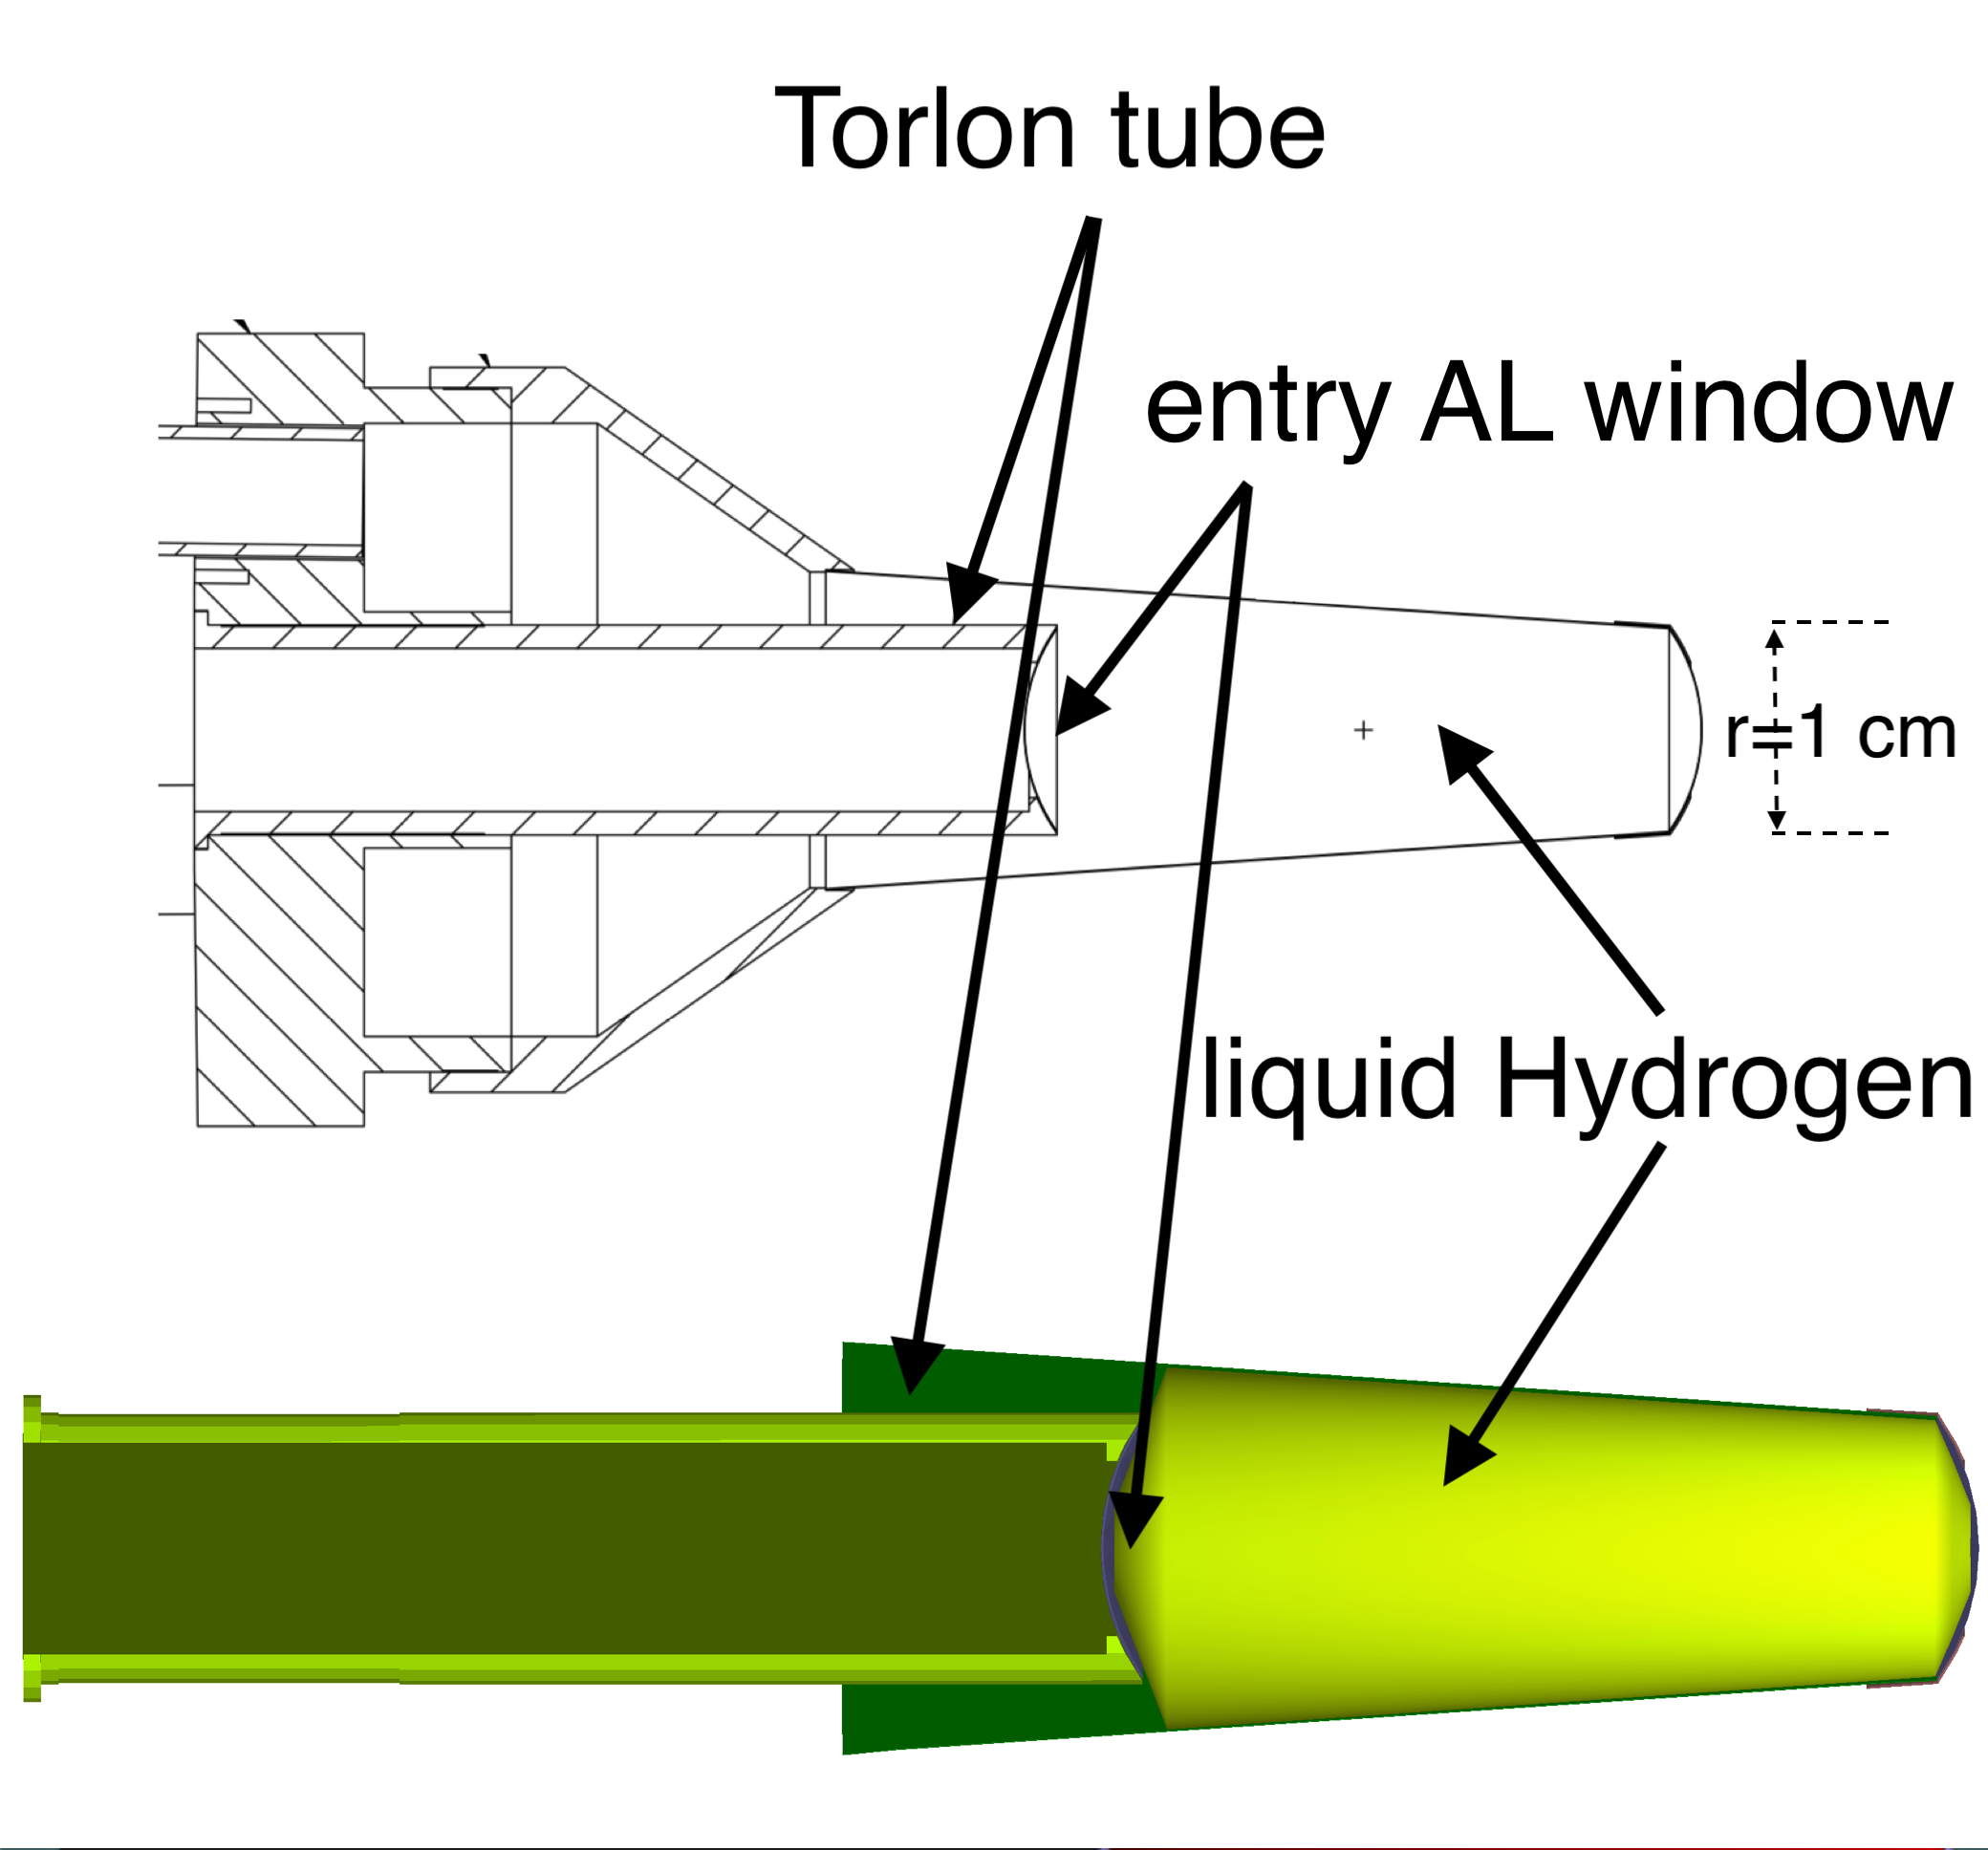
\includegraphics[width=0.95\columnwidth,keepaspectratio]{img/targetDesign.png}
	\caption{The CLAS12 target design. Top left: the entry assembly schematic. Top right: the liquid hydrogen cell
            dimensions: the outer radius is tapered down from 15 mm at z=-2.5cm to 10mm at z=2.5mm.
            Bottom left: The cell implementation in GEMC from the CAD drawings. From left to right (beam direction):
            the black torlon tube, the upstream aluminum window, the target cell, the kapton cup and the
				downstream aluminum window. Bottom right: the GEMC implementation of the kapton cup.}
	\label{fig:targetDesign}
\end{figure}


\subsubsection{Geometry Git Location}
The github location of the gemc perl api scripts and the STL files is \url{https://github.com/gemc/detectors/tree/master/clas12/targets}.






\subsection{Silicon Vertex Tracker (SVT)}


\subsubsection{Geometry}


The SVT \cite{svt-nim} geometry is implemented through a java service, the same used to provide the geometry
to the reconstruction software \cite{recon-nim}.
This service provides the Geant4 definitions that are read by the GEMC perl API to build the geometry database.

There are three SVT regions, with 10, 14, and 18 sectors/modules for Regions 1, 2, and 3, respectively, see \F{bstGeometry}.
Each module has six sensors, four readout chips as passive materials, and several material
components in the active area, listed in order below:

\begin{itemize}
	\item wirebond
	\item silicon
	\item epoxy
	\item rail
	\item bus cable
	\item carbon fiber
	\item ROHACELL
	\item carbon fiber
	\item bus cable
	\item rail
	\item epoxy
	\item silicon
	\item wirebond
\end{itemize}

The active area of the silicon sensor is associated with the SVT hit process routine.
The strip identification is performed in the Process ID routine.

\begin{figure}
	\centering
	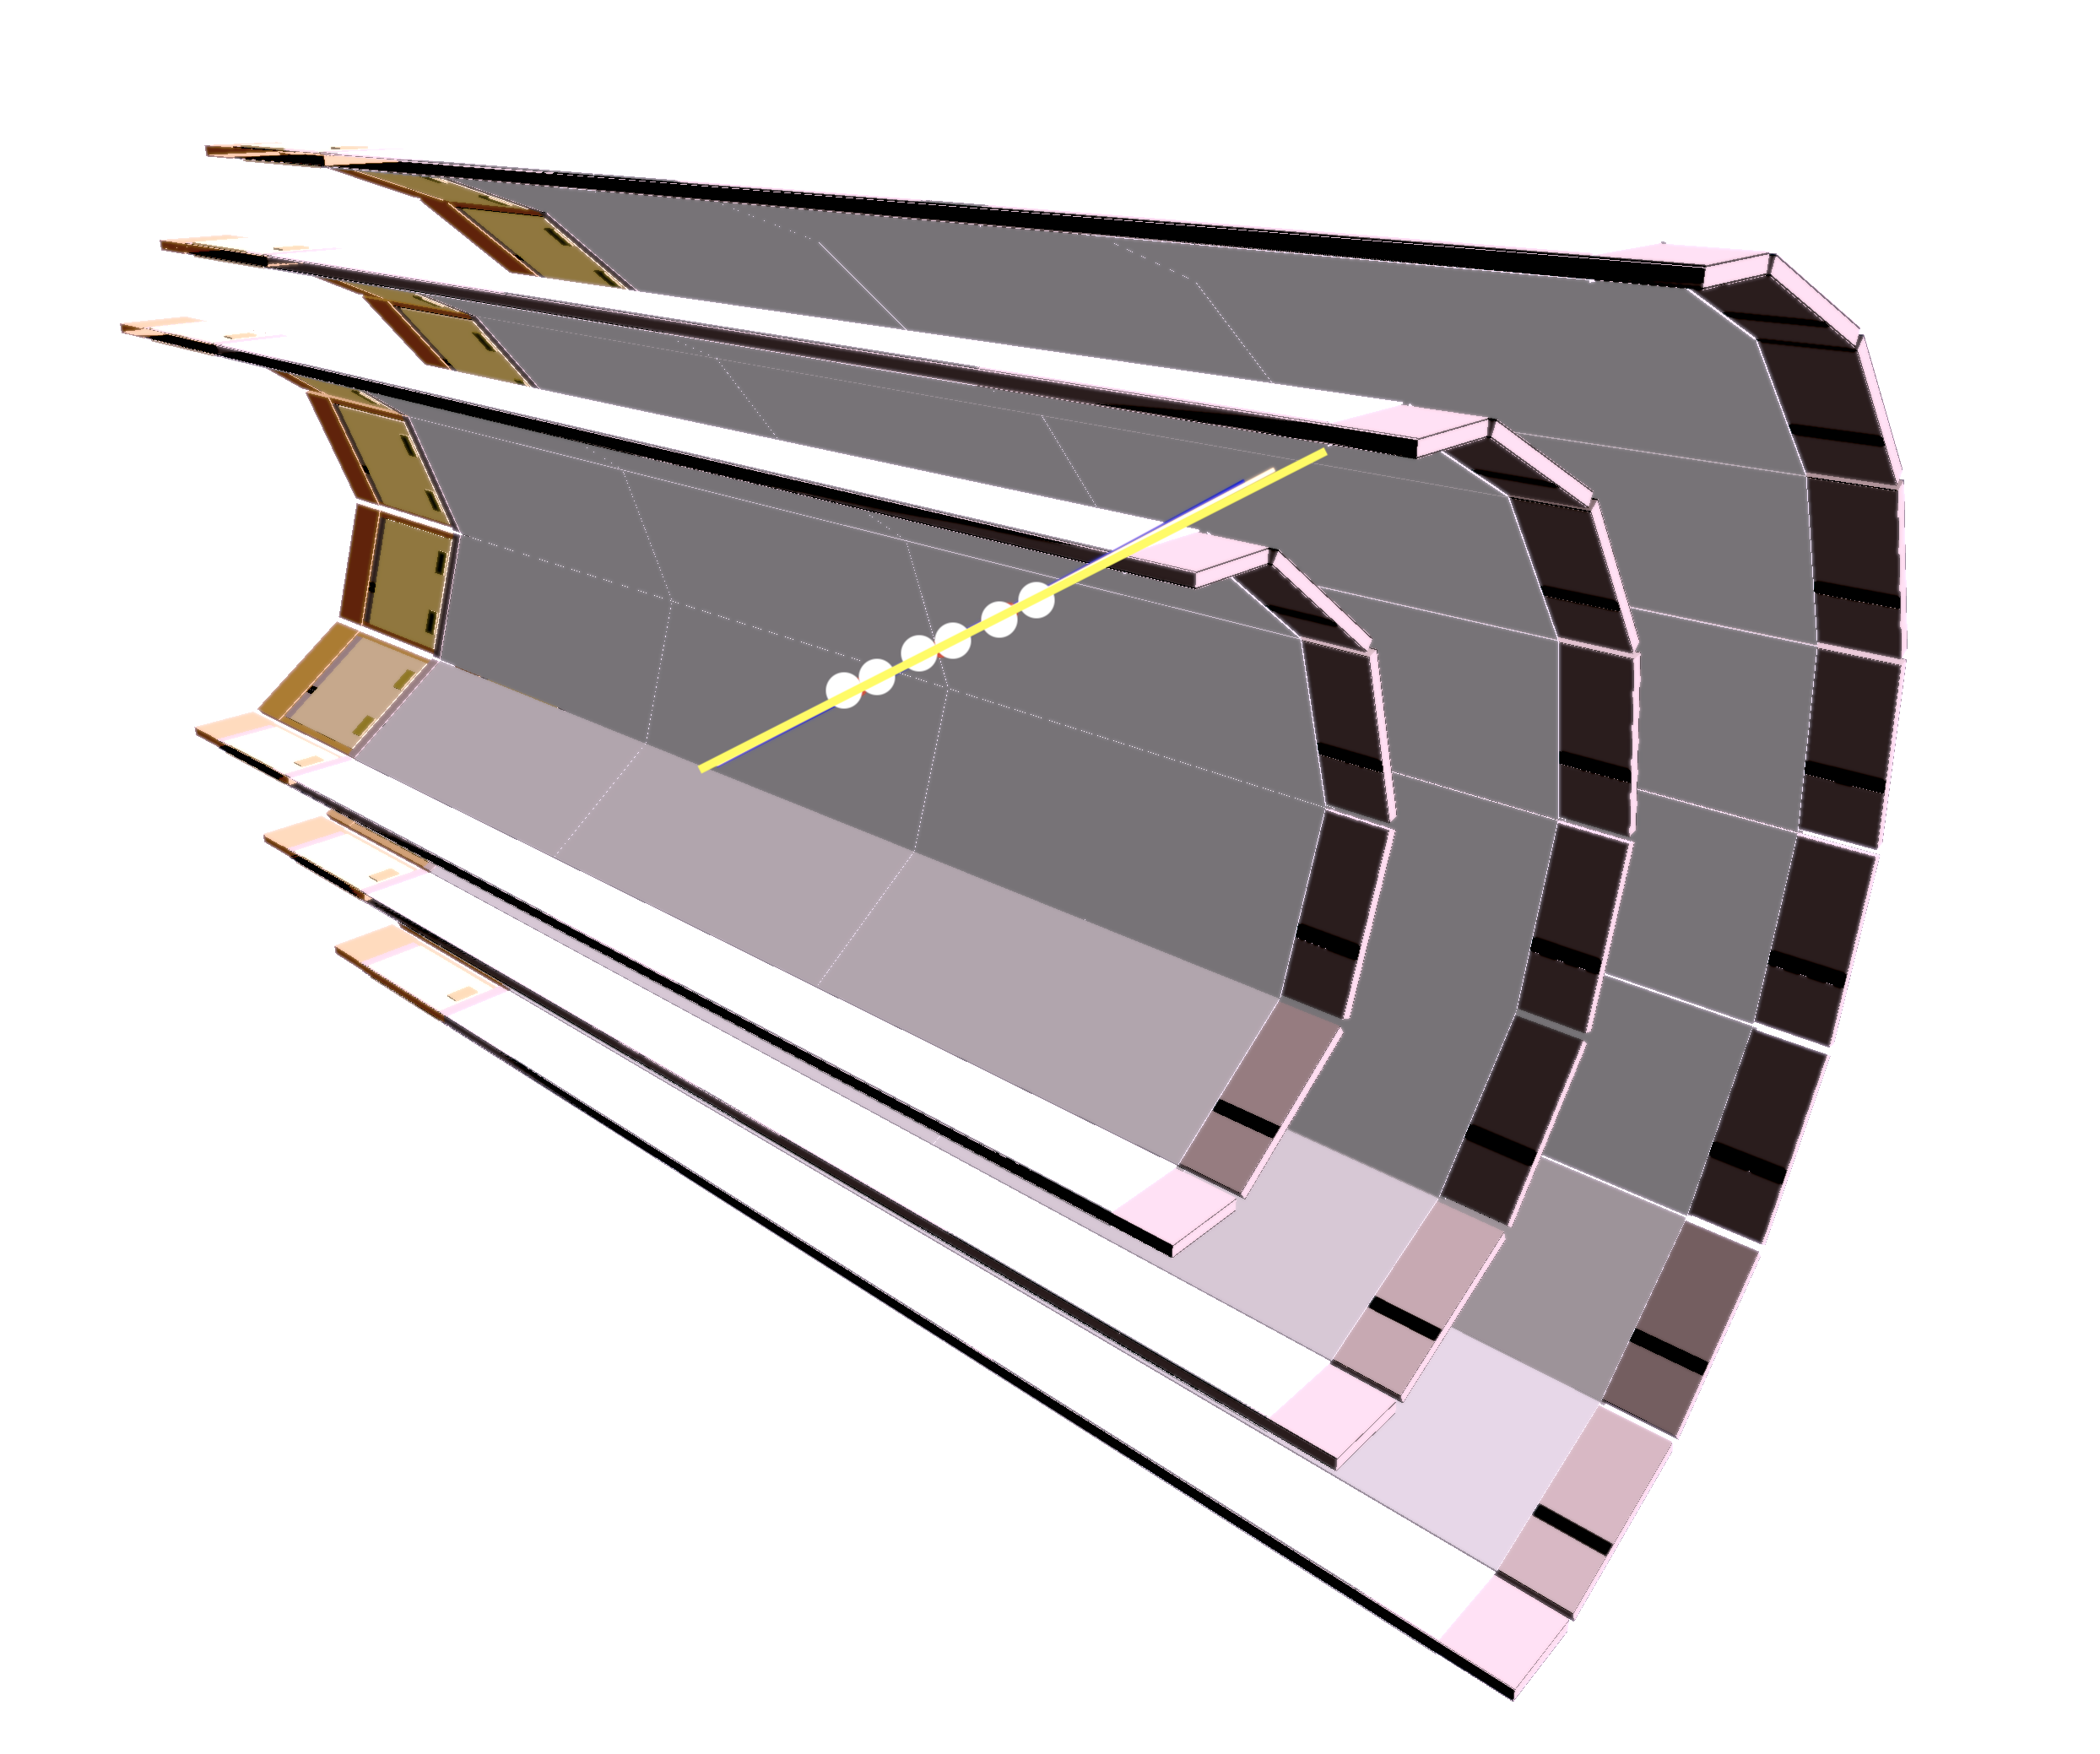
\includegraphics[width=0.99\columnwidth,keepaspectratio]{img/bstGeometry.png}
	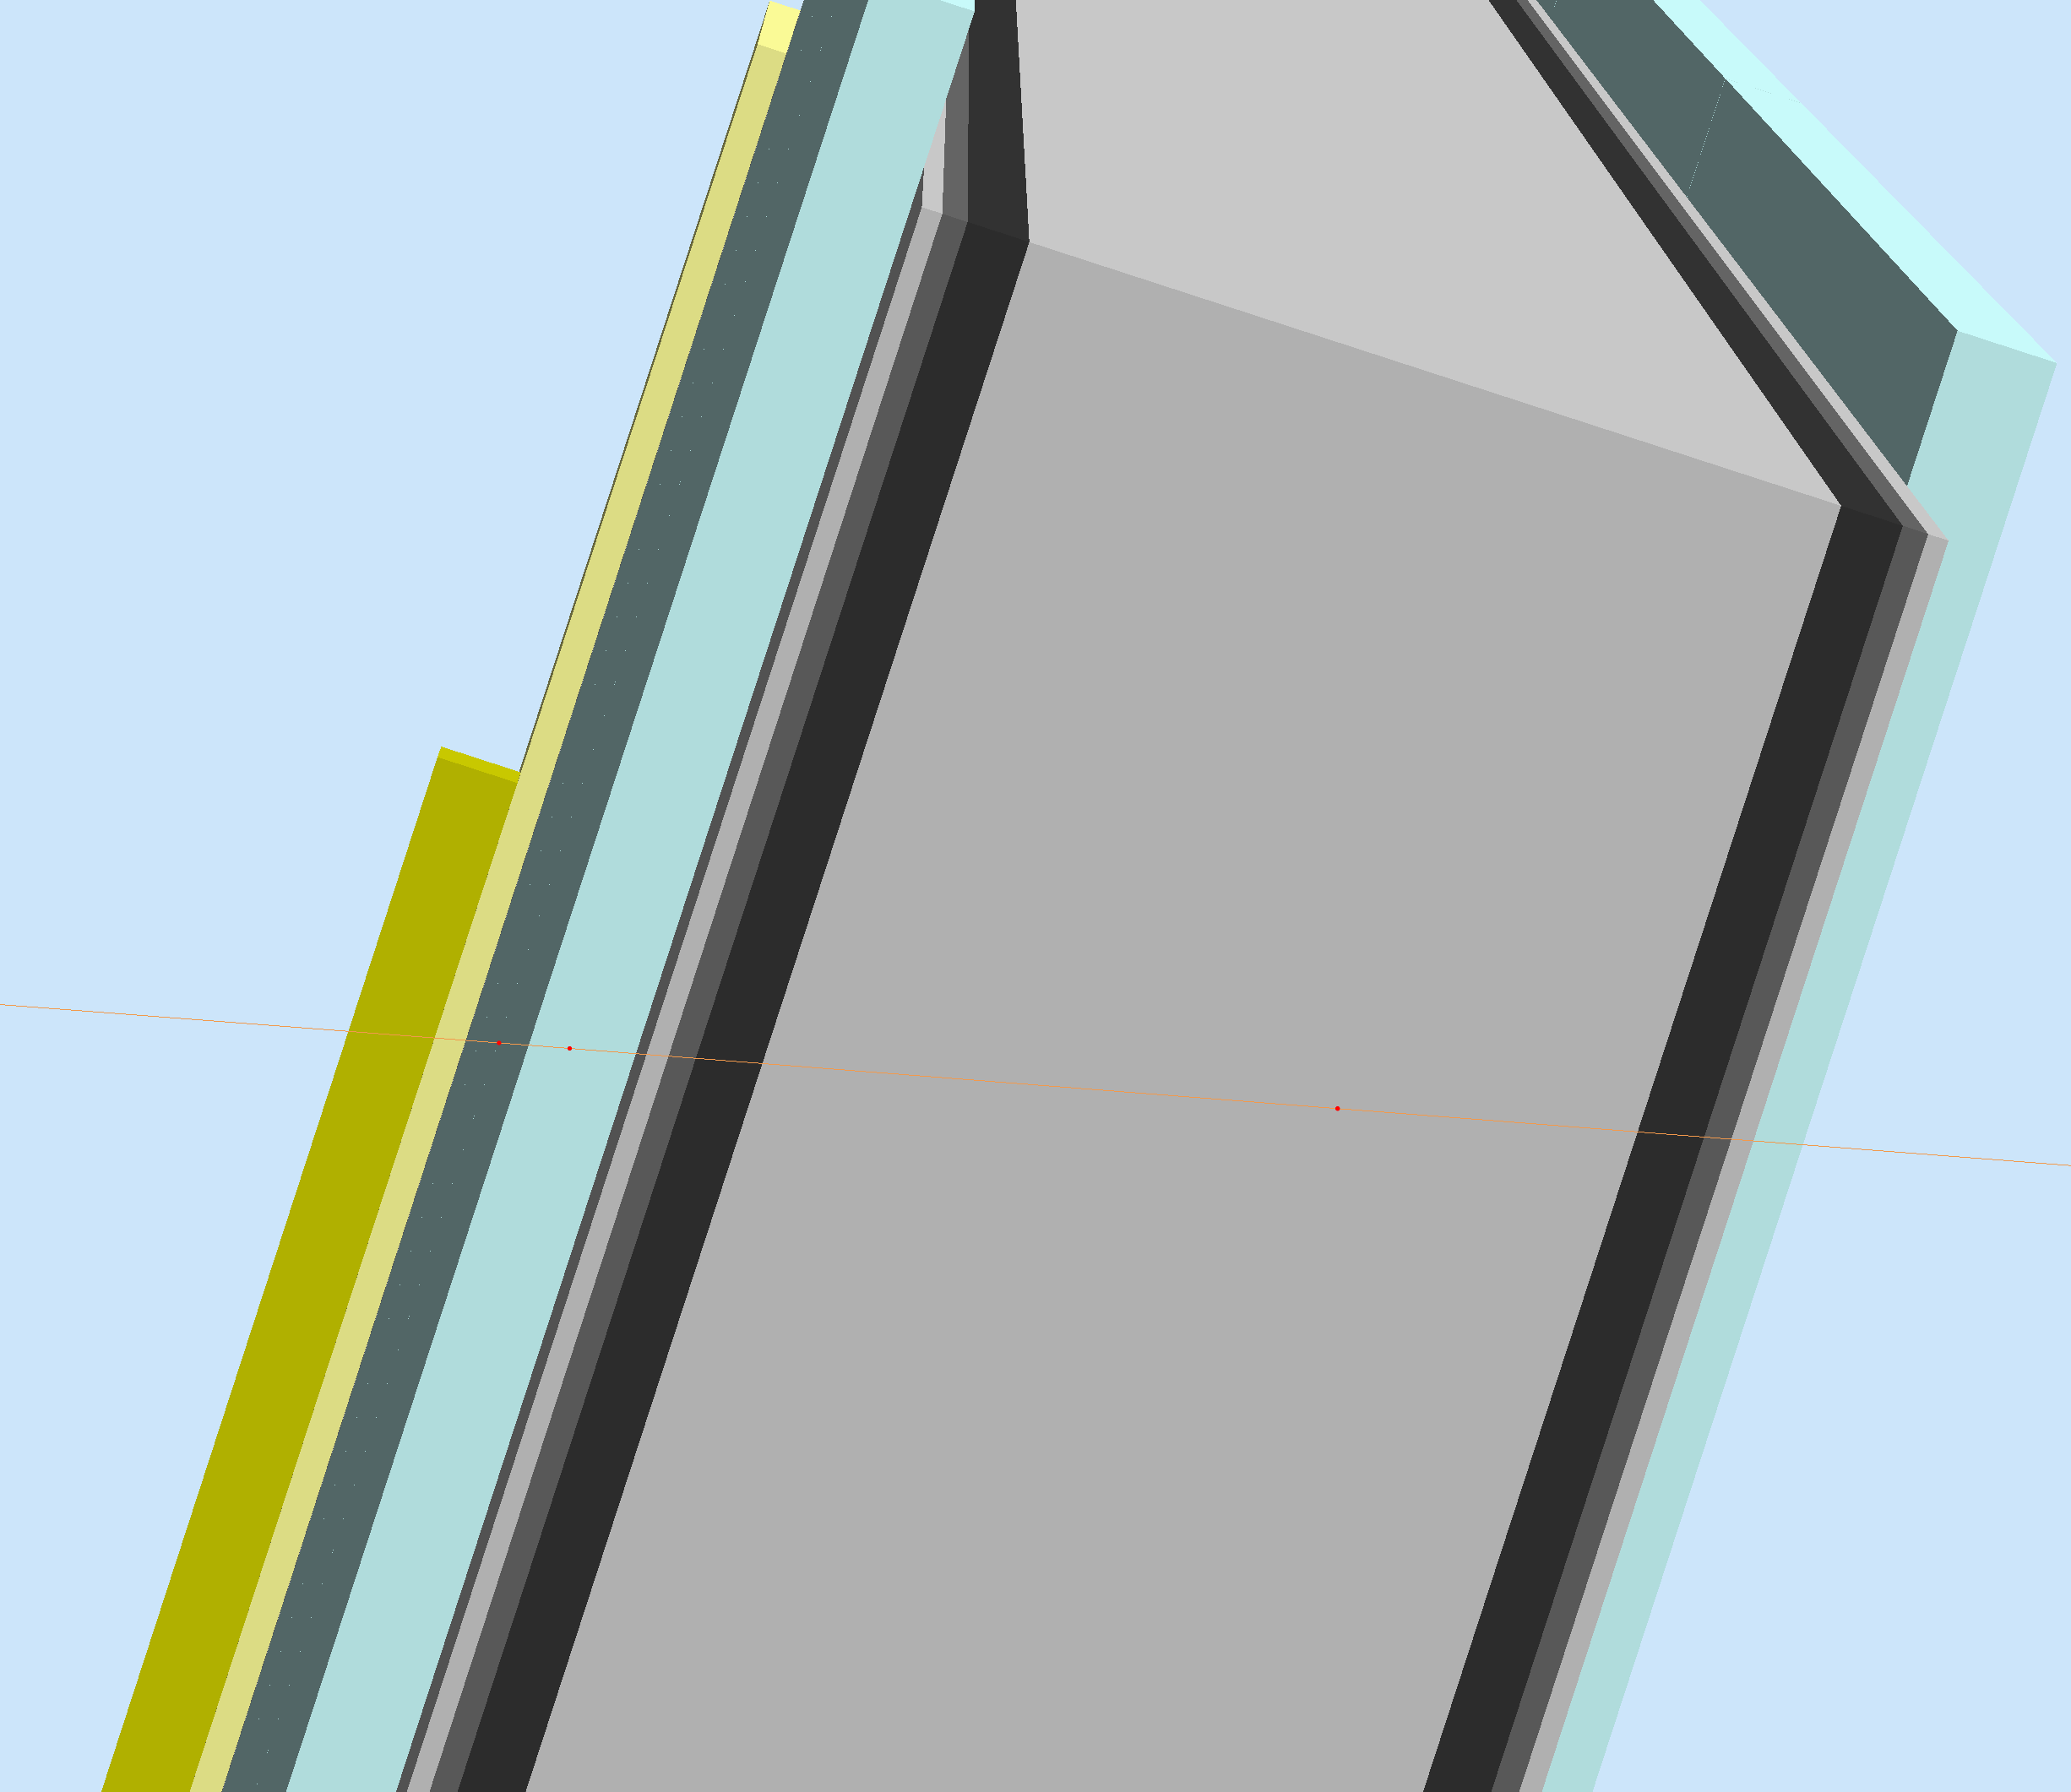
\includegraphics[width=0.99\columnwidth,keepaspectratio]{img/bstDetail.png}
	\caption{Top: the GEMC implementation of the SVT geometry (longitudinal cut-view).
	         The three regions are shown in the sliced view. The silicon sensors are
             the gray color rectangles. The track is a 2 GeV proton, leaving hits (marked with white circles)
			 in each sensor crossed. Bottom: detail of a module shows
             the various materials inside. The 320 $\mu$m silicon sensor is on inner and other surfaces of the module.
             The material inside includes epoxy glue, the bus cable, and support material. The proton creates one hit
		     in both the two silicon sensors it transverses.}
	\label{fig:bstGeometry}
\end{figure}


\subsubsection{Process ID}

At each Geant4 step, the local coordinates in the sensor volume are used to calculate the strip number.
The algorithm includes: the dead zone around the sensor, the pitch between the readout strips (156 $\mu$m), and the angle
between the strips that varies from 0\mdeg \ (for strip $\# 1$) to 3\mdeg \ (for strip  $\# 256$).
An illustration of the strip assignment is summarized in \F{processID}.

\begin{figure}
	\centering
	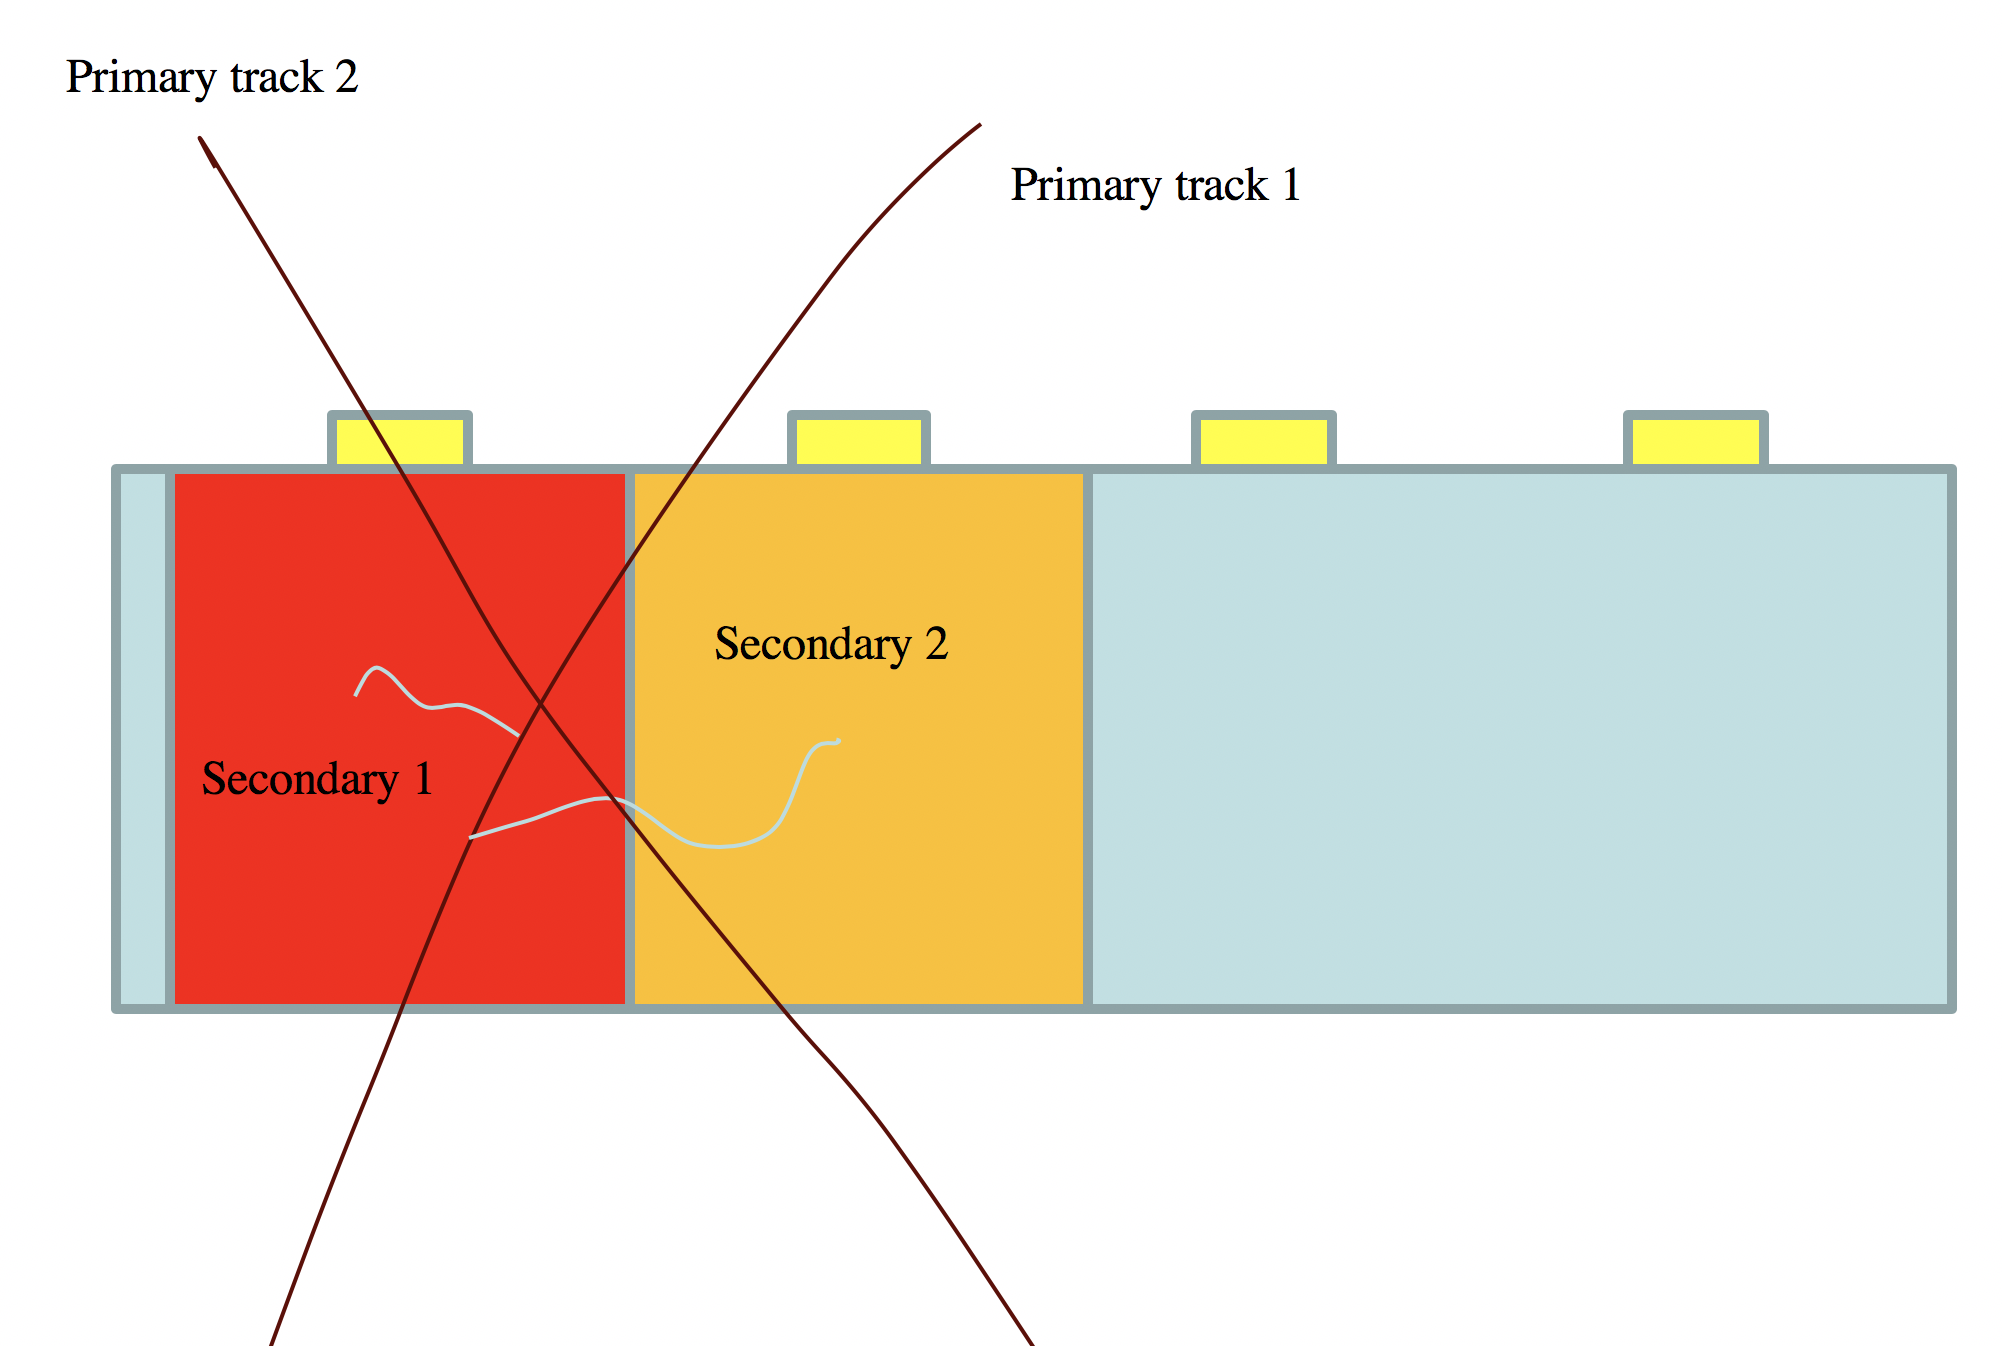
\includegraphics[width=0.99\columnwidth,keepaspectratio]{img/bstHit.png}
	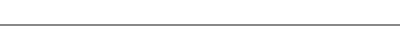
\includegraphics[width=0.99\columnwidth,keepaspectratio]{img/blank.png}
	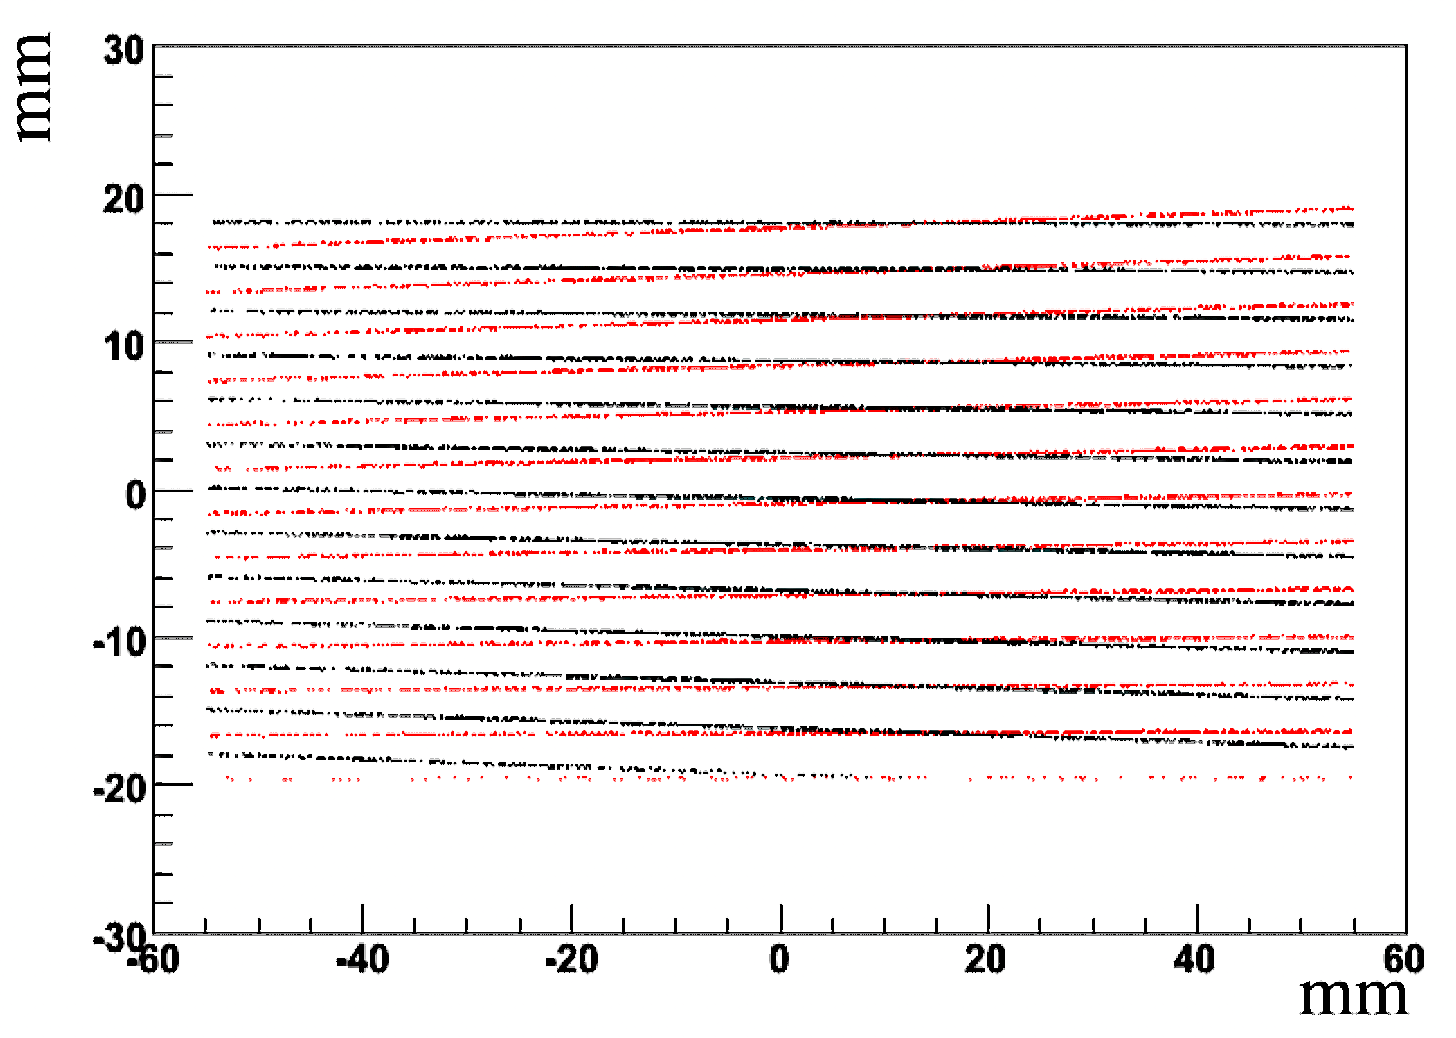
\includegraphics[width=0.99\columnwidth,keepaspectratio]{img/bstStrip.png}
	\caption{Top: Process ID algorithm cartoon for the SVT. The strip number is assigned based on the local
             position of the track step within the sensitive module.
             Bottom: the hit position of every 20th strips in the simulation outlines the strip boundaries.
             The solid and dotted distributions show the fan-like angle distributions of the strips, with opposite
             directions for the inner and outer layers. }
	\label{fig:processID}
\end{figure}

Due to the thickness of the silicon sensor, the produced electron avalanche can end up in more than one strip. This
is reproduced in the GEMC simulation using the hit sharing algorithm described in \F{bstHitSharing}.

\begin{figure}[t]
	\centering
	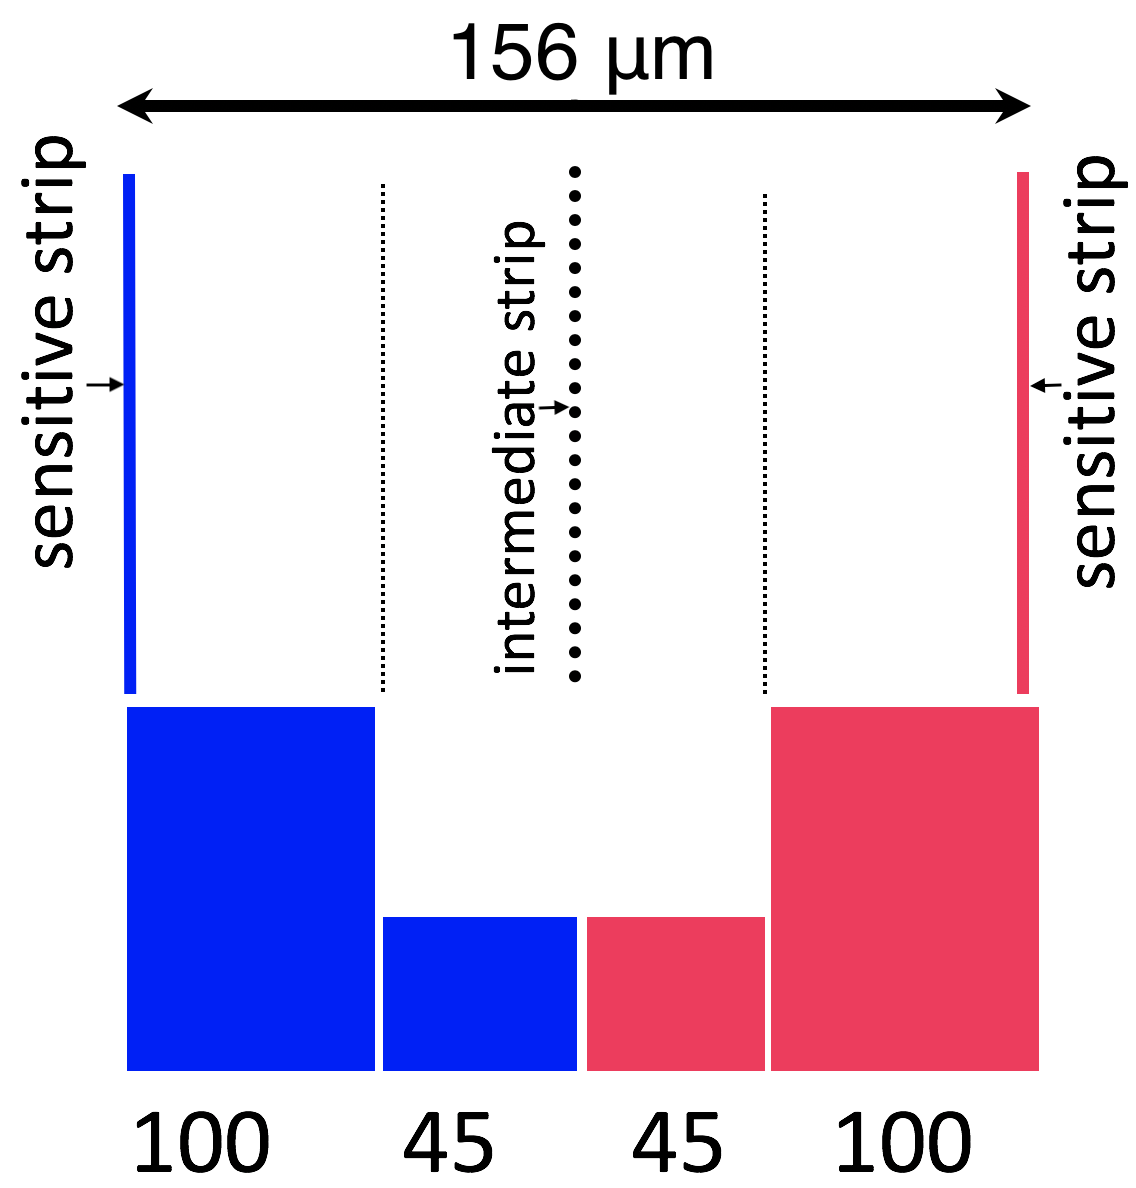
\includegraphics[width=0.99\columnwidth, keepaspectratio]{img/bstHitSharing.png}
	\caption{The SVT hit sharing algorithm. The intermediate strip represent a space between two adjacent strips
             used in the BST hit digitization algorithm. If a step happens inside the intermediate strip
             then $90\%$ of the its energy will be shared equally between the left and right strips (45$\%$ each),
             with a 10$\%$ energy loss due to capacity coupling between the strip and the back-plane.}
	\label{fig:bstHitSharing}
\end{figure}


\subsubsection{Digitization}

The SVT digitization provides a 3-bit ADC, using the total energy deposited (after hit sharing) between 26 and 117 keV.
The Bunch Cross Oscillator quantity (BCO), a random number between 0 and 255,
provides the TDC timing information associated with the hit.
The digitized output bank variables are summarized in Table \ref{tab:bstBank}.

\begin{table}[h]
	\begin{center}
		\begin{tabular}{| c | c | c |}
			\hline \hline
			Variable  & Description   \\
			\hline
               layer  &        layer number    \\
              sector  &       sector number    \\
               strip  &        strip number    \\
                 ADC  &           3 bit ADC    \\
                 bco  &     8 bit time info    \\
               ADCHD  &          13 bit ADC    \\
                hitn  &          hit number    \\
			\hline \hline
		\end{tabular}
	\end{center}
	\caption{The digitized SVT bank.}\label{tab:bstBank}
\end{table}

The time window  of the SVT is set to to 128 ns: all Geant4 steps within the same strip and time window are collected in one hit.

\subsubsection{Radiation Dose and Background Rates}
A detailed study of the background rates coming from beam interacting with the target was done to ensure that the silicon sensor
could operate in the high radiation conditions of the target proximity.
Given the nominal operating luminosity L=\cLuminosity, and the liquid-hydrogen target of 5 cm length, the beam electron rate
is $R=4.7 \times 10^{11} Hz$. This corresponds to about 62,000 electrons in the 128 ns SVT time window.

Simulations using 62,000 11 GeV electrons per event impinging on the liquid-hydrogen target were analyzed.
The rates were calculated for the various regions and for different thresholds (see \F{radStudyThreshold}).
The radiation dose and the 1 MeV neutron equivalent damage was estimated. Most of the radiation
is released in the first two layers of the SVT.
The 370 rad/year is low enough for an operating lifetime of at least 15 years. The results of the study
are summarized in \F{radStudy}.


\begin{figure}
	\centering
	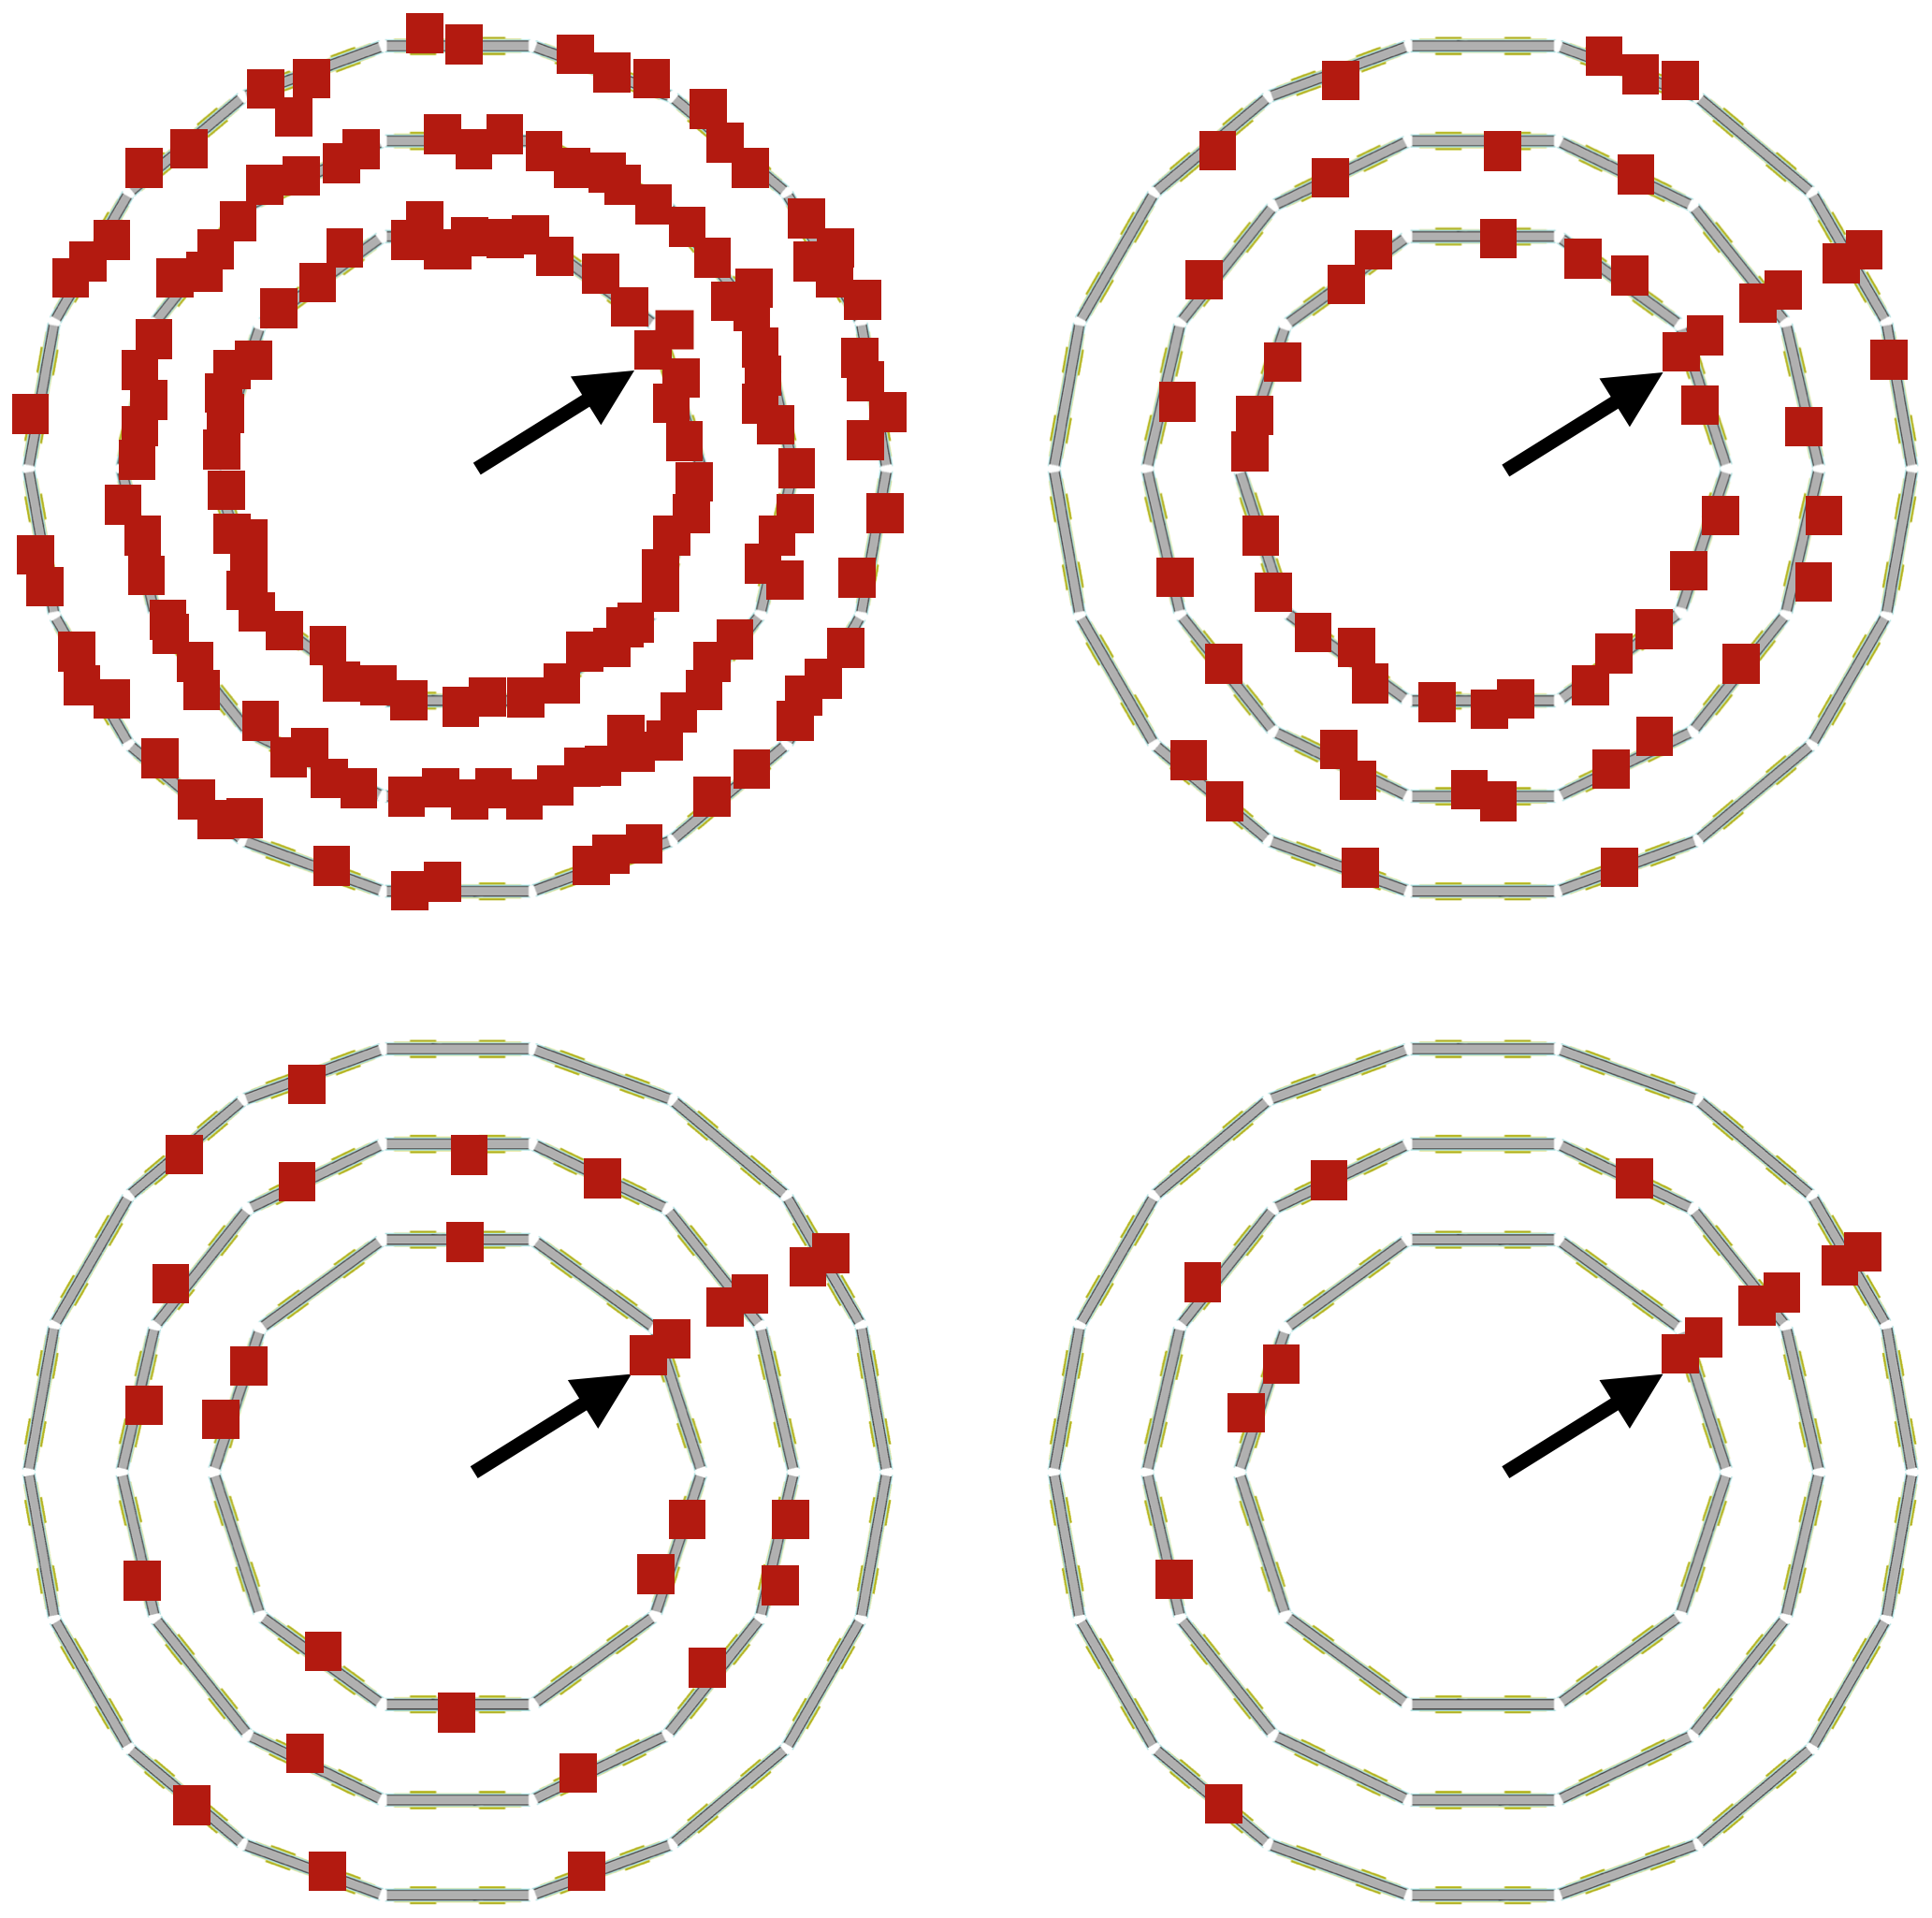
\includegraphics[width=0.99\columnwidth,keepaspectratio]{img/bstHitDisplay.png}
	\caption{The occupancy in the various SVT layers for different thresholds for one event containing a proton
             track (direction indicated by the arrow). The hits are represented by the square.
             Top left: with no energy cut, all SVT layers have numerous hits. Top right: a 10 keV energy threshold
             reduces the SVT occupancy considerably. Most ($>90\%$) of the hits removed come from photons.
             Bottom left: 20 keV energy threshold. Bottom right: 30 keV energy threshold.
             The SVT final choice of threshold, based on background rejection study, was 30 keV. }
	\label{fig:radStudyThreshold}
\end{figure}




\begin{figure}
	\centering
	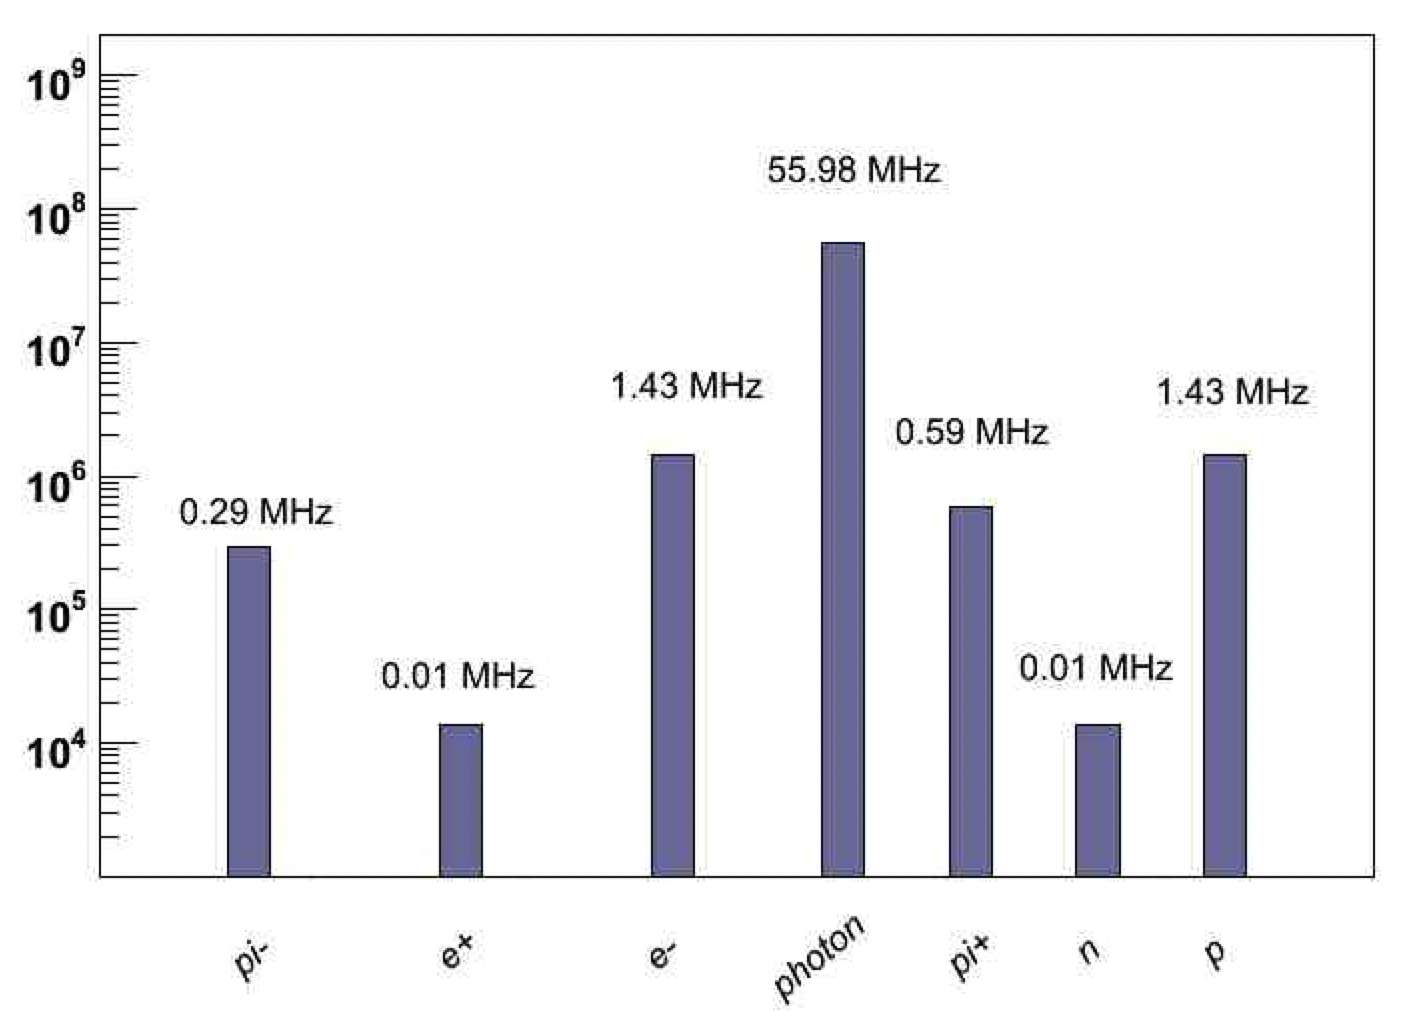
\includegraphics[width=0.99\columnwidth,keepaspectratio]{img/bstRates.png}
	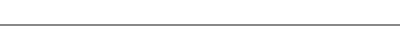
\includegraphics[width=0.99\columnwidth,keepaspectratio]{img/blank.png}
	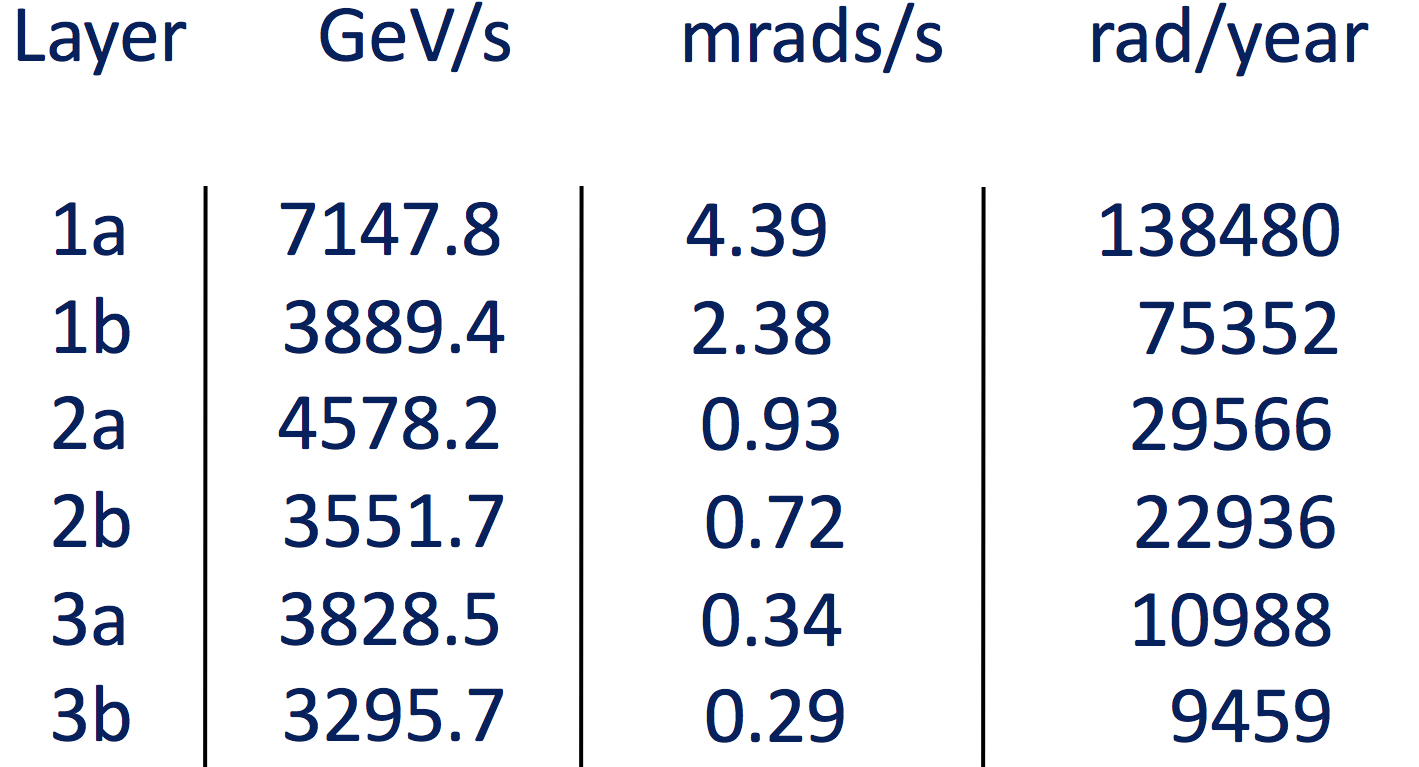
\includegraphics[width=0.99\columnwidth,keepaspectratio]{img/bstRadSummary.png}
	\caption{Summary of radiation doses and background rates in the SVT. Top: the rate breakdown for different particles
             for a threshold of 20 keV (the current hardware threshold is 30 keV) at the full luminosity of CLAS12.
             Bottom: table showing the fluences and radiation doses in the SVT layers. }
	\label{fig:radStudy}
\end{figure}

Based on these GEMC background studies in conjunction with SVT studies with beam, a thin layer of tungsten
(51 $\mu$m) was added between the target and the inner SVT layer aimed at reducing the electromagnetic
background \cite{bstDose}.






\subsection{Barrel Micromegas Tracker (BMT)}

\subsubsection{Geometry}

The Micromegas geometry is implemented through the native GEMC geometry API.
There are three micromegas regions, divided azimuthally in three identical sectors. Each sector contain a cover layer with copper ground,
the PCB with the readout strips, the Kapton support, the mesh layer, the ionizing gas, and other layers of material, listed in order below:

\begin{itemize}
	\item overlay
	\item copper ground
	\item PCB
	\item strips
	\item Kapton
	\item gas (amplification gap)
	\item mesh
	\item gas (drift detection gap)
	\item drift potential electrode
	\item foil
	\item ground
\end{itemize}

The sensitive volume contains argon isobutane gas and is associated with the BMT hit process routine.
The geometry is summarized in \F{bmtGeometry}. The strip IDentification is performed in the Process ID routine.

\begin{figure}
	\centering
	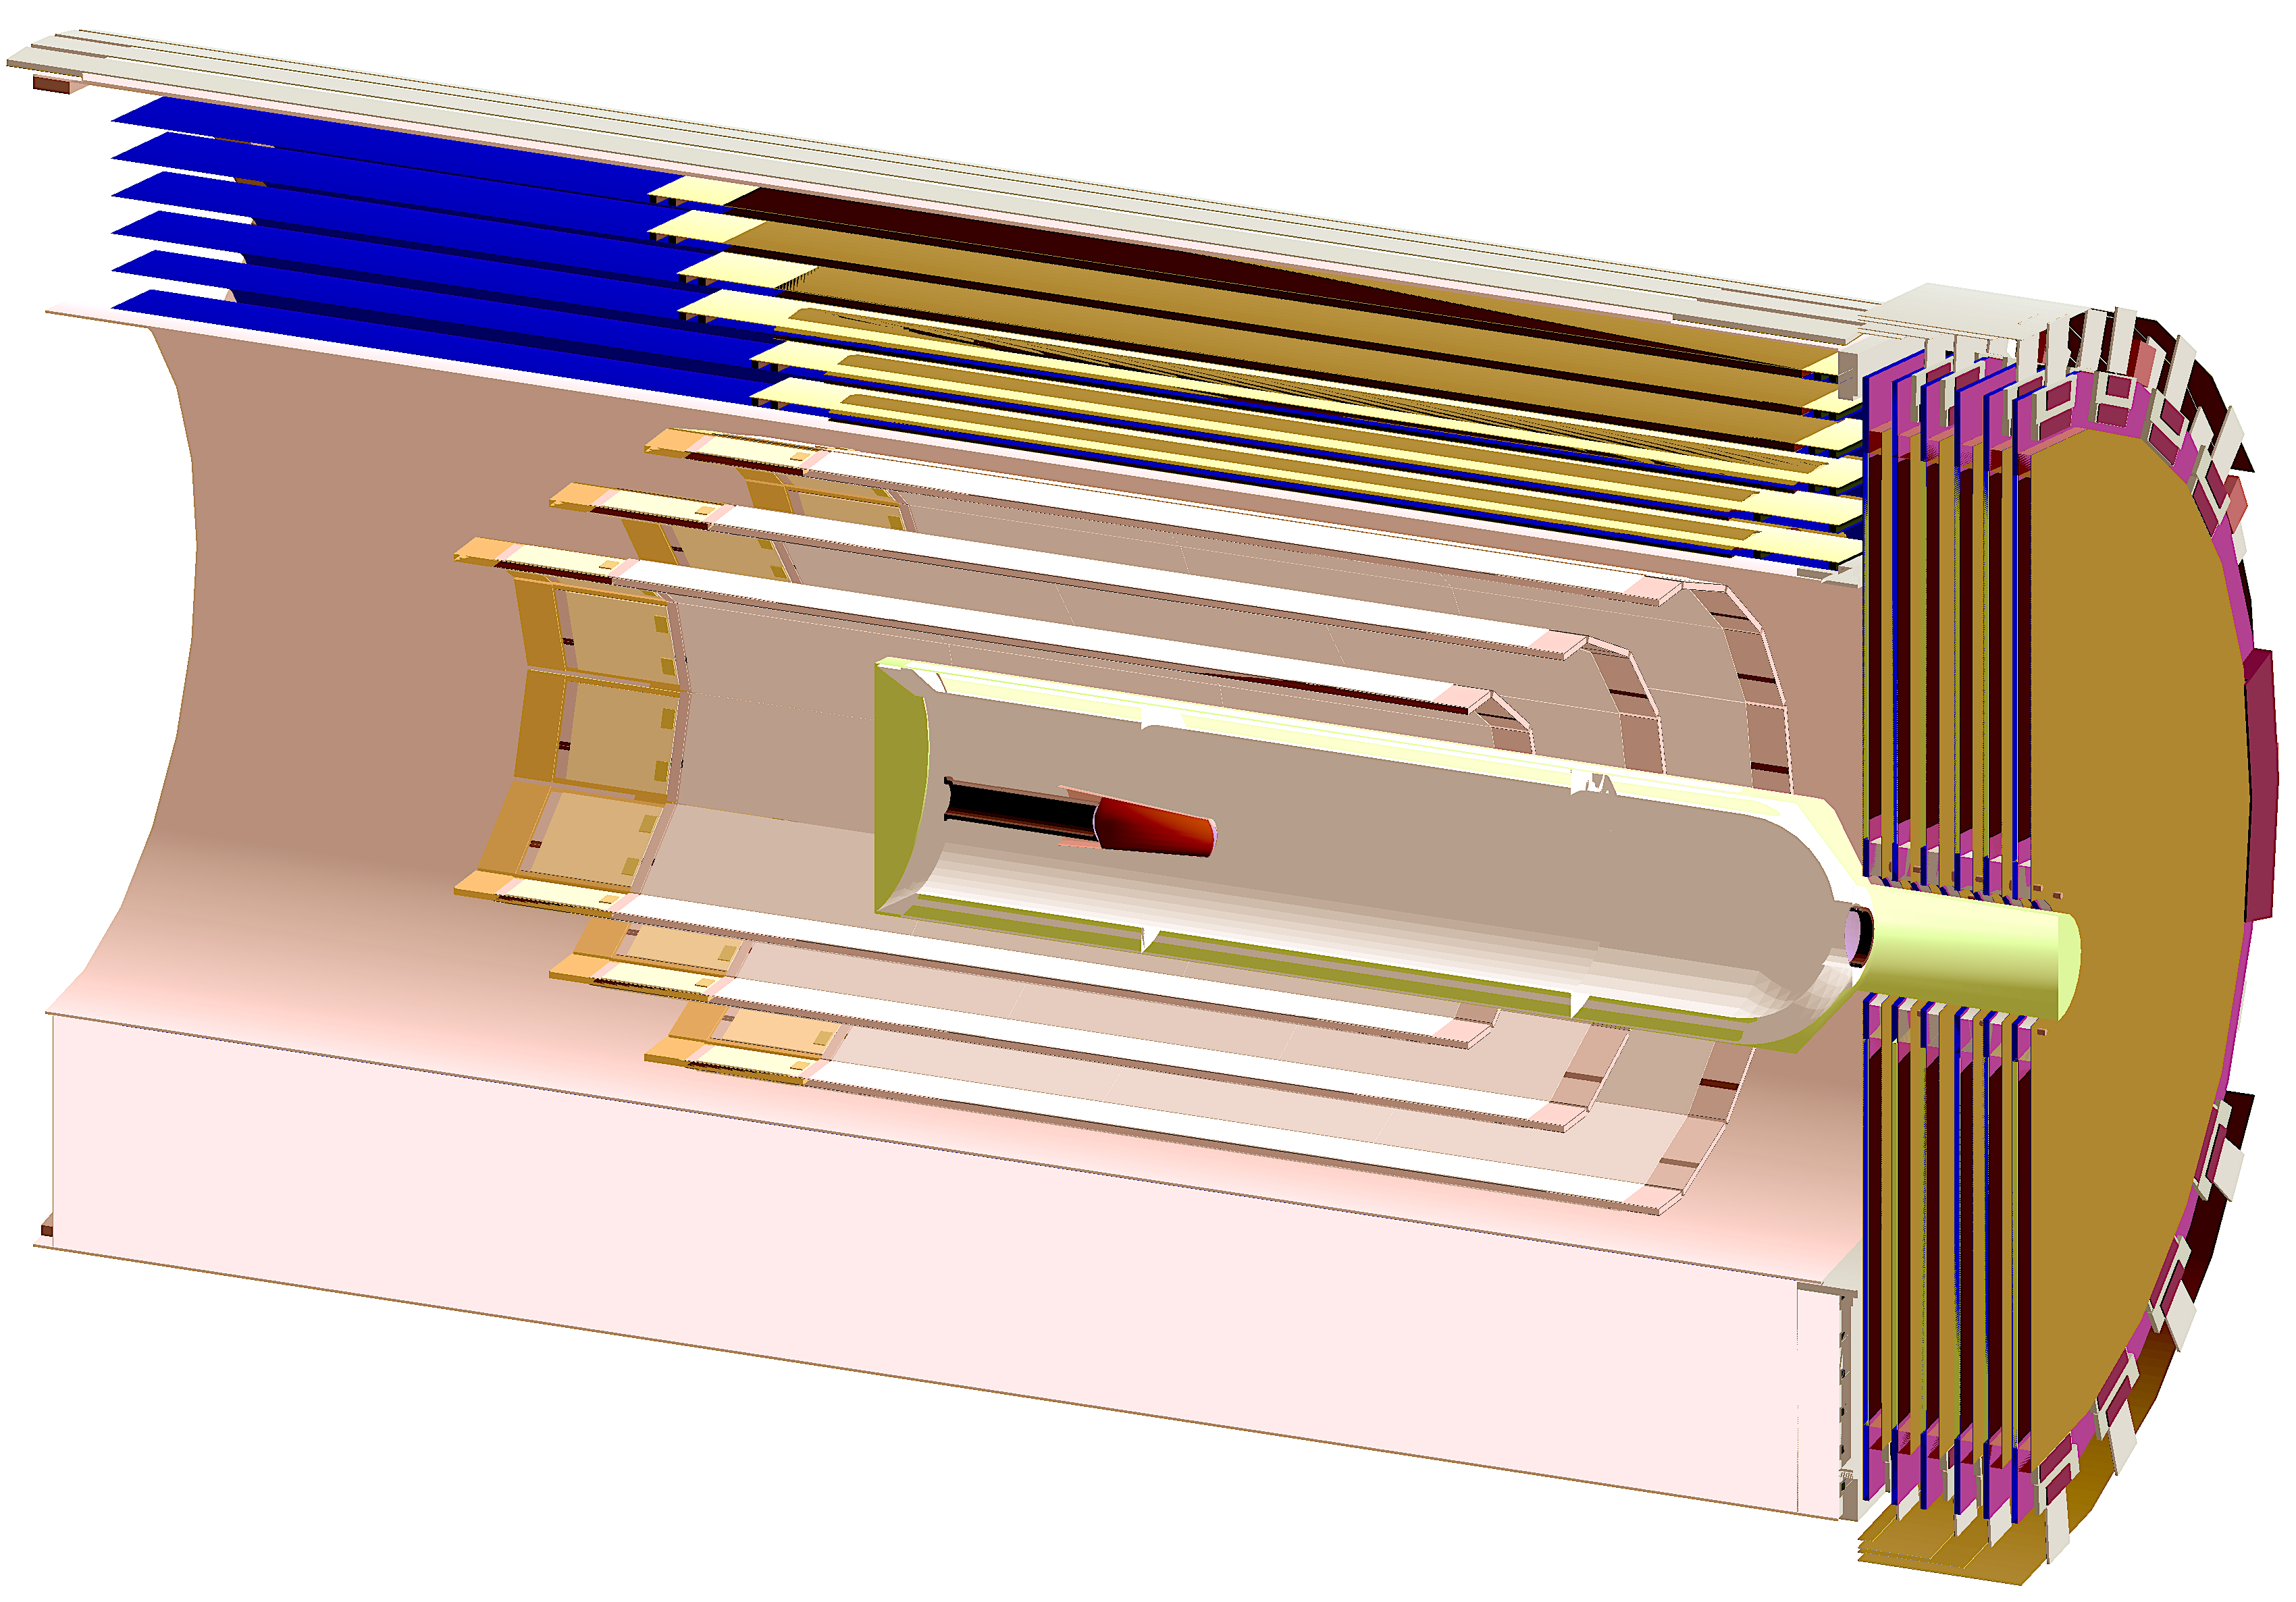
\includegraphics[width=0.99\columnwidth,keepaspectratio]{img/bmtGeometry.png}
	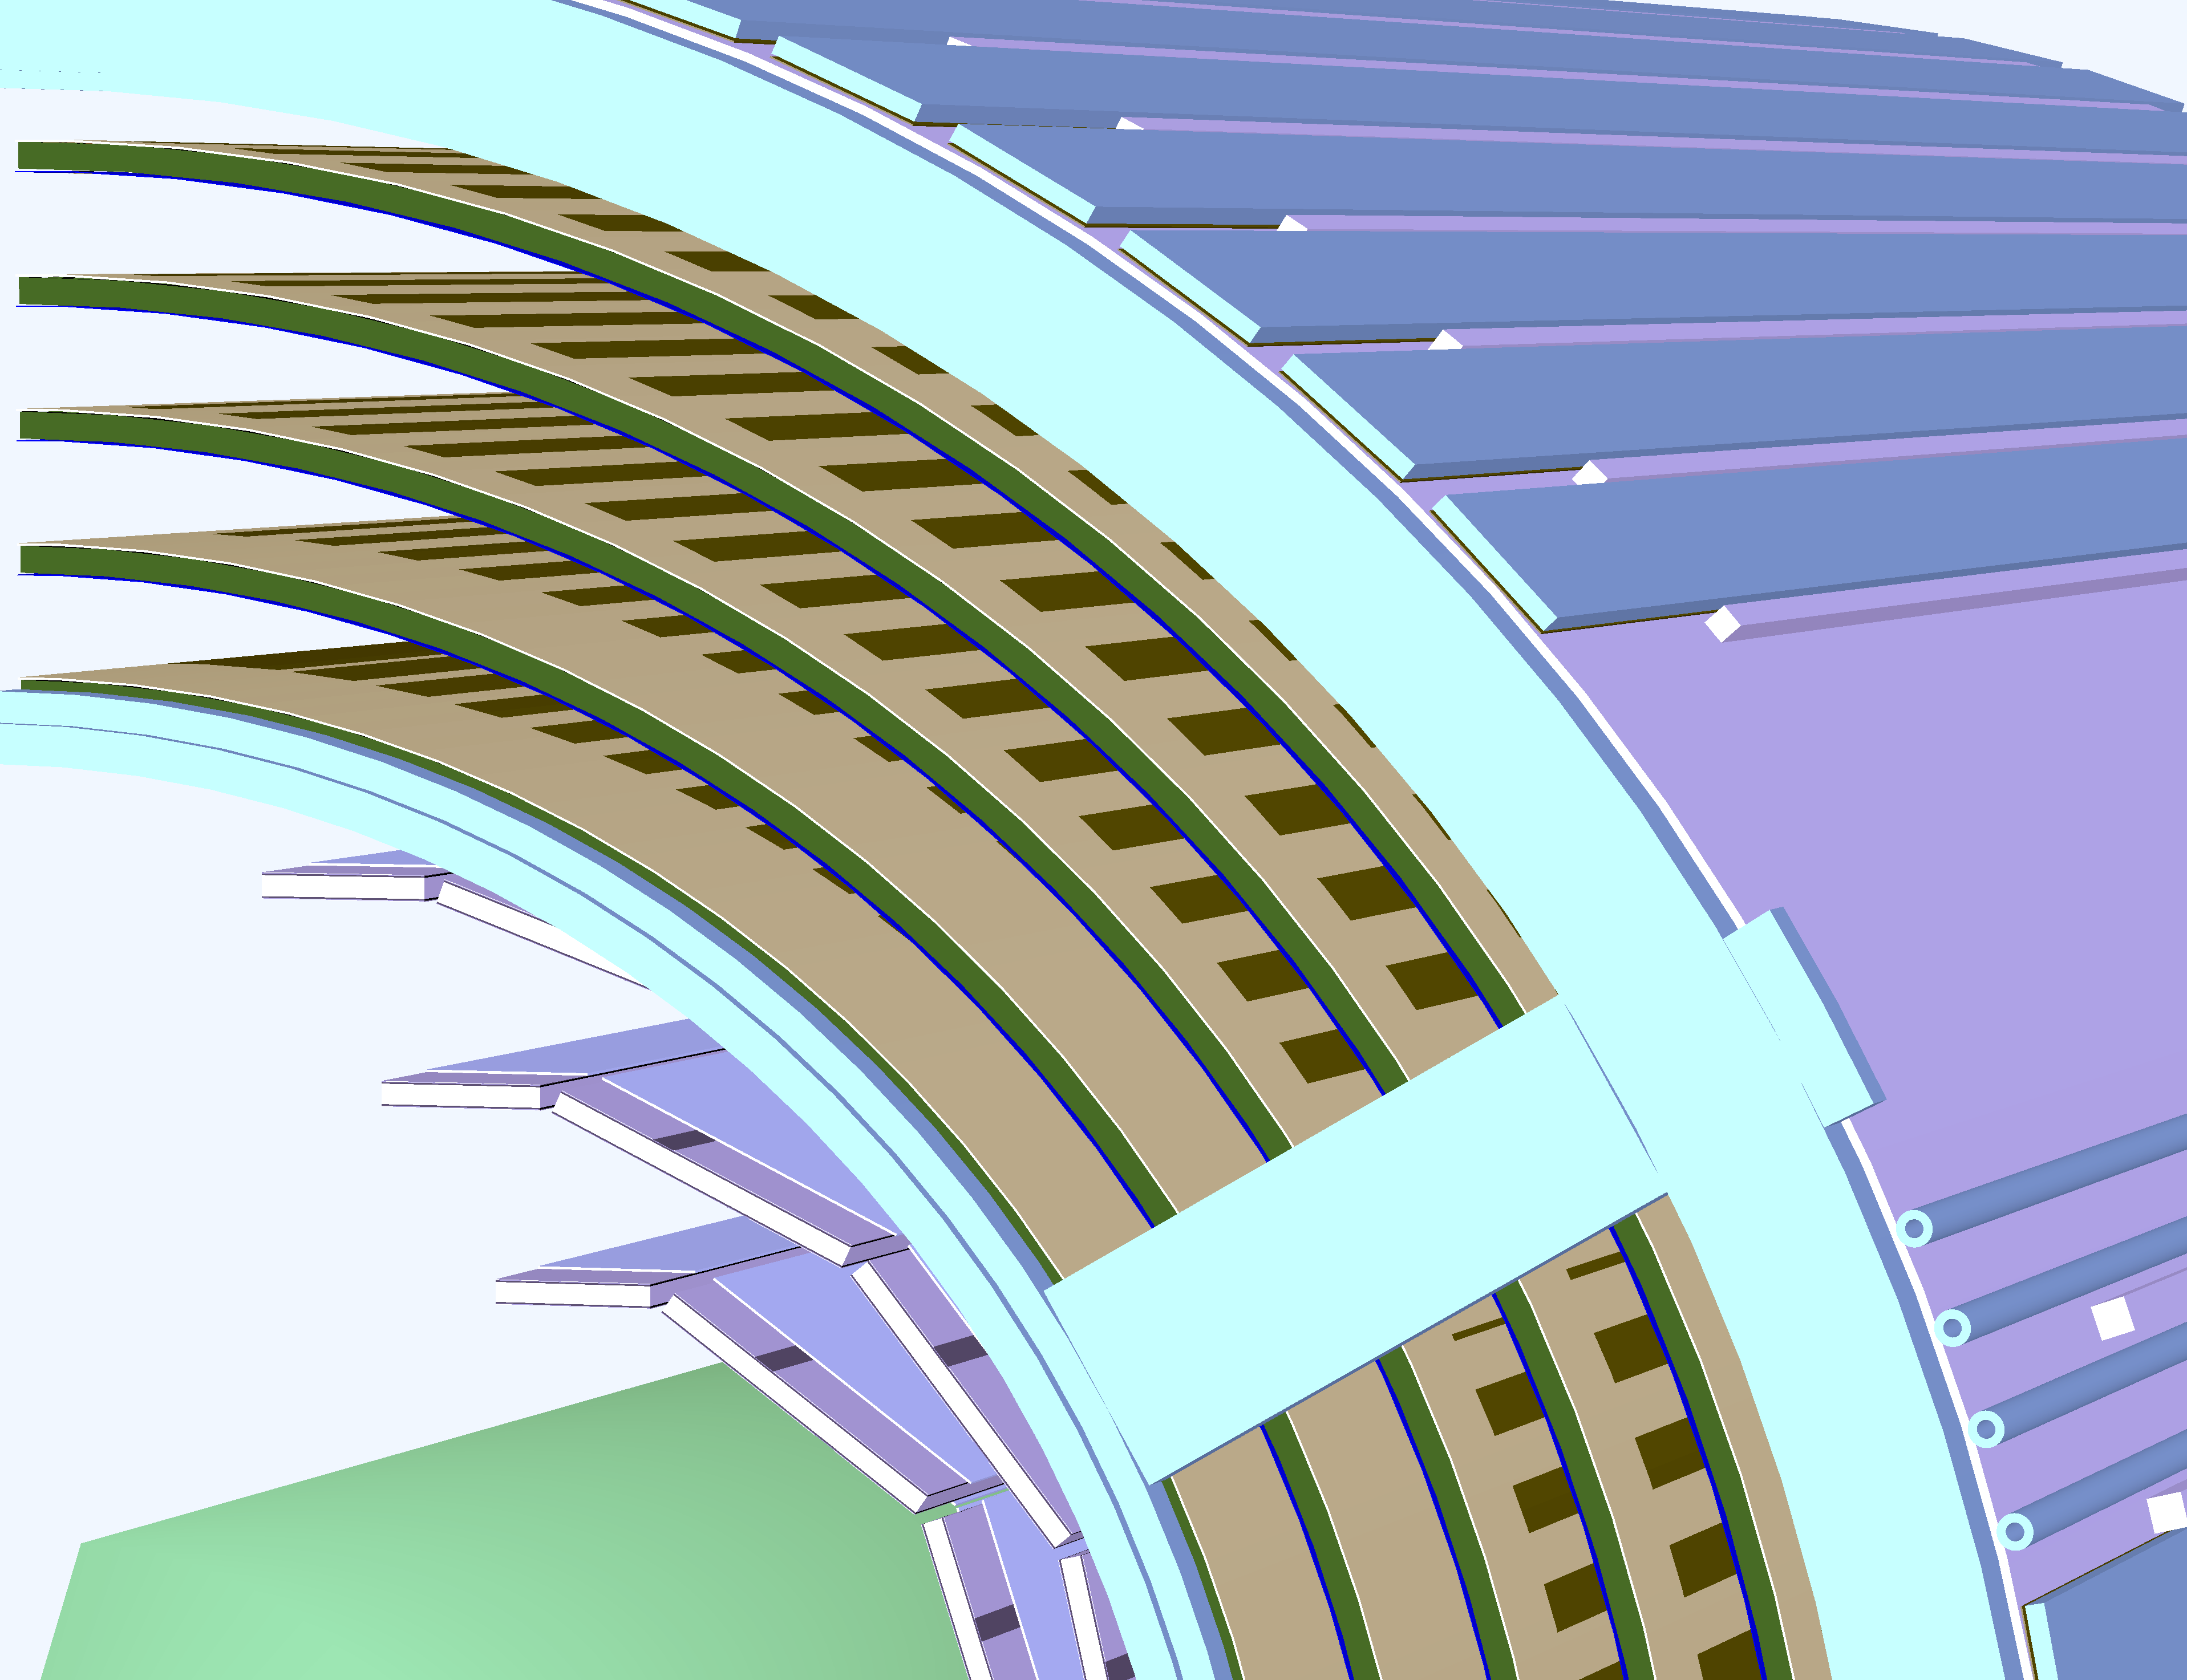
\includegraphics[width=0.99\columnwidth,keepaspectratio]{img/bmtDetail.png}
	\caption{Top: an overall view of the CLAS12 Central Detector trackers. The target is surrounded by 3 layers of SVT and
            6 layers of micromegas, 3 with ```Z'''-strips, 3 with ```C'''-strips. On the front the Forward Micromega Tracker disks are visible.
            Bottom: detail of the micromegas GEMC geometry, showing the overlay cover, the copper ground, and the PCB.}
	\label{fig:bmtGeometry}
\end{figure}

The Github location of the GEMC perl API script is \url{https://github.com/gemc/detectors/tree/master/clas12/micromegas}.


\subsection{Process ID}
At each Geant4 step, the local coordinates in the sensor volume are used to calculate the strip ID.
The algorithm includes the Lorentz angle based on the magnetic field strength, the particle direction,
the pitch angle between the strips, and the dead zones of the sensitive parts.
A virtual electron avalanche is simulated based on the energy deposited. The avalanche
is deposited onto one strip or distributed among several to account for the energy sharing.



\subsection{Digitization}

The Micromegas digitization provides the ADC value calculated using the total energy deposited (after hit sharing).
There is no timing information in the output.
The digitized output bank variables are summarized in Table \ref{tab:mmBank}.

\begin{table}[h]
	\begin{center}
		\begin{tabular}{| c | c | c |}
			\hline \hline
			Variable & Description  \\
			\hline
              layer  &      layer number   \\
             sector  &     sector number   \\
              strip  &      strip number   \\
               Edep  &  energy deposited   \\
                ADC  &               ADC   \\
			\hline \hline
		\end{tabular}
	\end{center}
	\caption{The digitized BMT bank.}\label{tab:mmBank}
\end{table}

The time window  of the Micromegas is set to to 132 ns: all geant4 steps within the same strip and time window will be collected on one hit.

The BST hit process routine location in git is \url{https://github.com/gemc/source/tree/master/hitprocess/clas12/micromegas}


\section{Central Time-Of-Flight (CTOF)}


\subsection{Geometry}

\subsection{Calibration Constants}


\subsection{Digitization}

\subsubsection{Time Window}


\section{Central Neutron Detector (CND)}


The CLAS12 CND geometry is created using the native gemc geometry API.
The geometry directory is "cnd"

\subsection{Geometry}

\subsubsection{Geometry Git Location}

\subsection{Process ID}

\subsection{Digitization}

\subsubsection{Summary of CCDB Table used}

\subsection{Digitized Bank}

\subsubsection{Time Window}

\subsubsection{Process Routine Git Repository Location}



\section{High Threshold Cerenkov Counter (HTCC)}

The CLAS12 HTCC geometry is created using the native gemc geometry API.
The geometry directory is "micromegas"


\subsection{Geometry}

\subsubsection{Geometry Git Location}

\subsection{Calibration Constants}

\subsubsection{Summary of CCDB Table used}

\subsection{Digitization}

\subsection{Process ID}

\subsubsection{Time Window}

\subsubsection{Process Routine Git Repository Location}



\subsection{Forward Tagger (FT)}


\subsubsection{Geometry}

The FT consists of three subsystems:

\begin{itemize}
	\item a micromegas tracker (FT-TRK);
	\item a hodoscope (FT-HODO);
 	\item a calorimeter (FT-CAL).
\end{itemize}

The three subsystems are implemented in GEMC using the native perl API script, except for the inner shield (see Section \ref{sec:beamline}),
which comes from the CAD engineering model.
The FT geometry is shown in \F{ftGeometry}.

\subsubsection{Digitization}

\begin{figure}
	\centering
	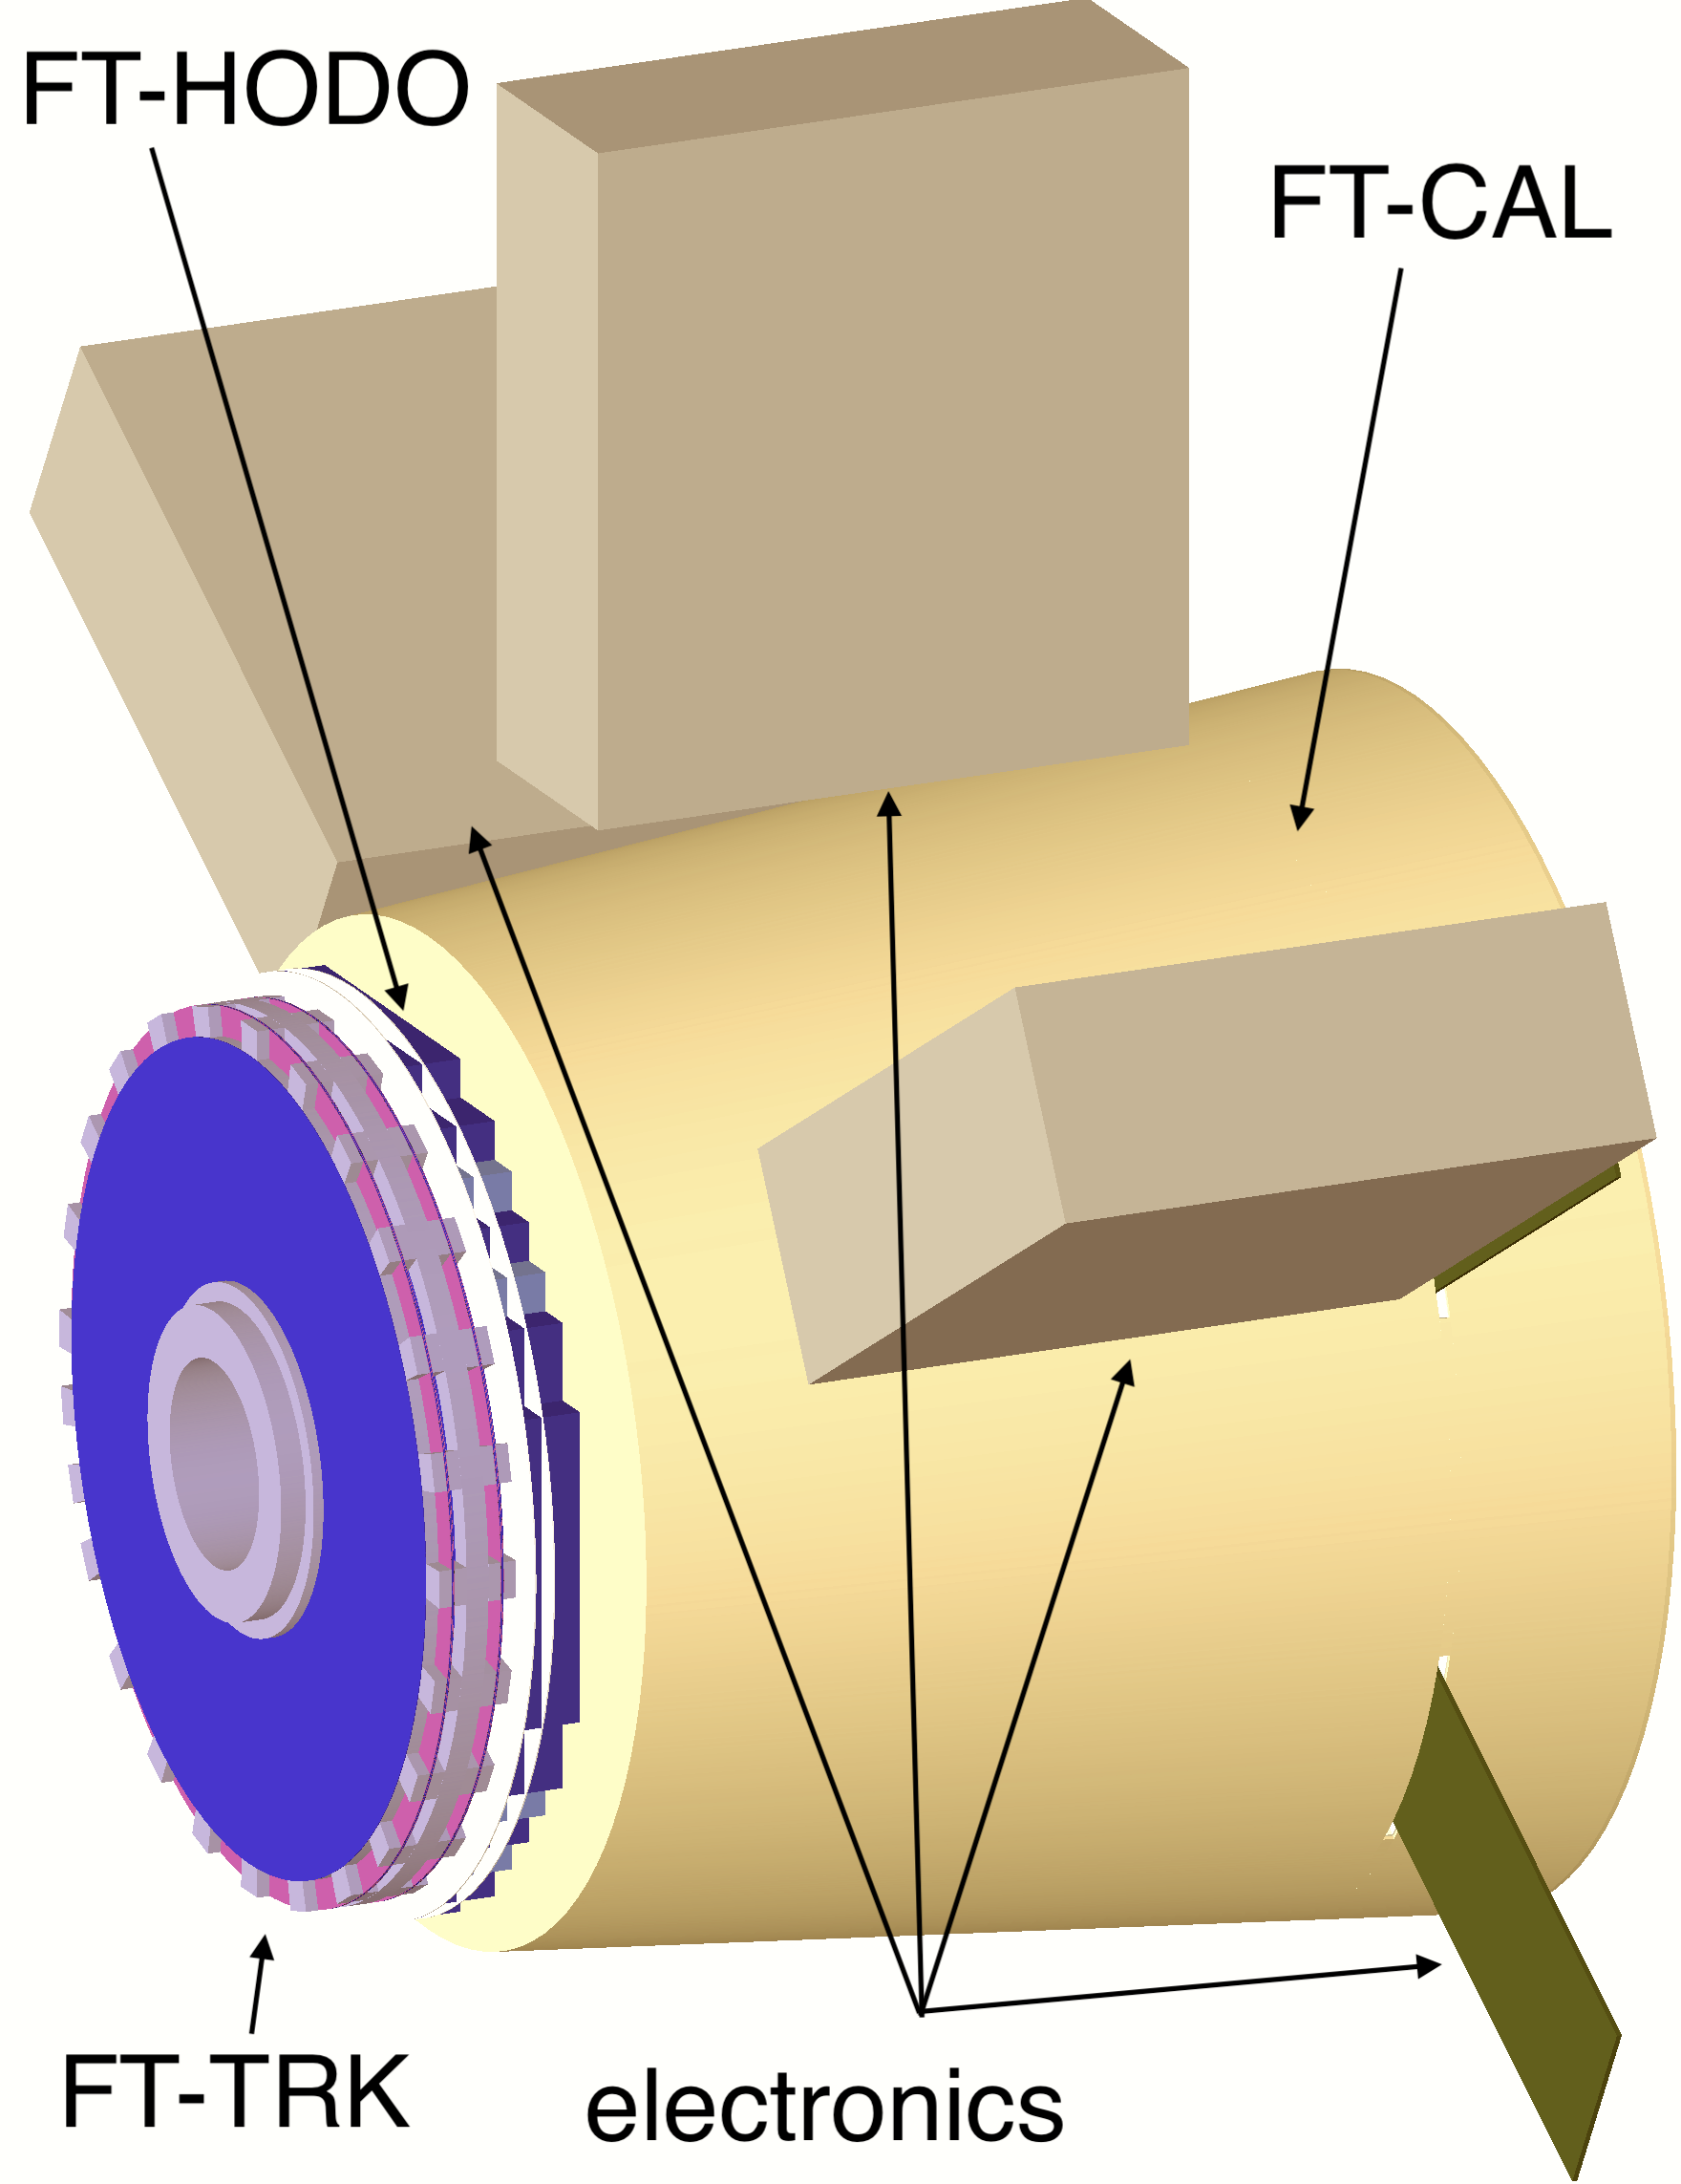
\includegraphics[width=0.99\columnwidth,keepaspectratio]{img/ftGeometry.png}
	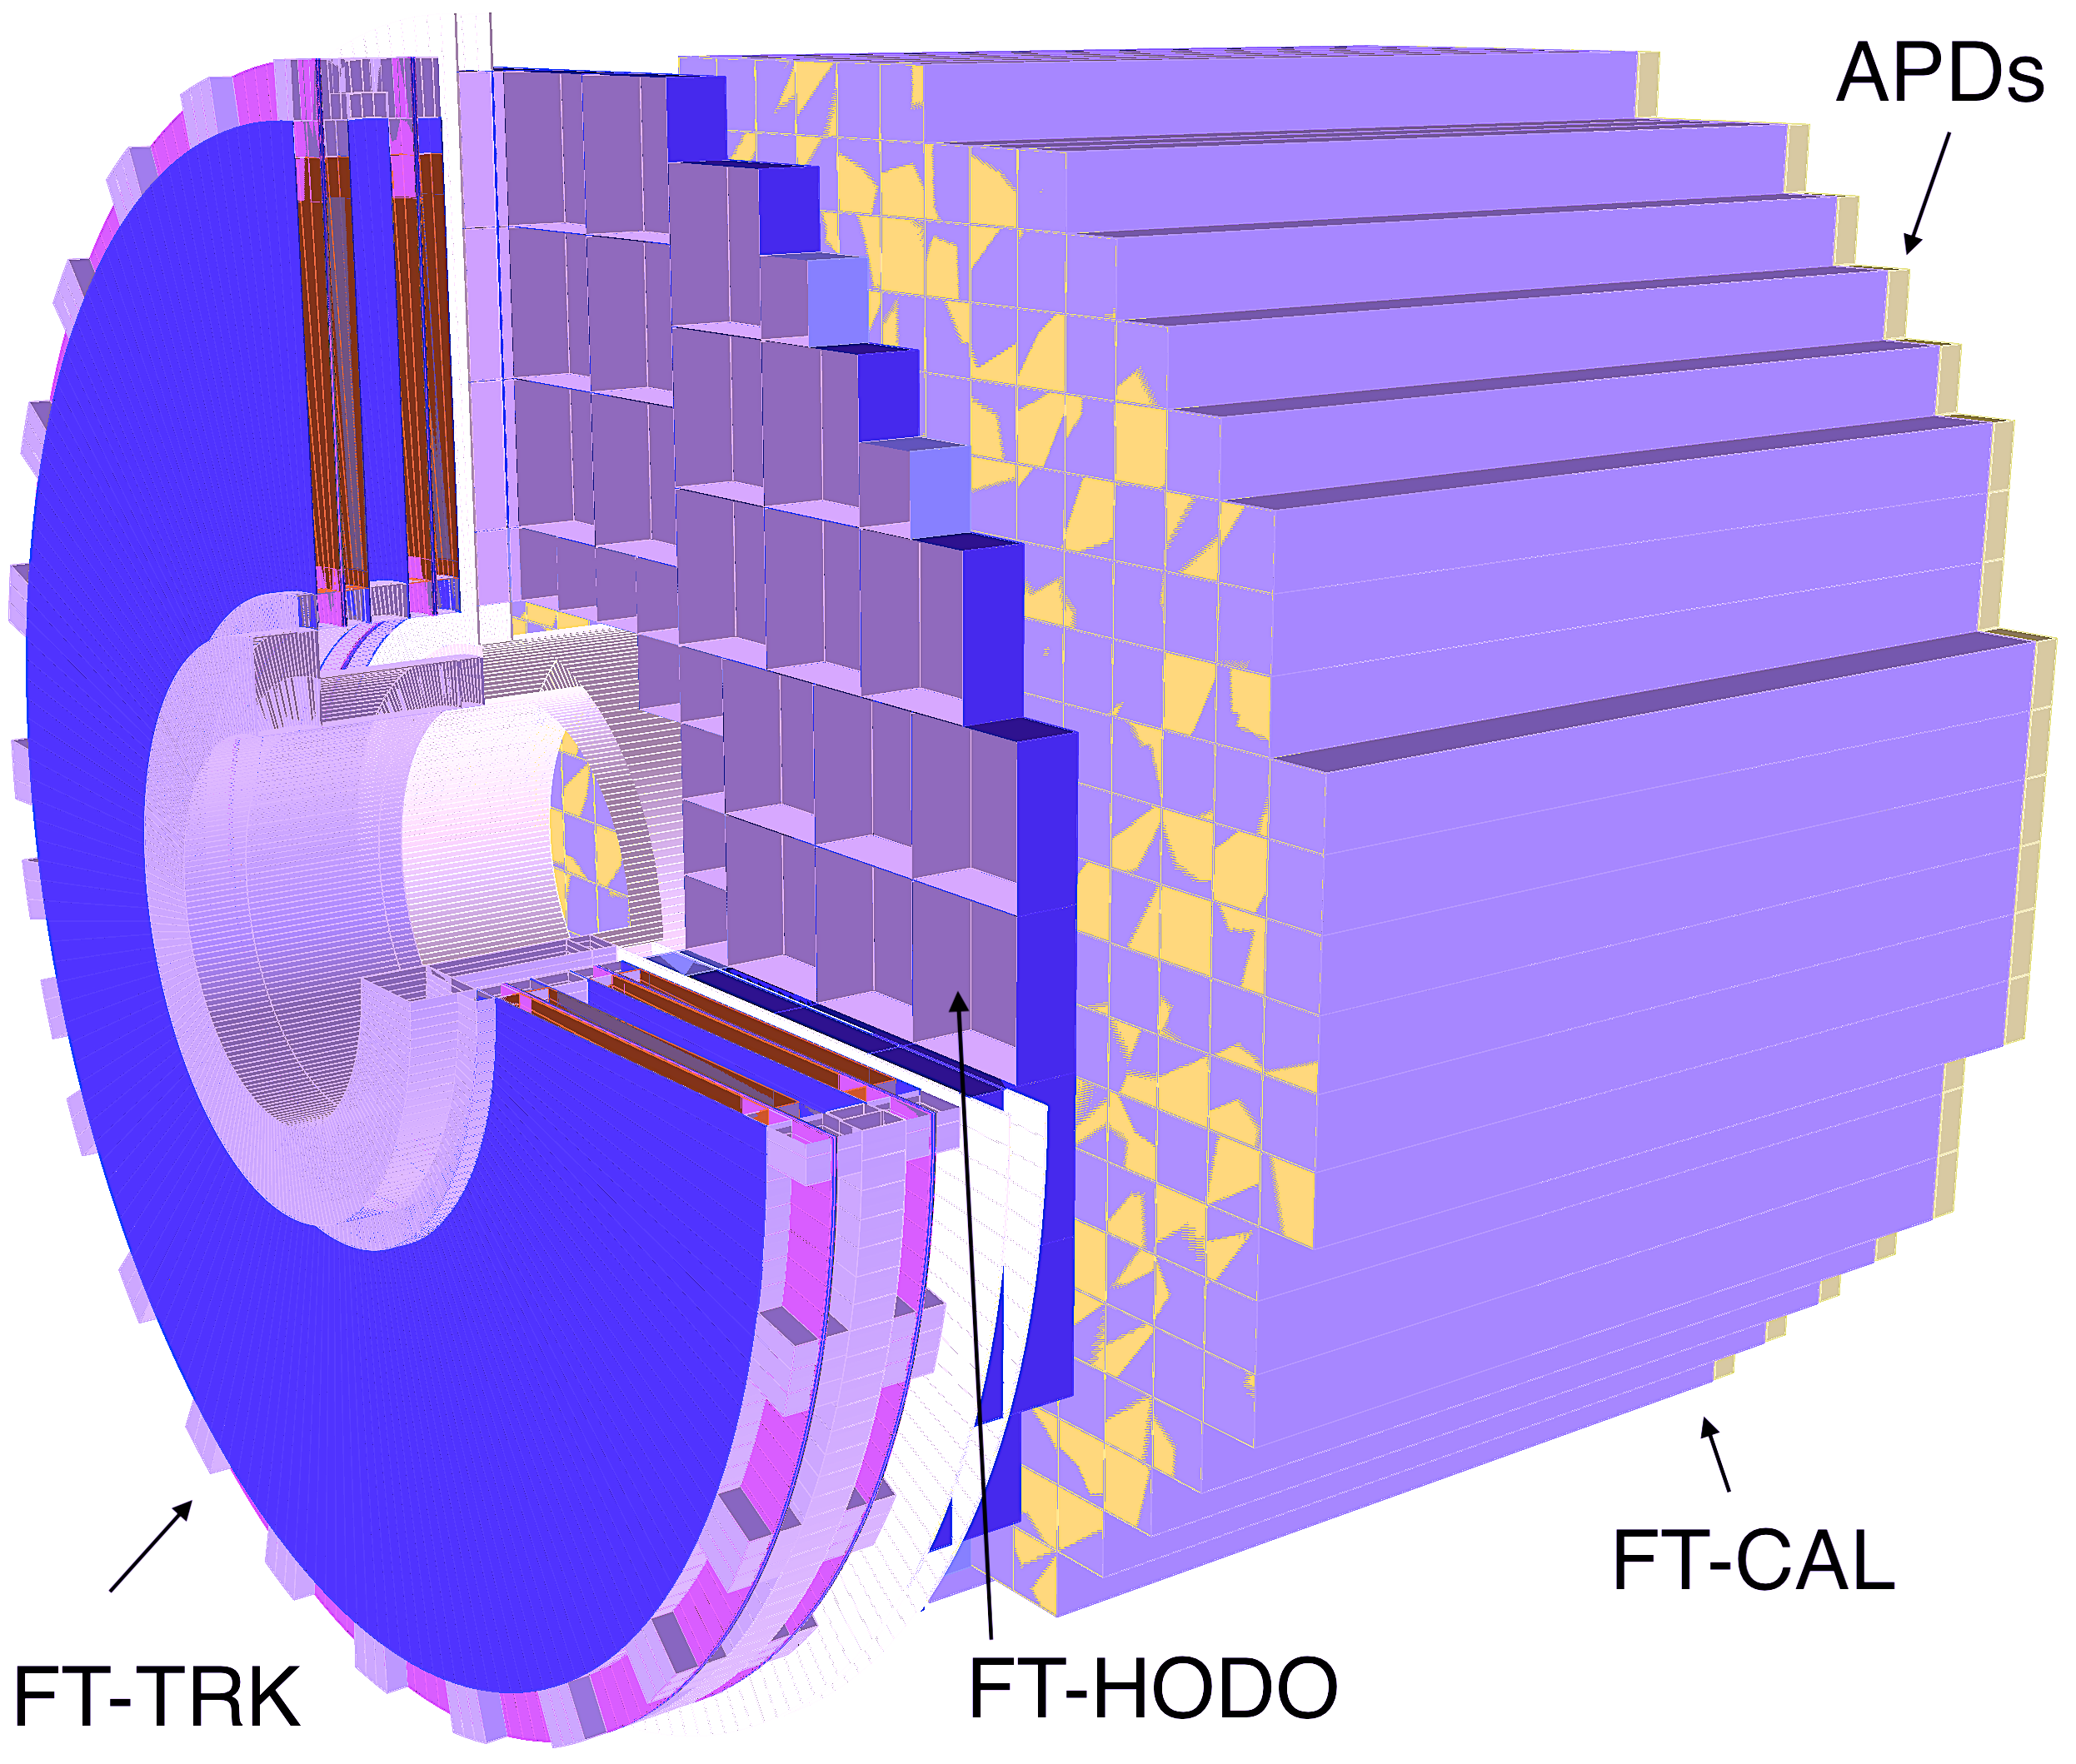
\includegraphics[width=0.99\columnwidth,keepaspectratio]{img/ftDetails.png}
	\caption{Top: the FT detector implementation in GEMC. The boxes surrounding FT-CAL contain the electronics.
			 Bottom: details of the the three subsystems implementation. As seen by the beam (impinging from the left):
             the disks form the FT-TRK; the FT-HODO scintillators just behind the tracker;
			 and the FT-CAL crystals. }
	\label{fig:ftGeometry}
\end{figure}

The FT-TRK digitization provides the ADC value calculated using the total energy deposited (after hit sharing).
There is no timing information in the FT-TRK output.

For FT-CAL hits, the energy deposited is converted first to the charge produced at the end of the electronics chain composed
by an avalanche photodiode (APD) and pre-amplifier, and then to an ADC.
The first conversion is based on the measured charge for cosmic rays that deposit a known energy in the crystals,
while the second conversion is based on the FADC conversion factor. A smearing on the final ADC values is added,
accounting for the Poisson distribution of photo-electrons produced by the photosensor, the Gaussian noise of the
photosensor, and of the preamplifier. All parameters, the number of photo-electrons per MeV of energy deposited,
the RMS width of the APD noise, and of the preamplifier input noise, have been tuned to the experimental data.

The same approach is adopted to process FT-HODO hits, in which the deposited energy is first converted to charge and then to ADC.
The smearing in this case accounts only for the Poisson distribution of the measured number of photo-electrons,
which dominates over other sources because of the relatively small number of photo-electrons per MeV of energy deposition.

The TDC of FT-CAL hits is computed from the time of the energy deposition, accounting for the speed of the scintillation light in
the crystal and the distance to the photosensor, assuming a known time-to-TDC conversion factor. A Gaussian smearing on the
resulting TDC is added based on a fixed RMS resolution derived from the experimental measurements.

Similarly, the TDC of FT-HODO hits is derived from the time of a given energy deposition, adding a fixed offset before the
conversion from time to TDC and a Gaussian smearing. As in previous cases, all relevant parameters have been tuned to the
observed detector response.
The digitized output bank variables are summarized in Table \ref{tab:ftBank}

\begin{table}[h]
	\begin{center}
		\begin{tabular}{| c | c | c |}
			\hline \hline
			Variable            & Description      \\
			\hline
		                         & Tracker         \\
			\hline
                         sector  &     sector      \\
                          layer  &      layer      \\
                      component  &  component      \\
                            ADC  &        ADC      \\
			\hline
		                         & Hodoscope       \\
			\hline
						 sector  &     sector      \\
                          layer  &      layer      \\
                      component  &  component      \\
                            ADC  &        ADC      \\
                            TDC  &        TDC      \\
			\hline
								 & Calorimeter     \\
			\hline
				         sector  &     sector      \\
				   	      layer  &      layer      \\
					  component  &  component      \\
							ADC  &        ADC      \\
							TDC  &        TDC      \\
			\hline \hline
		\end{tabular}
	\end{center}
	\caption{The digitized FT banks for the tracker, hodoscope, and calorimeter}\label{tab:ftBank}
\end{table}

\noindent The time window  of the Tracker is set to to 132 ns: all Geant4 steps within the same strip and time window are collected in one hit.
The time window of the hodoscope and calorimeters are set to 400 ns: all Geant4 steps within the same paddles and time window
will be collected on one hit in each system.

\section{Drift Chambers (DC)}


\subsection{Geometry}

\subsubsection{Geometry Git Location}

\subsection{Process ID}

\subsection{Digitization}



\subsubsection{ADC}
\subsubsection{TDC}

\subsubsection{Summary of CCDB Table used}

\subsection{Digitized Bank}

\subsubsection{Time Window}

\subsubsection{Process Routine Git Repository Location}


The DC hit process routine location in git is \url{https://github.com/gemc/source/blob/master/hitprocess/clas12/dc_hitprocess.cc}

\subsection{Low Threshold Cherenkov Counter (LTCC)}

\subsubsection{Geometry}
The LTCC mirror geometry is implemented through the native GEMC geometry API. The elliptical mirrors are made through a subtraction of
two ellipsoids. The hyperbolic mirrors are built using Geant4 ``polycones'' approximating the mathematical shape using about 30 segments.
The cylindrical mirrors are made from cuts of cylinder volumes.

The LTCC Winston cones (WC) are of three types: small, medium, and large. Three CAD models are tessellated and imported in the simulation, and
then copied into 36 WC / sector using the perl API.

Finally, the LTCC box, mirror support structure, and additional support hardware are imported directly from the engineering CAD models.
\F{ltccGeometry} shows details of the geometry implementation.

\begin{figure}
	\centering
	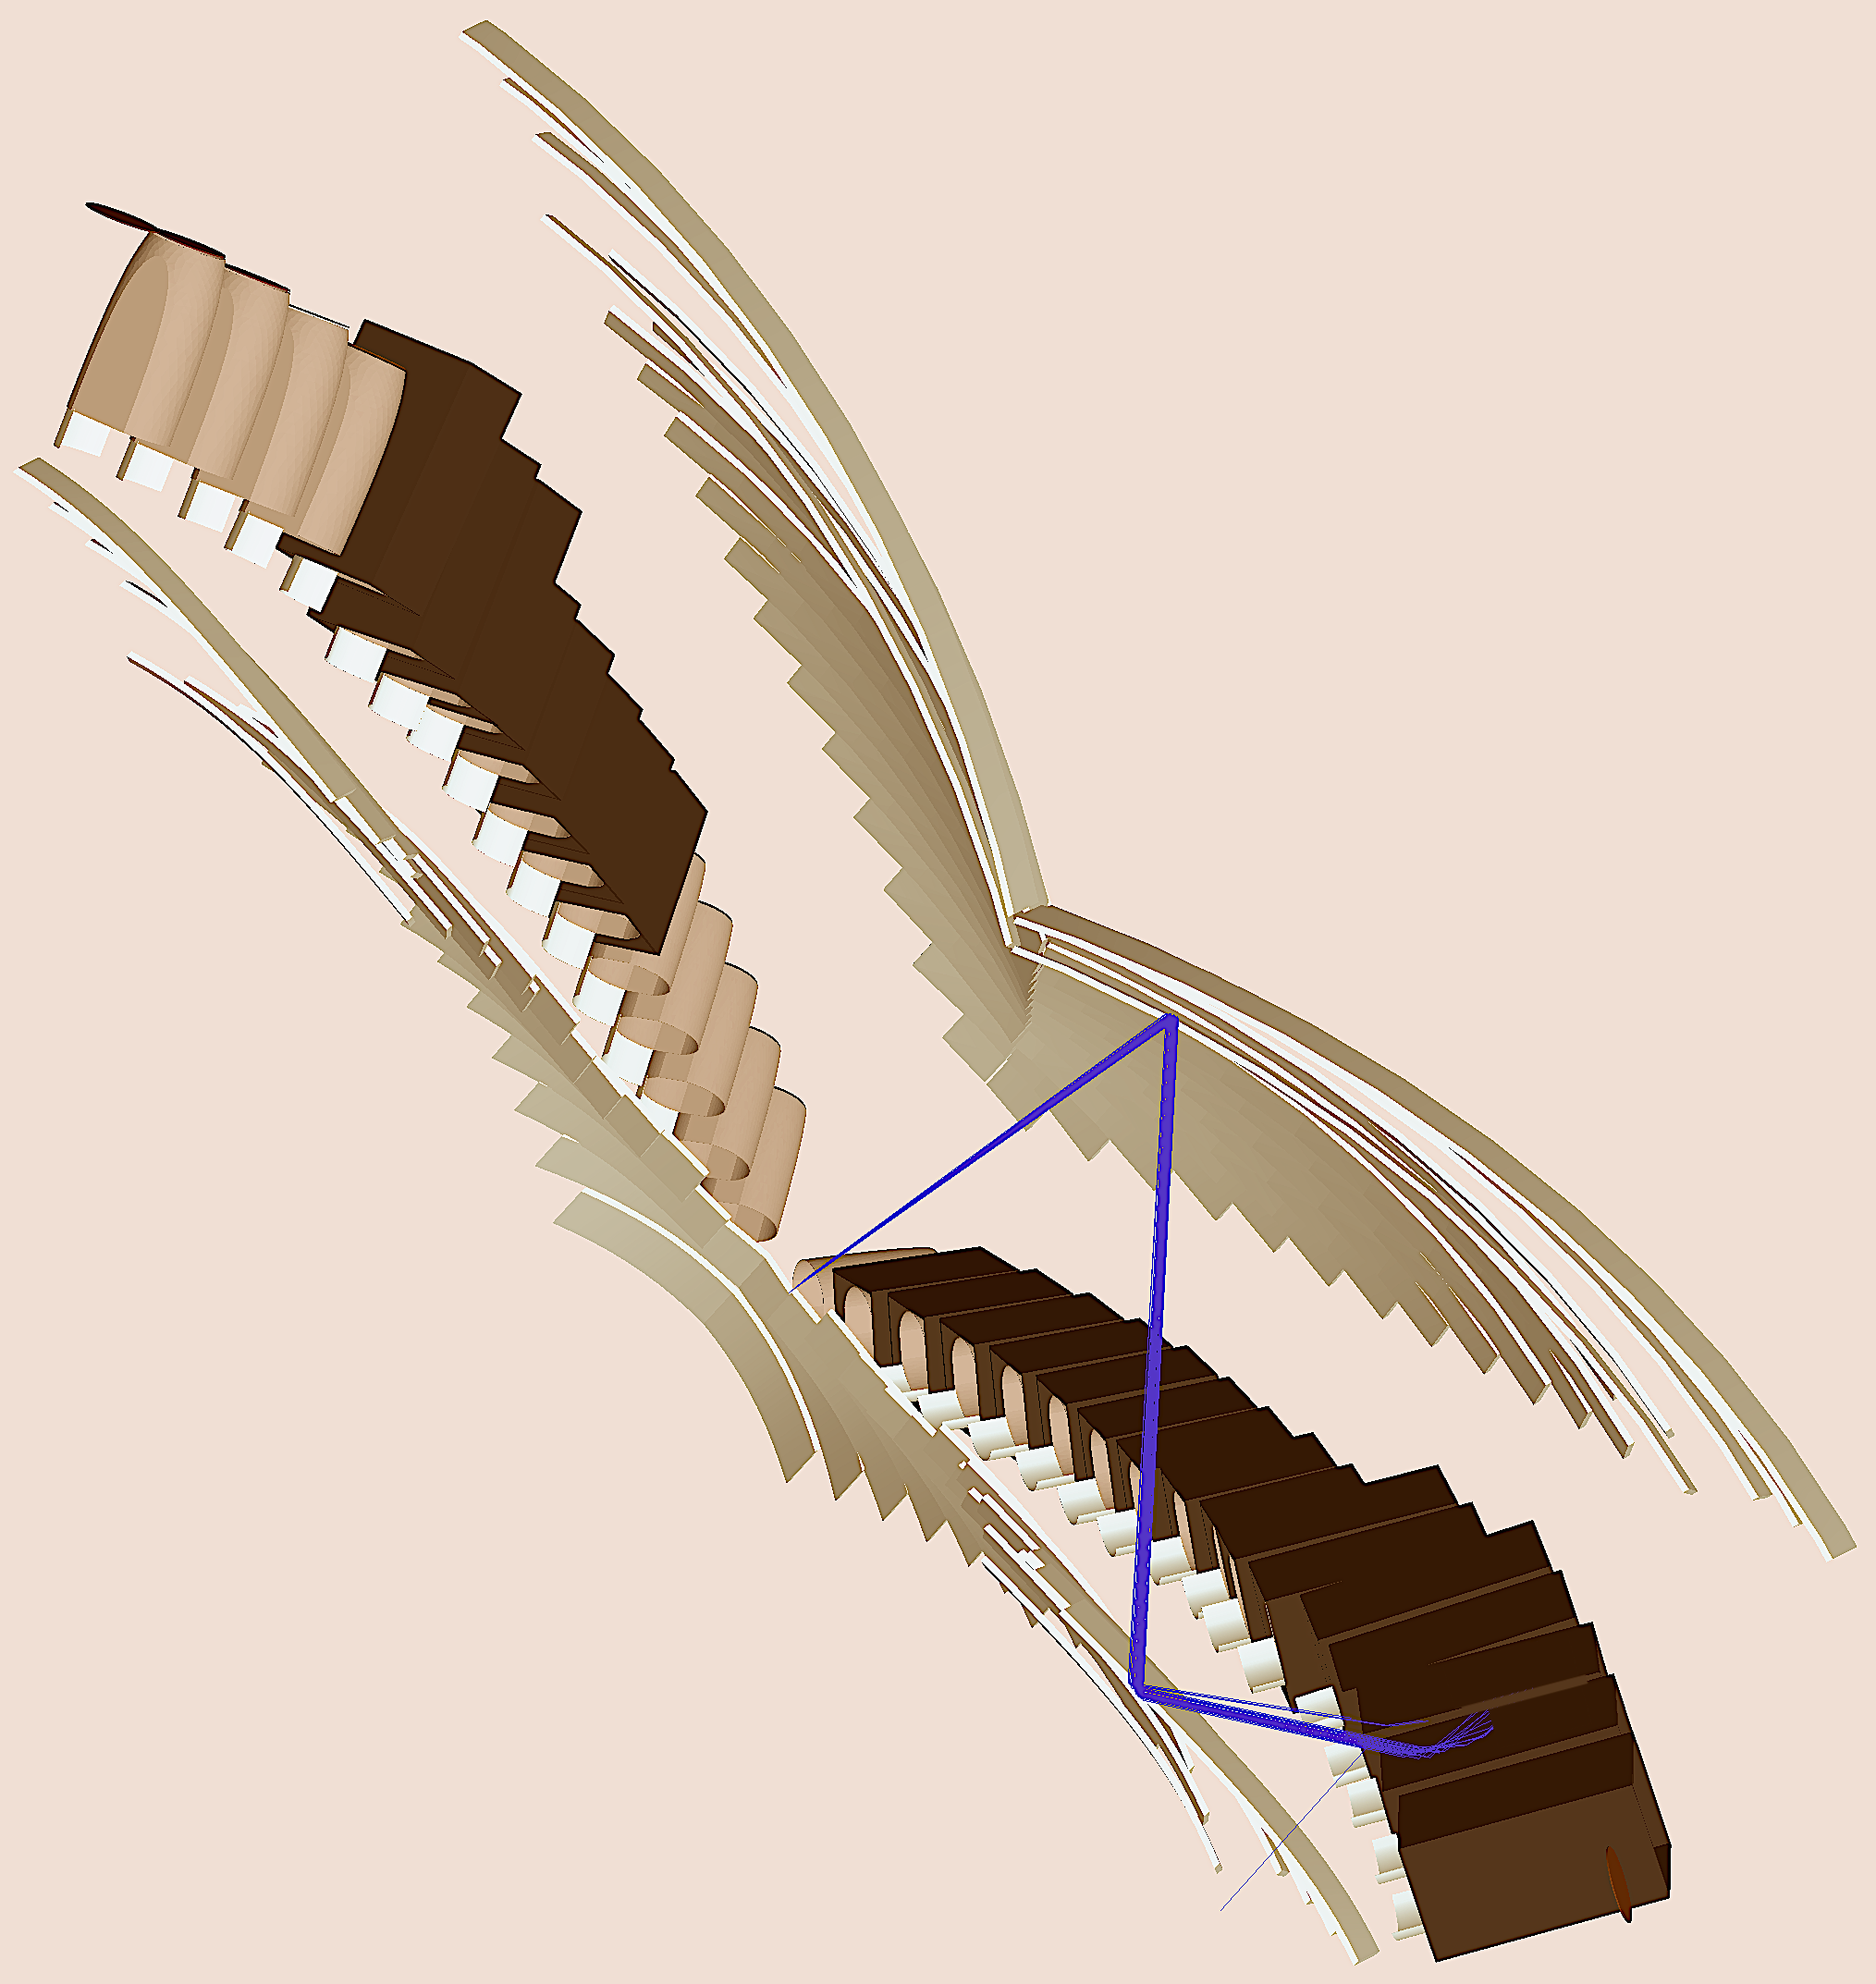
\includegraphics[width=0.99\columnwidth, keepaspectratio]{img/ltccGeometry.png}
	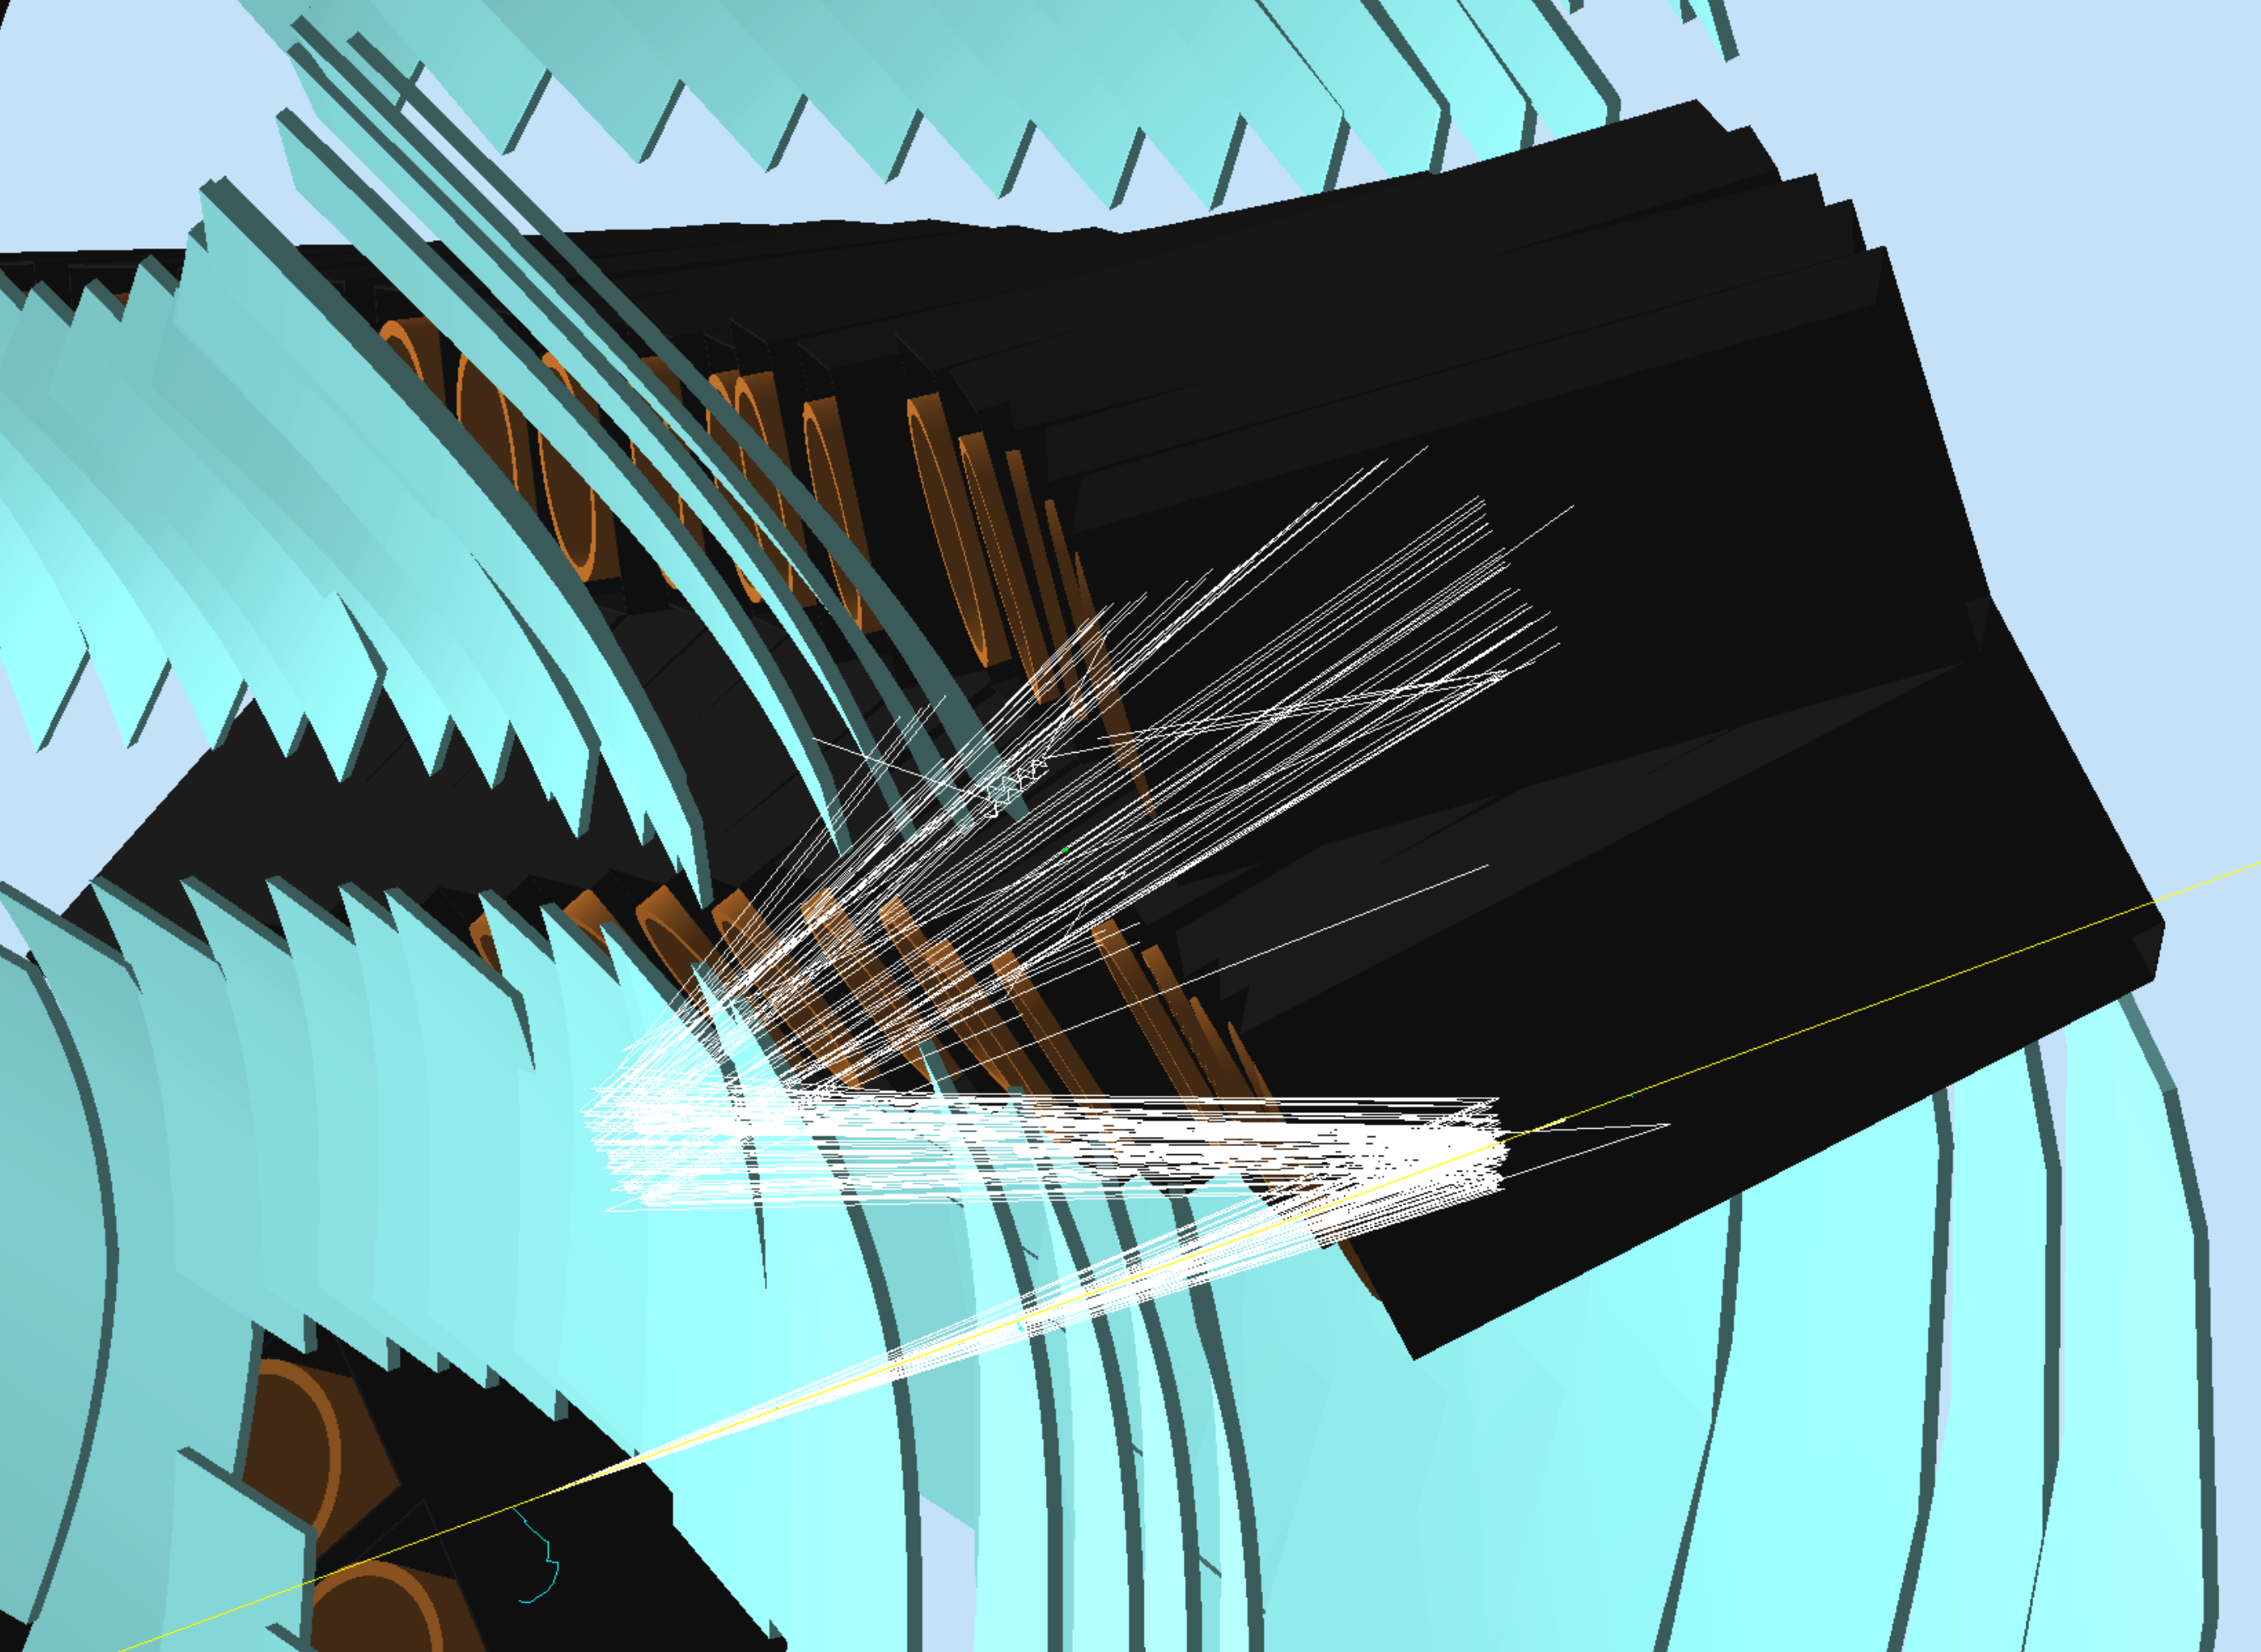
\includegraphics[width=0.99\columnwidth, keepaspectratio]{img/ltccDetail.png}
	\caption{Top: a 6 GeV pion passing through the LTCC gas volume and emitting Cherenkov photons. The light cone
            bounces from the elliptical to the hyperbolic mirrors to the Winston cone, and finally reaches the PMT.
            Bottom: details of the hardware inside the LTCC simulation system: the box frame and the WC are
            imported from CAD. The mirrors, shields, and PMTs are made with Geant4 volumes. One of the PMT shields
            in this picture was removed to show the WC. The PMT is simulated as a disk attached to the WC. }
	\label{fig:ltccGeometry}
\end{figure}

The refractive index of the $C_4F_{10}$ radiator gas and its transparency is included in the material optical properties and taken
into account during the Geant4 transportation of the photons.
Similarly for the reflectivity of the mirrors and Winston cones.
The quantum efficiency associated with the PMT photo-cathodes is taken into account in
the digitization routine.

\subsubsection{Digitization}

Photons that impinge on the PMT faces are processed with the digitization routine.
Each photon collected is input to the quantum efficiency algorithm at its wavelength to decide if it is detected.
The ADC energy is calculated and smeared using the single photo-electron peak position and width from the calibration database.
The time average of all the photons is saved in the output.
The digitized output bank variables are summarized in Table \ref{tab:ltccBank}.

\begin{table}[h]
	\begin{center}
		\begin{tabular}{| c | c | c |}
			\hline \hline
			Variable & Description                                         \\
			\hline
             sector  &                                     CLAS12 sector   \\
               side  &                               left or right index   \\
            segment  &                                           segment   \\
                ADC  &                                               ADC   \\
               time  &                           average time of the hit   \\
               nphe  &                  number of photo-electrons arrived   \\
              npheD  &                 number of photo-electrons detected   \\
               hitn  &                                        hit number   \\
			\hline \hline
		\end{tabular}
	\end{center}
	\caption{The digitized LTCC bank.}\label{tab:ltccBank}
\end{table}

The time window  of the LTCC is set to 5 ns: all Geant4 steps within the same PMT and time window are collected in one hit.

\subsection{Ring-Imaging Cherenkov (RICH)}

One of the six CLAS12 Forward Carriage sectors has been equipped with a Ring Imaging Cherenkov detector \cite{rich-nim}.

\subsubsection{Geometry}
The RICH mirror geometry is implemented through both of the native GEMC geometry API and imports from the engineering model STEP files.
The spherical mirrors are made through Geant4 boolean intersections of spheres and planes.
Since the array of 391 PMTs is inside the CLAS12 acceptance, particular care went into implementing in the
simulation the details of the PMT hardware and materials: the PMTs are Geant4 aluminum boxes containing the electronics components
(including the adapter, ASIC and FPGA boards), the window, the photocathodes.
Each PMTs contain 64 pixel. The identification of the pixel is done in the process identification routine.
The aerogel are Geant4 boxes.
The RICH box, mirror support structure, and additional support hardware are imported directly from the engineering CAD models.
\F{richGeometry} shows details of the geometry implementation.

\begin{figure}
	\centering
	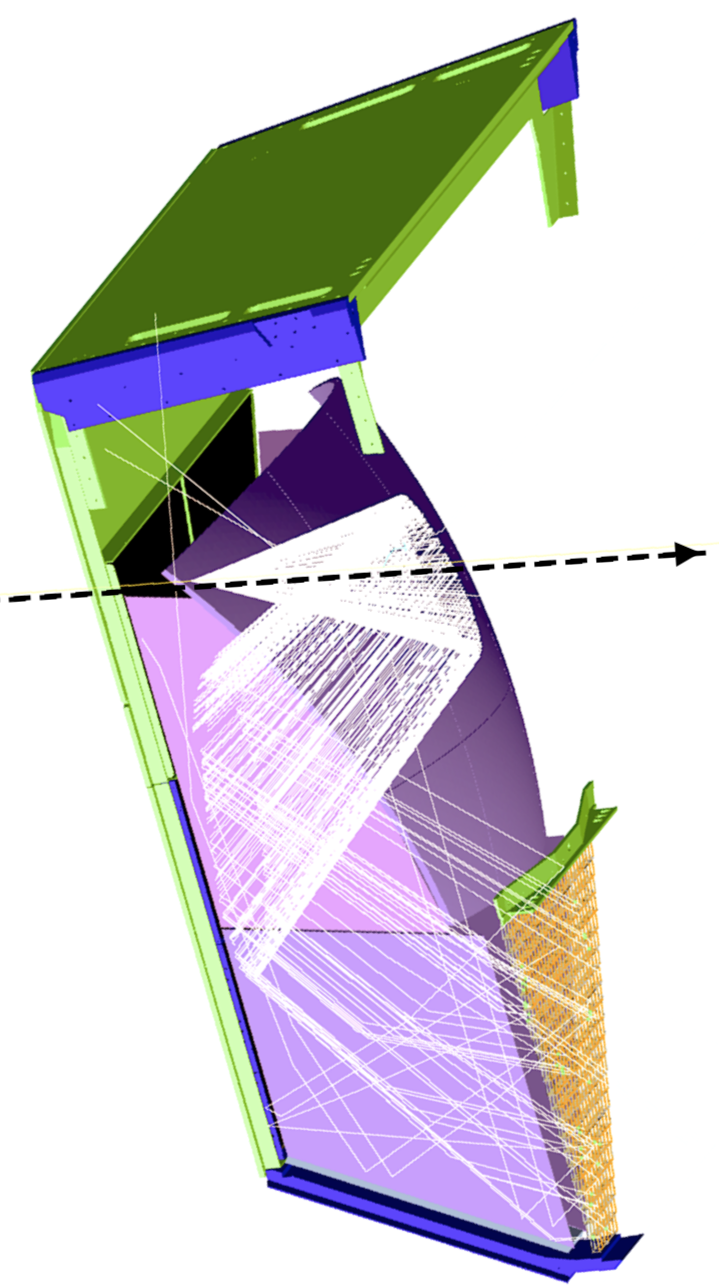
\includegraphics[width=0.99\columnwidth, keepaspectratio]{img/richGeometry.png}
	\caption{The implementation of the RICH geometry. Beam is incident from the left. A 4 GeV kaon produces a Cherenkov light cone.
			 Part of the cone reflects onto the spherical mirror and into the PMT array. The remaining photons go through the aerogel tiles
			 and bounce off the planar mirror onto the PMT array. All inefficiencies are taken into account by using the aerogel refractive index
			 and its transparency. }
	\label{fig:richGeometry}
\end{figure}

The refractive index of the aerogel and its transparency is included in the material optical properties and taken
into account during the Geant4 transportation of the photons.
Similarly for the reflectivity of the mirrors. The quantum efficiency associated with the PMT photocathodes is taken into account in the digitization routine.

\subsubsection{Process ID}
At each Geant4 step, the local coordinates in the PMT volume are used to calculate the pixel number within that PMT.

\subsubsection{Digitization}

Photons that impinge on the PMT faces are processed with the digitization routine.
Each photon collected is input to the quantum efficiency algorithm at its wavelength to decide if it is detected.
The ADC energy is calculated and smeared using the single photo-electron peak position and width from the calibration database.
The time average of all the photons is saved in the output.
The digitized output bank variables are summarized in Table \ref{tab:richBank}.

\begin{table}[h]
	\begin{center}
		\begin{tabular}{| c | c | c |}
			\hline \hline
			Variable & Description                                         \\
			\hline
             sector  &                                     CLAS12 sector   \\
                pmt  &                                        PMT number   \\
              pixel  &                       pixel number within the PMT   \\
                ADC  &                                               ADC   \\
               time  &                           average time of the hit   \\
               nphe  &                  number of photoelectrons arrived   \\
              npheD  &                 number of photoelectrons detected   \\
               hitn  &                                        hit number   \\
			\hline \hline
		\end{tabular}
	\end{center}
	\caption{The digitized RICH bank.}\label{tab:richBank}
\end{table}

The time window  of the RICH is set to 5 ns: all Geant4 steps within the same PMT pixel and time window are collected in one hit.


\section{Forward Time-Of-Flight (FTOF)}


\subsection{Geometry}

The FTOF geometry is implemented through the COATJAVA geometry service.
The service provides the geant4 definitions that are read by the GEMC perl api to build the geometry database.

All scintillators are geant4 volumes.
Each scintillator is a G4Box embedded in a G4Trapezoid mother volume made of air, see \F{ftofGeometry}.

\begin{figure}
	\centering
	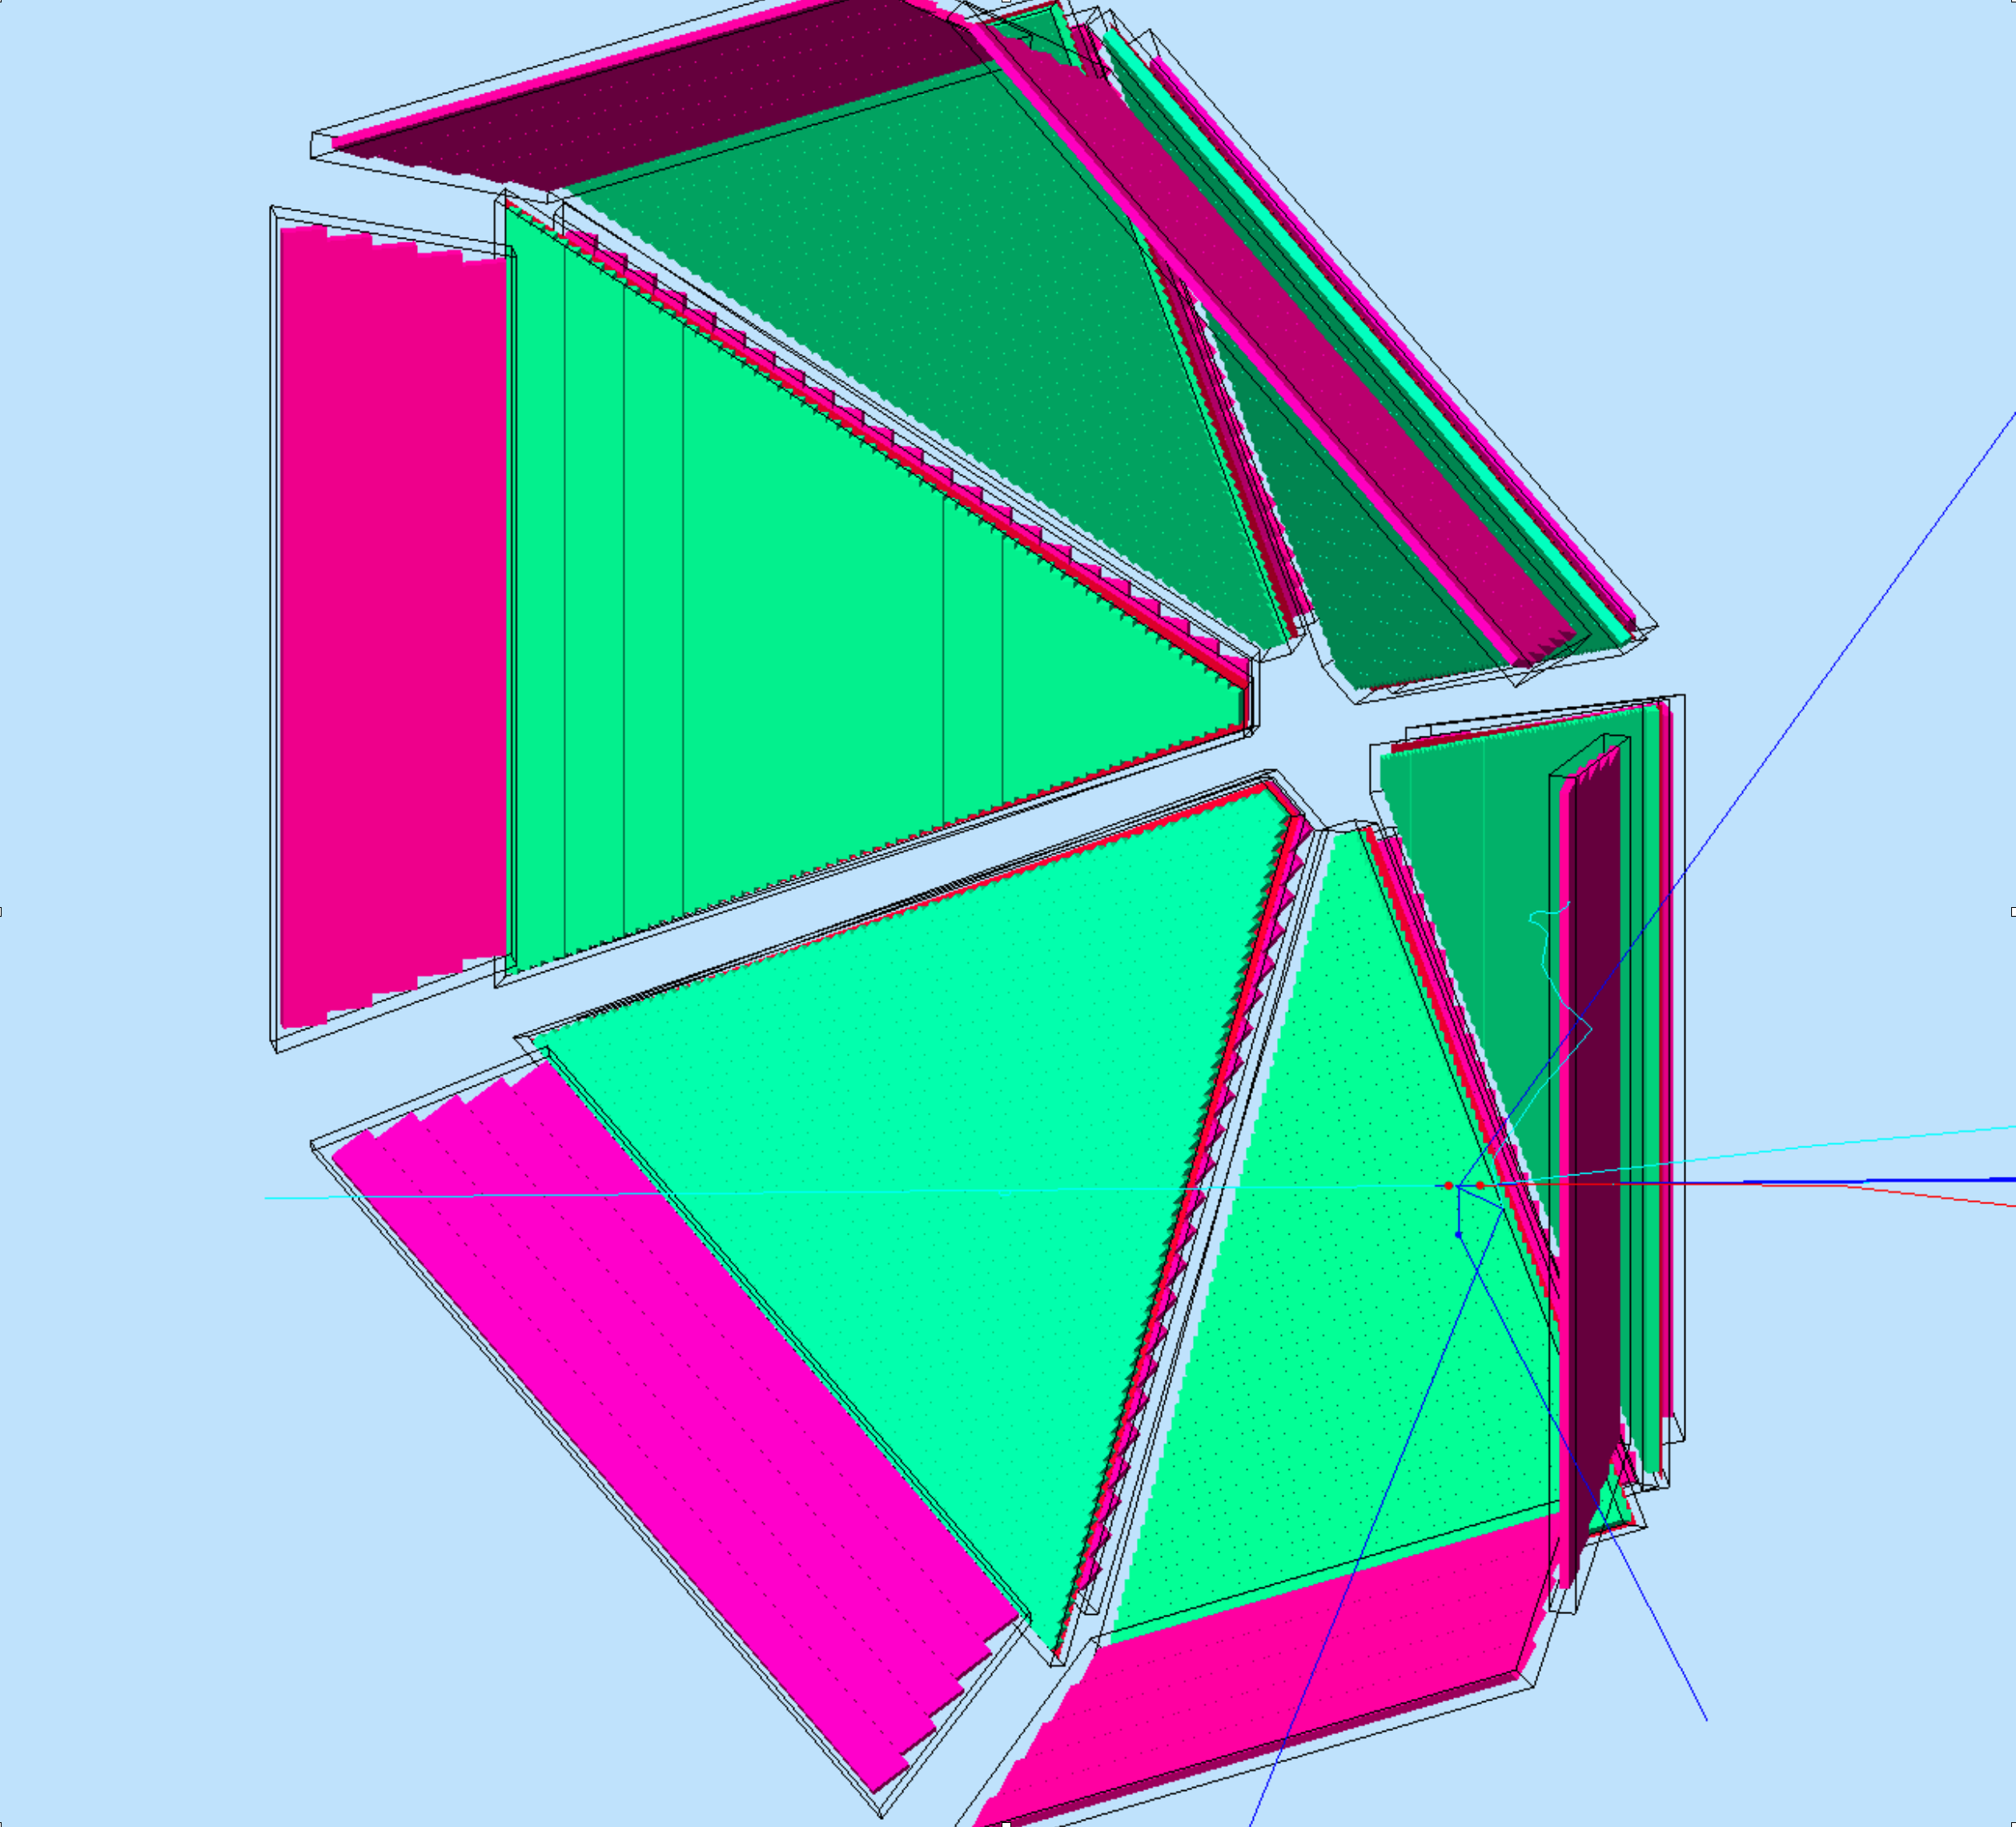
\includegraphics[width=0.95\columnwidth,keepaspectratio]{img/ftofGeometry.png}
	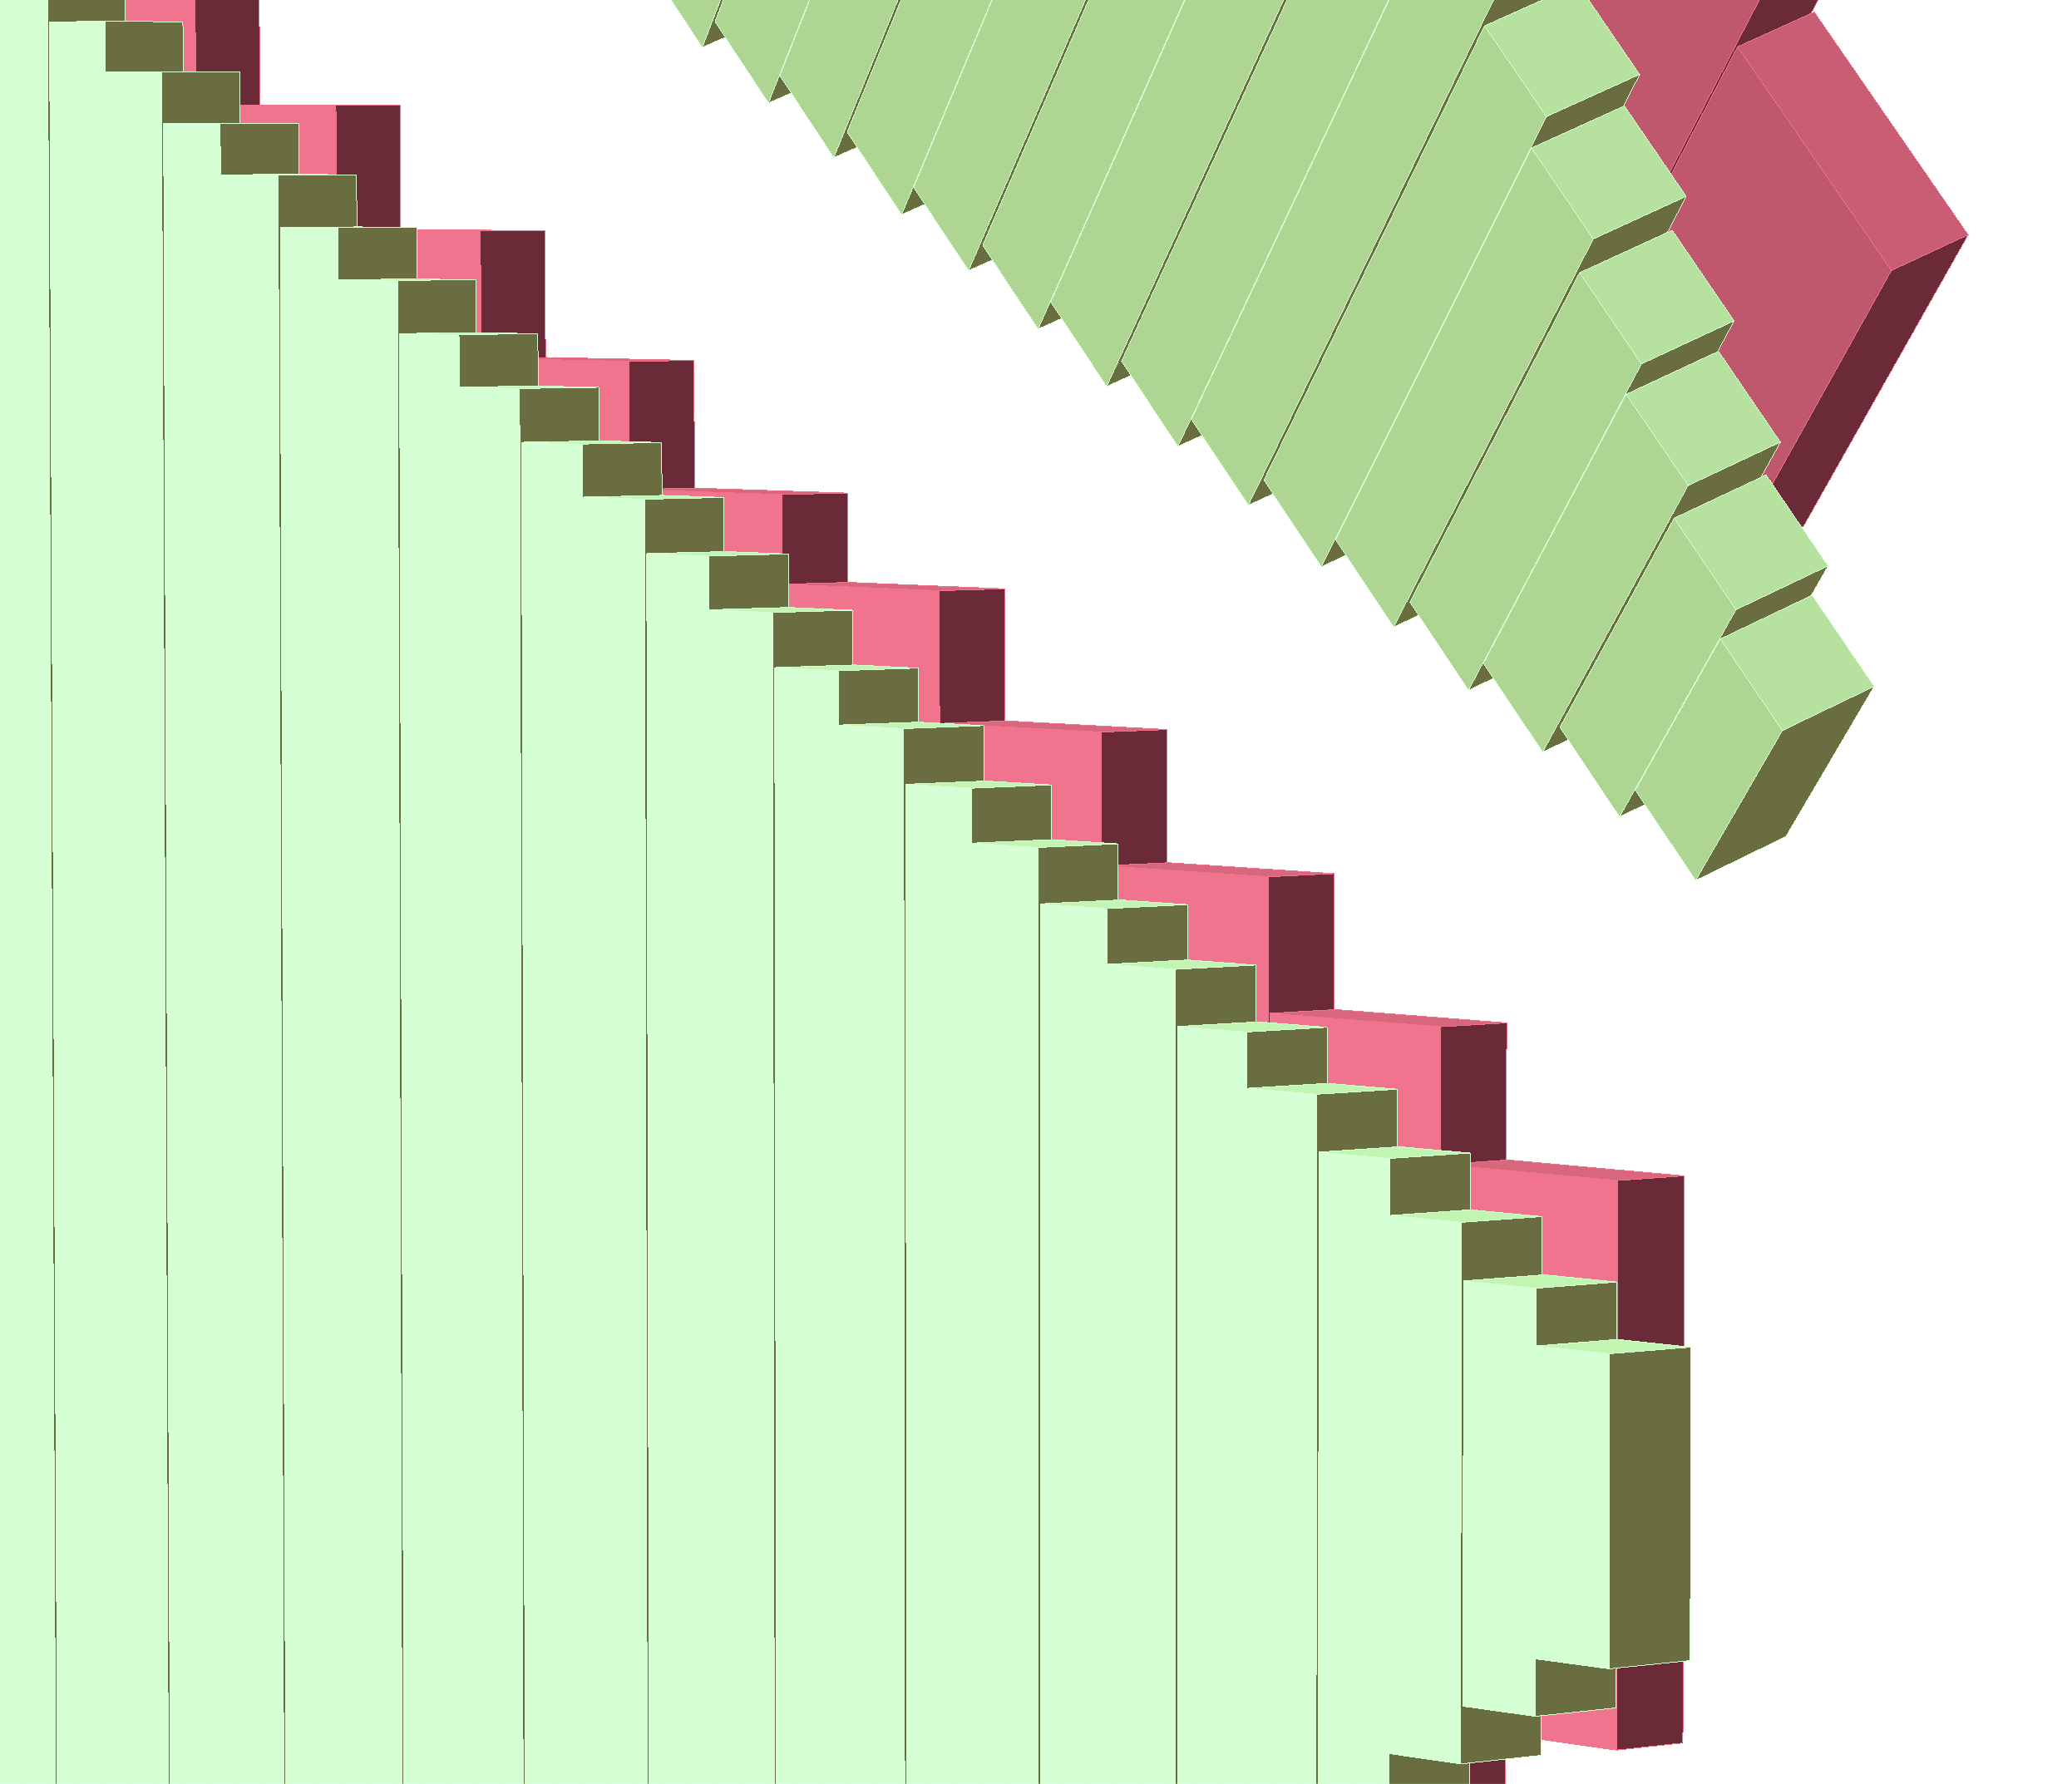
\includegraphics[width=0.95\columnwidth,keepaspectratio]{img/ftofDetail.png}
	\caption{Top: the GEMC implementation of the FTOF geometry. The paddles are G4Boxes, embedded in trapezoid representing the mother volumes of each panel.
            Bottom: a zoom-in of the implementation shows the details of the individual paddles for Panel 1B (green) and Panel 1A (purple) }
	\label{fig:ftofGeometry}
\end{figure}

\subsubsection{Geometry Git Location}
The github location of the gemc perl api script is \url{https://github.com/gemc/detectors/tree/master/clas12/ftof}.

The geometry service definitions in coatjava is \url{https://github.com/JeffersonLab/clas12-offline-software/blob/development/common-tools/clas-jcsg/src/main/java/org/jlab/detector/geant4/v2/FTOFGeant4Factory.java}

\subsection{Process ID}

Each hit in the paddles is produces in two identical hits with the identifier variable "side" sets to 0 (for the left side PMT) and 1 (for right side PMT).
The hits are then processed independently through the ftof hit process routine.

\subsection{Digitization}

\subsubsection{ADC}
The energy deposited is reduced based on the position on the paddle using the calibration attenuation length. It is then corrected by a gain factor
to account for the fact that the HV are adjusted so that the geometeric mean sqrt(L*R) is independent of counter length.

The corrected energy is converted to the theoretical number of photos $N_{th}$ using the constant $500 \gamma / MeV $. A poissonian is used to
calculate the actual number of photons $N_{actual}$ and the resulting ``smeared`` energy is the converted to adc using the FADC conversion factor.

\subsubsection{TDC}

The absolute hit time is corrected by:

\begin{itemize}
	\item the effective velocity (from CCDB)
	\item the time walk correction, calculated from the smeared energy
	\item a panel to panel factor (from CCDB)
	\item a left/rigth time offset factor (from CCDB)
	\item an RF correction (from CCDB)
\end{itemize}

The time is then smeared by a $\sigma$ resolution read from CCDB using a gaussian function and then digitized using a TDC conversion factor.

\subsubsection{Summary of CCDB Table used}
\begin{itemize}
	\item /calibration/ftof/attenuation
	\item /calibration/ftof/effective\_velocity
	\item /calibration/ftof/status
	\item /calibration/ftof/gain\_balance
	\item /calibration/ftof/time\_walk
	\item /calibration/ftof/time\_offsets
	\item /calibration/ftof/tdc\_conv
	\item /daq/tt/ftof
\end{itemize}

\subsection{Digitized Bank}
The digitized output bank has $ID=1000$, and the variables are summarized in Table \ref{tab:ftofBank}

\begin{table}[h]
	\begin{center}
		\begin{tabular}{| c | c | c |}
			\hline \hline
			Variable         & Description  & Tag  \\
			\hline
              sector  &                             sector number  &    1 \\
               layer  &               layer (1: 1A, 2: 1B, 3: 2B)  &    2 \\
              paddle  &                             paddle number  &    3 \\
                side  &                PMT side (0 Left, 1 Right)  &    4 \\
                 ADC  &                                       ADC  &    5 \\
                 TDC  &                                       TDC  &    6 \\
                ADCu  &                             ADC unsmeared  &    7 \\
                TDCu  &                             TDC unsmeared  &    8 \\
                hitn  &                                hit number  &   99 \\
			\hline \hline
		\end{tabular}
	\end{center}
	\caption{Summary of LTCC Electronics}\label{tab:ltccChannels}
\end{table}


\subsubsection{Time Window}

The timewindow of the

\subsubsection{Process Routine Git Repository Location}
The FTOF hit process routine location in git is \url{https://github.com/gemc/source/blob/master/hitprocess/clas12/ftof_hitprocess.cc}



\section{Electromagnetic Calorimeter (EC) and pre-shower calorimeter (PCAL)}

\subsection{Geometry}

\subsubsection{Geometry Git Location}

\subsection{Process ID}

\subsection{Digitization}

\subsubsection{Summary of CCDB Table used}

\subsection{Digitized Bank}

\subsubsection{Time Window}

\subsubsection{Process Routine Git Repository Location}



\subsection{Solenoid and Torus Magnets}


\subsubsection{Geometry}
The solenoid geometry is produced with the GEMC perl API. The solenoid is a single polycone volume, shown in \F{solenoid}.
\begin{figure}[h]
	\centering
	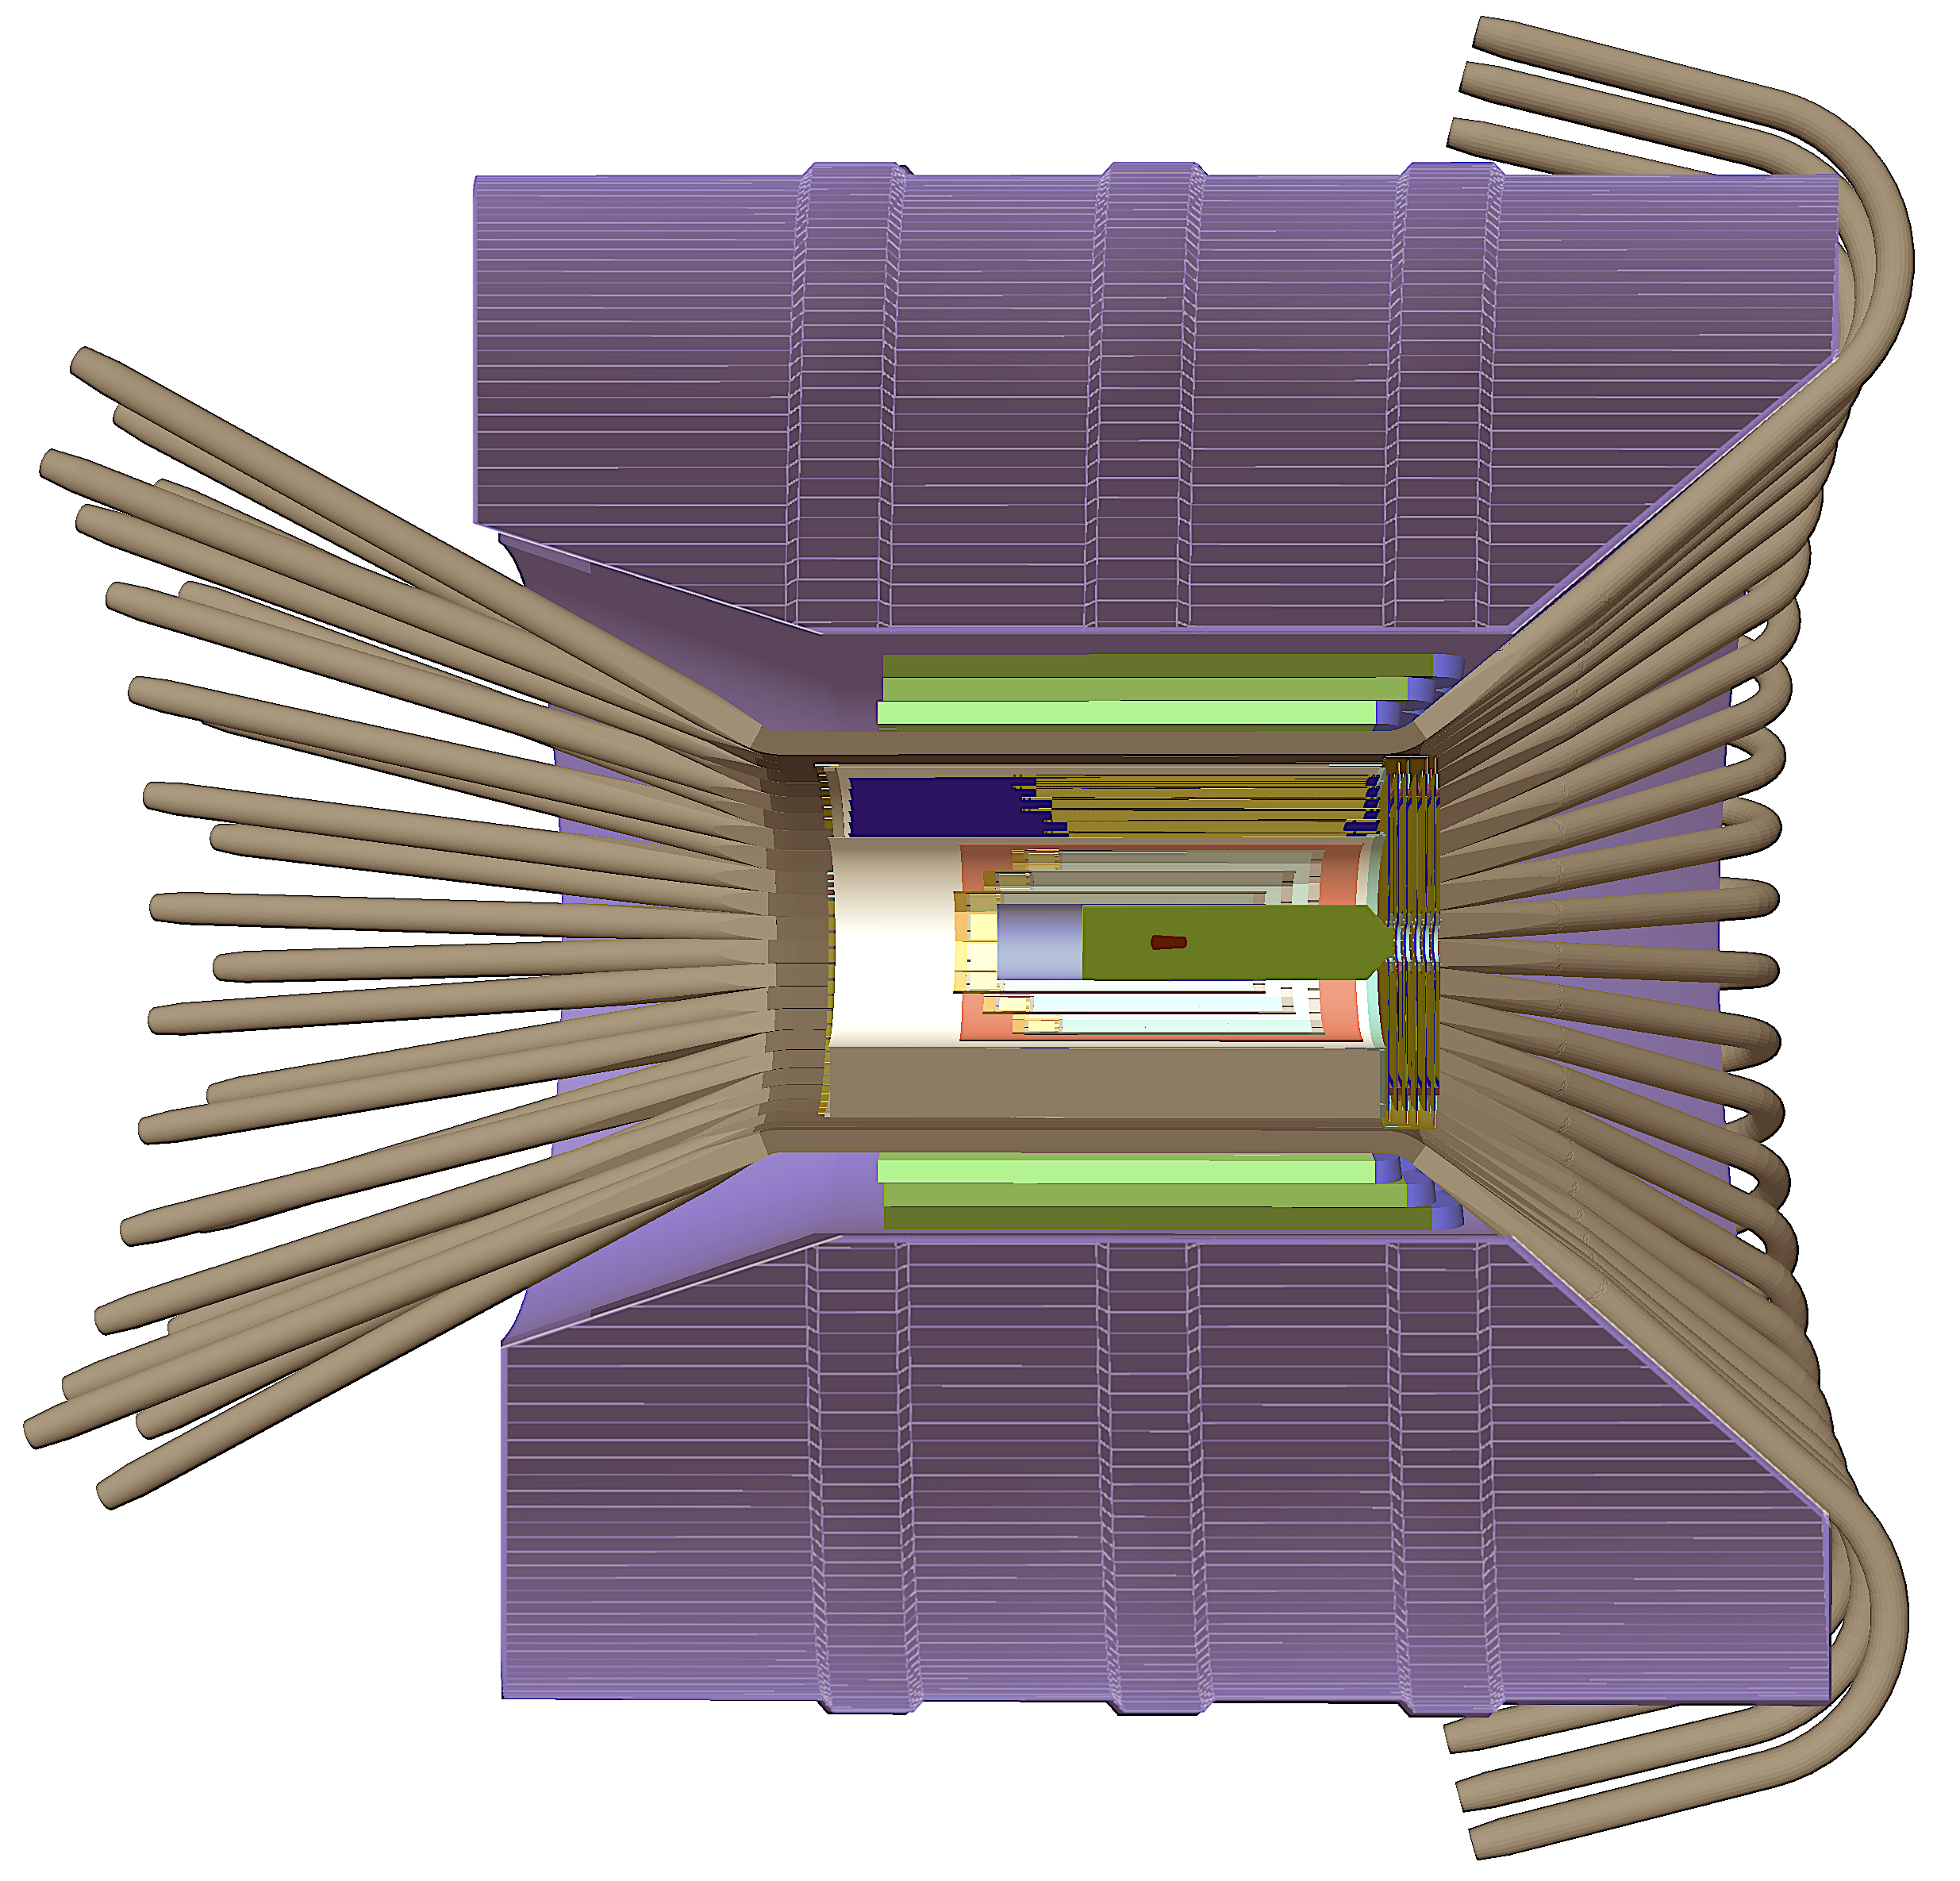
\includegraphics[width=0.99\columnwidth,keepaspectratio]{img/solenoid.png}
    \caption{(Color Online) The solenoid volume surrounding the CLAS12 Central Detector.}
	\label{fig:solenoid}
\end{figure}

The torus geometry is imported from the engineering CAD model through 54 tessellated volumes. Among the volumes are:

\begin{itemize}
	\item the bore heat shield and hub components
	\item the back and front hub steel plates
	\item the stainless steel coil vacuum jackets
	\item the torus coils containing the conductors, represented by copper volumes in Geant4
	\item internal shielding around the hub, made by tungsten cylinders (blue in \F{torus})
\end{itemize}

The torus hub is protected from the beampipe background with additional tungsten shielding.
The torus geometry is shown in \F{torus}.

\begin{figure}
	\centering
	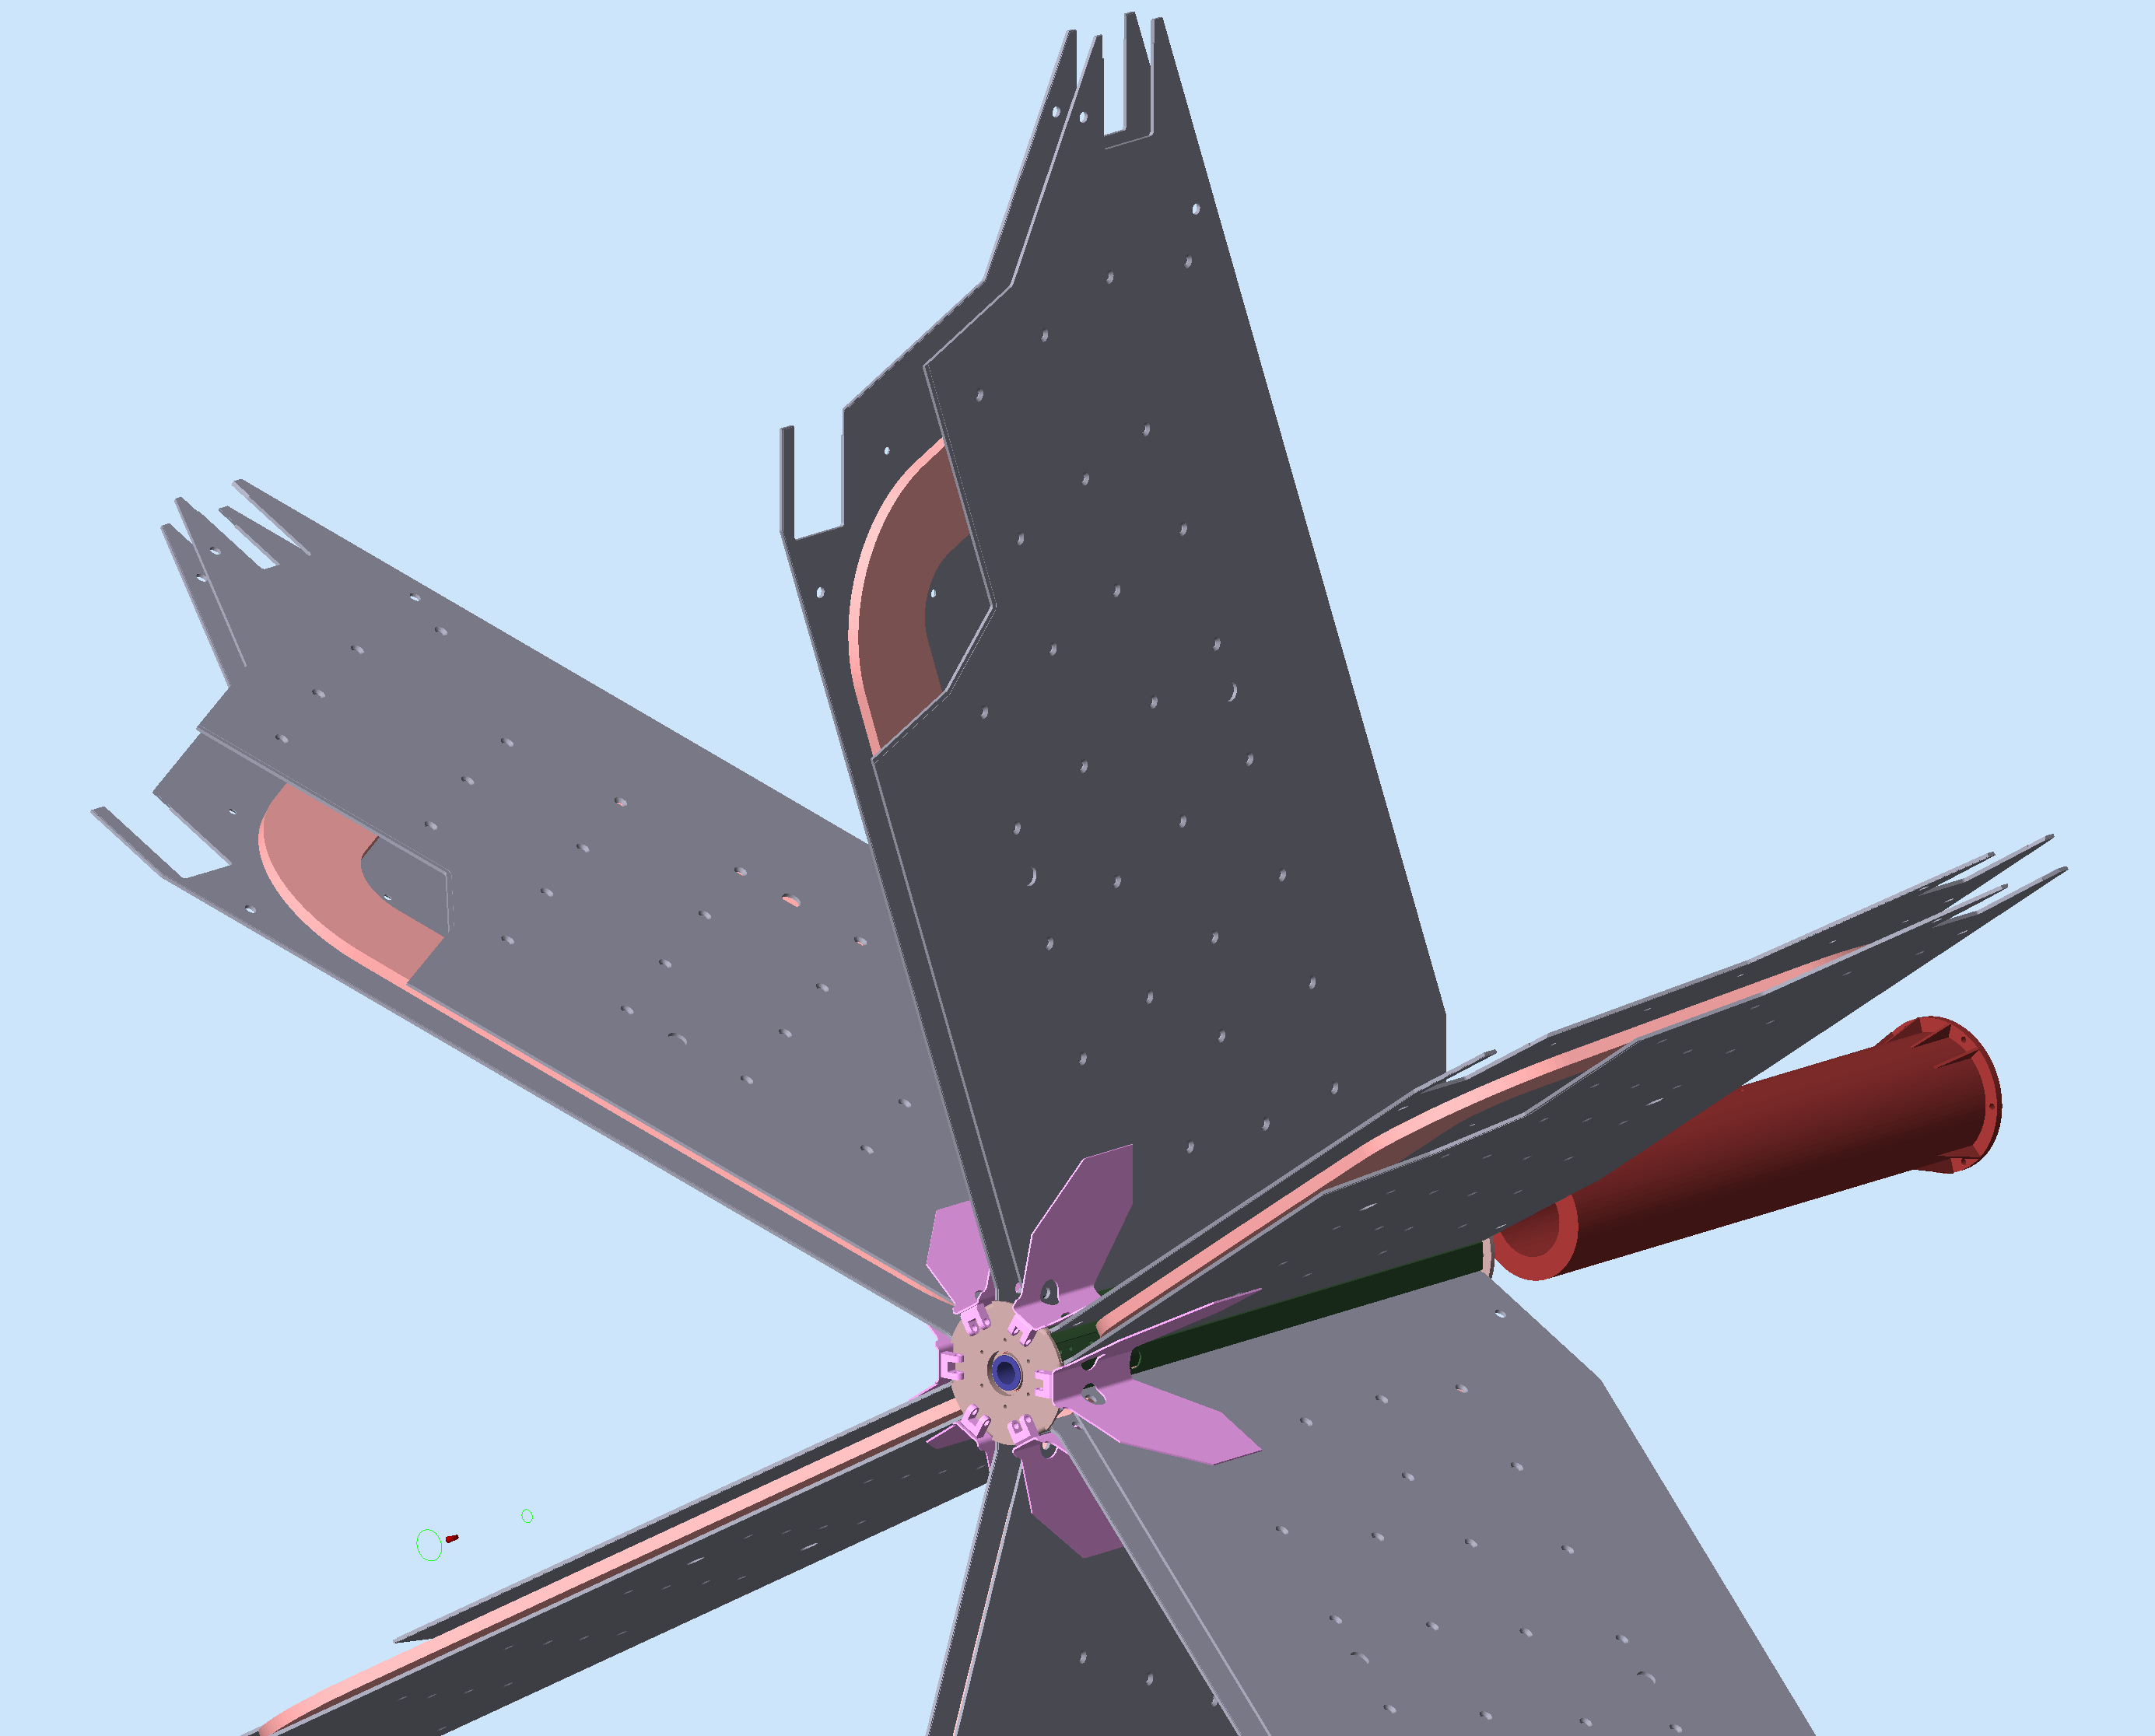
\includegraphics[width=0.99\columnwidth,keepaspectratio]{img/torusGeometry.png}
	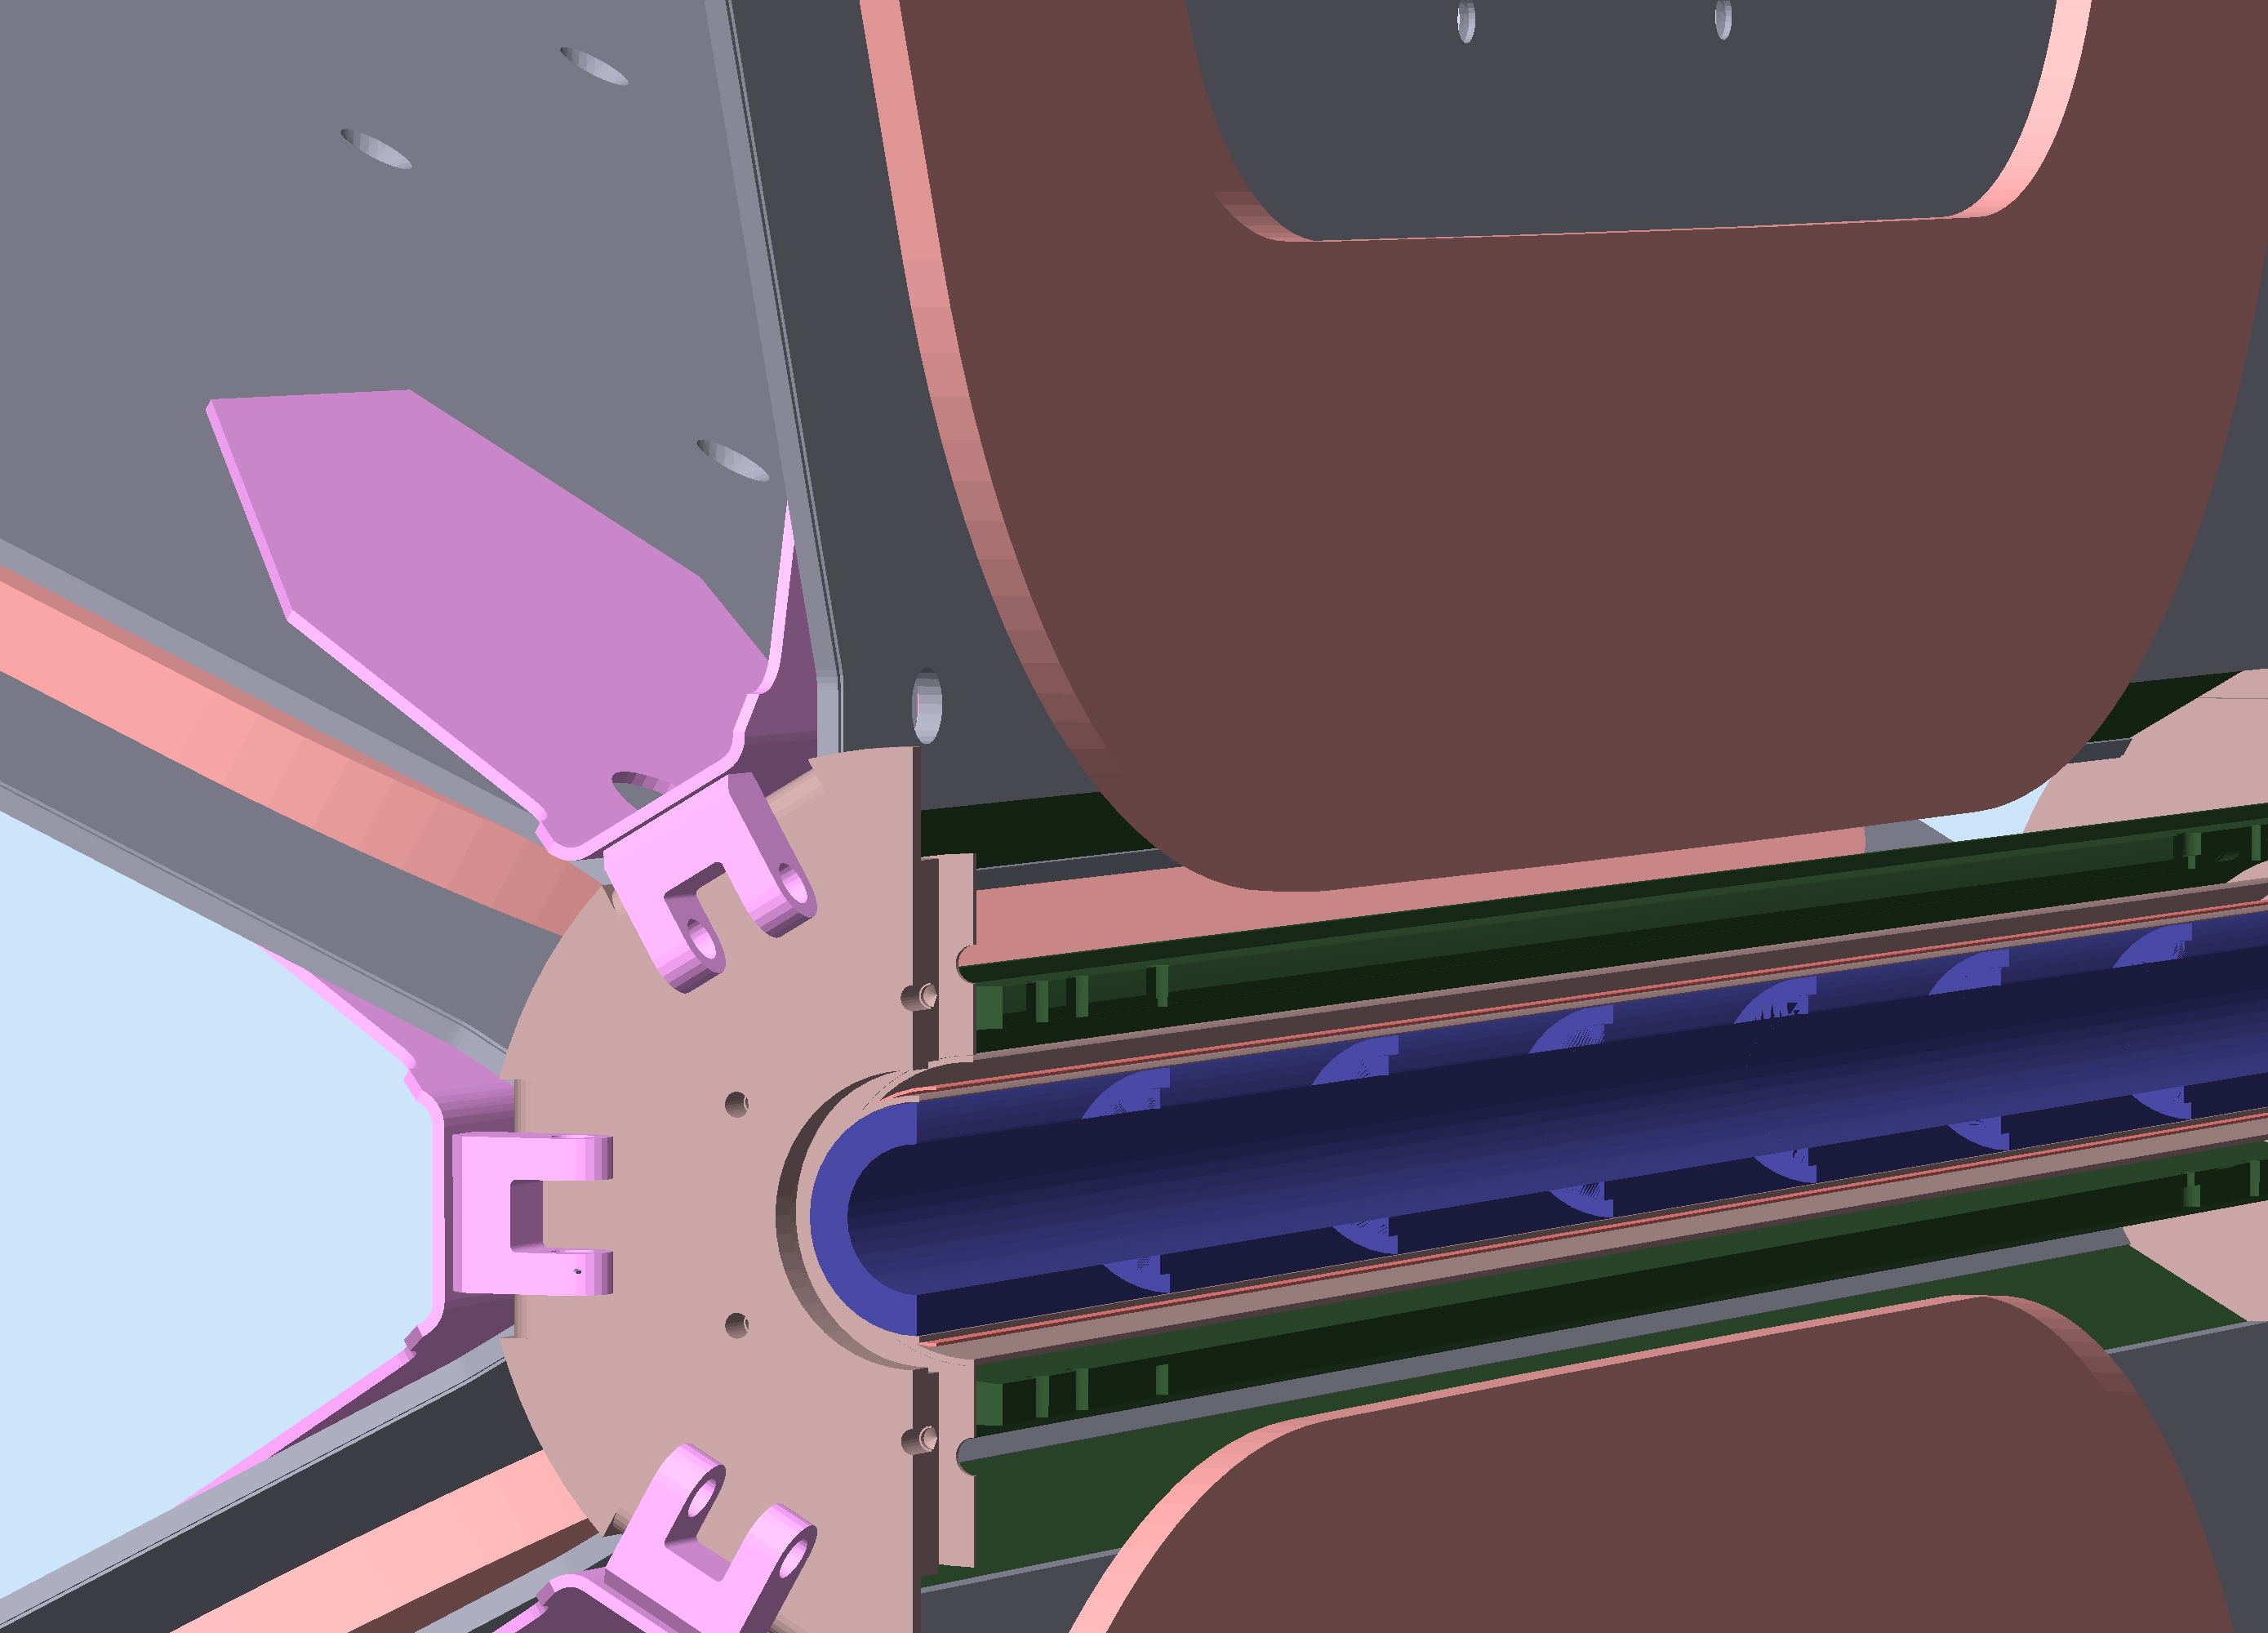
\includegraphics[width=0.99\columnwidth,keepaspectratio]{img/torusDetail.png}
	\caption{(Color Online) Top: the GEMC implementation of the torus hardware. The volumes are imported from the CAD engineering model.
             The stainless steel vacuum jacket embeds the Geant4 coil volumes.
			 Bottom: a section view of the torus in the vicinity of the beamline. The warm and cold hubs are visible, along with the
			 tungsten shielding in the innermost part of the hub.}
	\label{fig:torus}
\end{figure}


\subsubsection{Magnetic Field Maps} \label{clas12FieldMaps}

The CLAS12 torus and solenoid field maps are imported into the simulation using ascii files. Both fields can be scaled by an arbitrary factor.
Both fields are defined in the Hall-B coordinate system and both can be shifted and tilted by additional delta amounts.

\subsubsection{Solenoid}
The solenoid field map has cylindrical symmetry around the $z$-axis, so the map used in the simulation is defined
in the transverse / longitudinal plane and then rotated when requested by the Geant4 navigation.
The integration method used in the simulation is the fourth order Runge-Kutta technique \cite{rungeKutta}.

The solenoid field near the target is parallel to the $z$-axis and its uniformity was measured to be 318 ppm over a 25 mm
diameter and 40 mm long cylindrical volume. The field map grid is made by 600 points in the transverse coordinate,
from 0 to 3 m and by 1200 points along the $z$-axis, from \mbox{-3 m} to 3 m.
The field grid values are linearly interpolated to the $(x,y,z)$ coordinate requested by Geant4.
Table \ref{tab:solMap} shows the field map ascii data structure. The simulation of one event in a 250 ns time window at
the CLAS12 luminosity with and without solenoid magnetic field is presented in \F{solenoidONOFF}, showing the effectiveness
of the solenoid in providing electromagnetic shielding to M\"oller electrons.

\begin{table}[h]
	\begin{center}
		\begin{tabular}{| c | c | c | c |}
			T (m)  & Z (m) &  $B_T$ (T) & $ B_L (T)$ \\
			\hline
          0.005  &  -0.025 & 0.000013  & 5.000880 \\
          0.005  &  -0.020 & 0.000044  & 5.000822 \\
          0.005  &  -0.015 & 0.000073  & 5.000704 \\
          0.005  &  -0.010 & 0.000101  & 5.000529 \\
          0.010  &  -0.025 & 0.000028  & 5.000928 \\
          0.010  &  -0.020 & 0.000089  & 5.000867 \\
          0.010  &  -0.015 & 0.000148  & 5.000747 \\
          0.010  &  -0.010 & 0.000203  & 5.000570 \\
		\end{tabular}
	\end{center}
\caption{Solenoid ascii field map values around the target. T is the transverse coordinate $\sqrt{(x^2+y^2)}$ and $z$ is the longitudinal coordinate.
		 The solenoid field is centered at $z=0$, the location of the center of the target.}\label{tab:solMap}
\end{table}

\begin{figure}
	\centering
	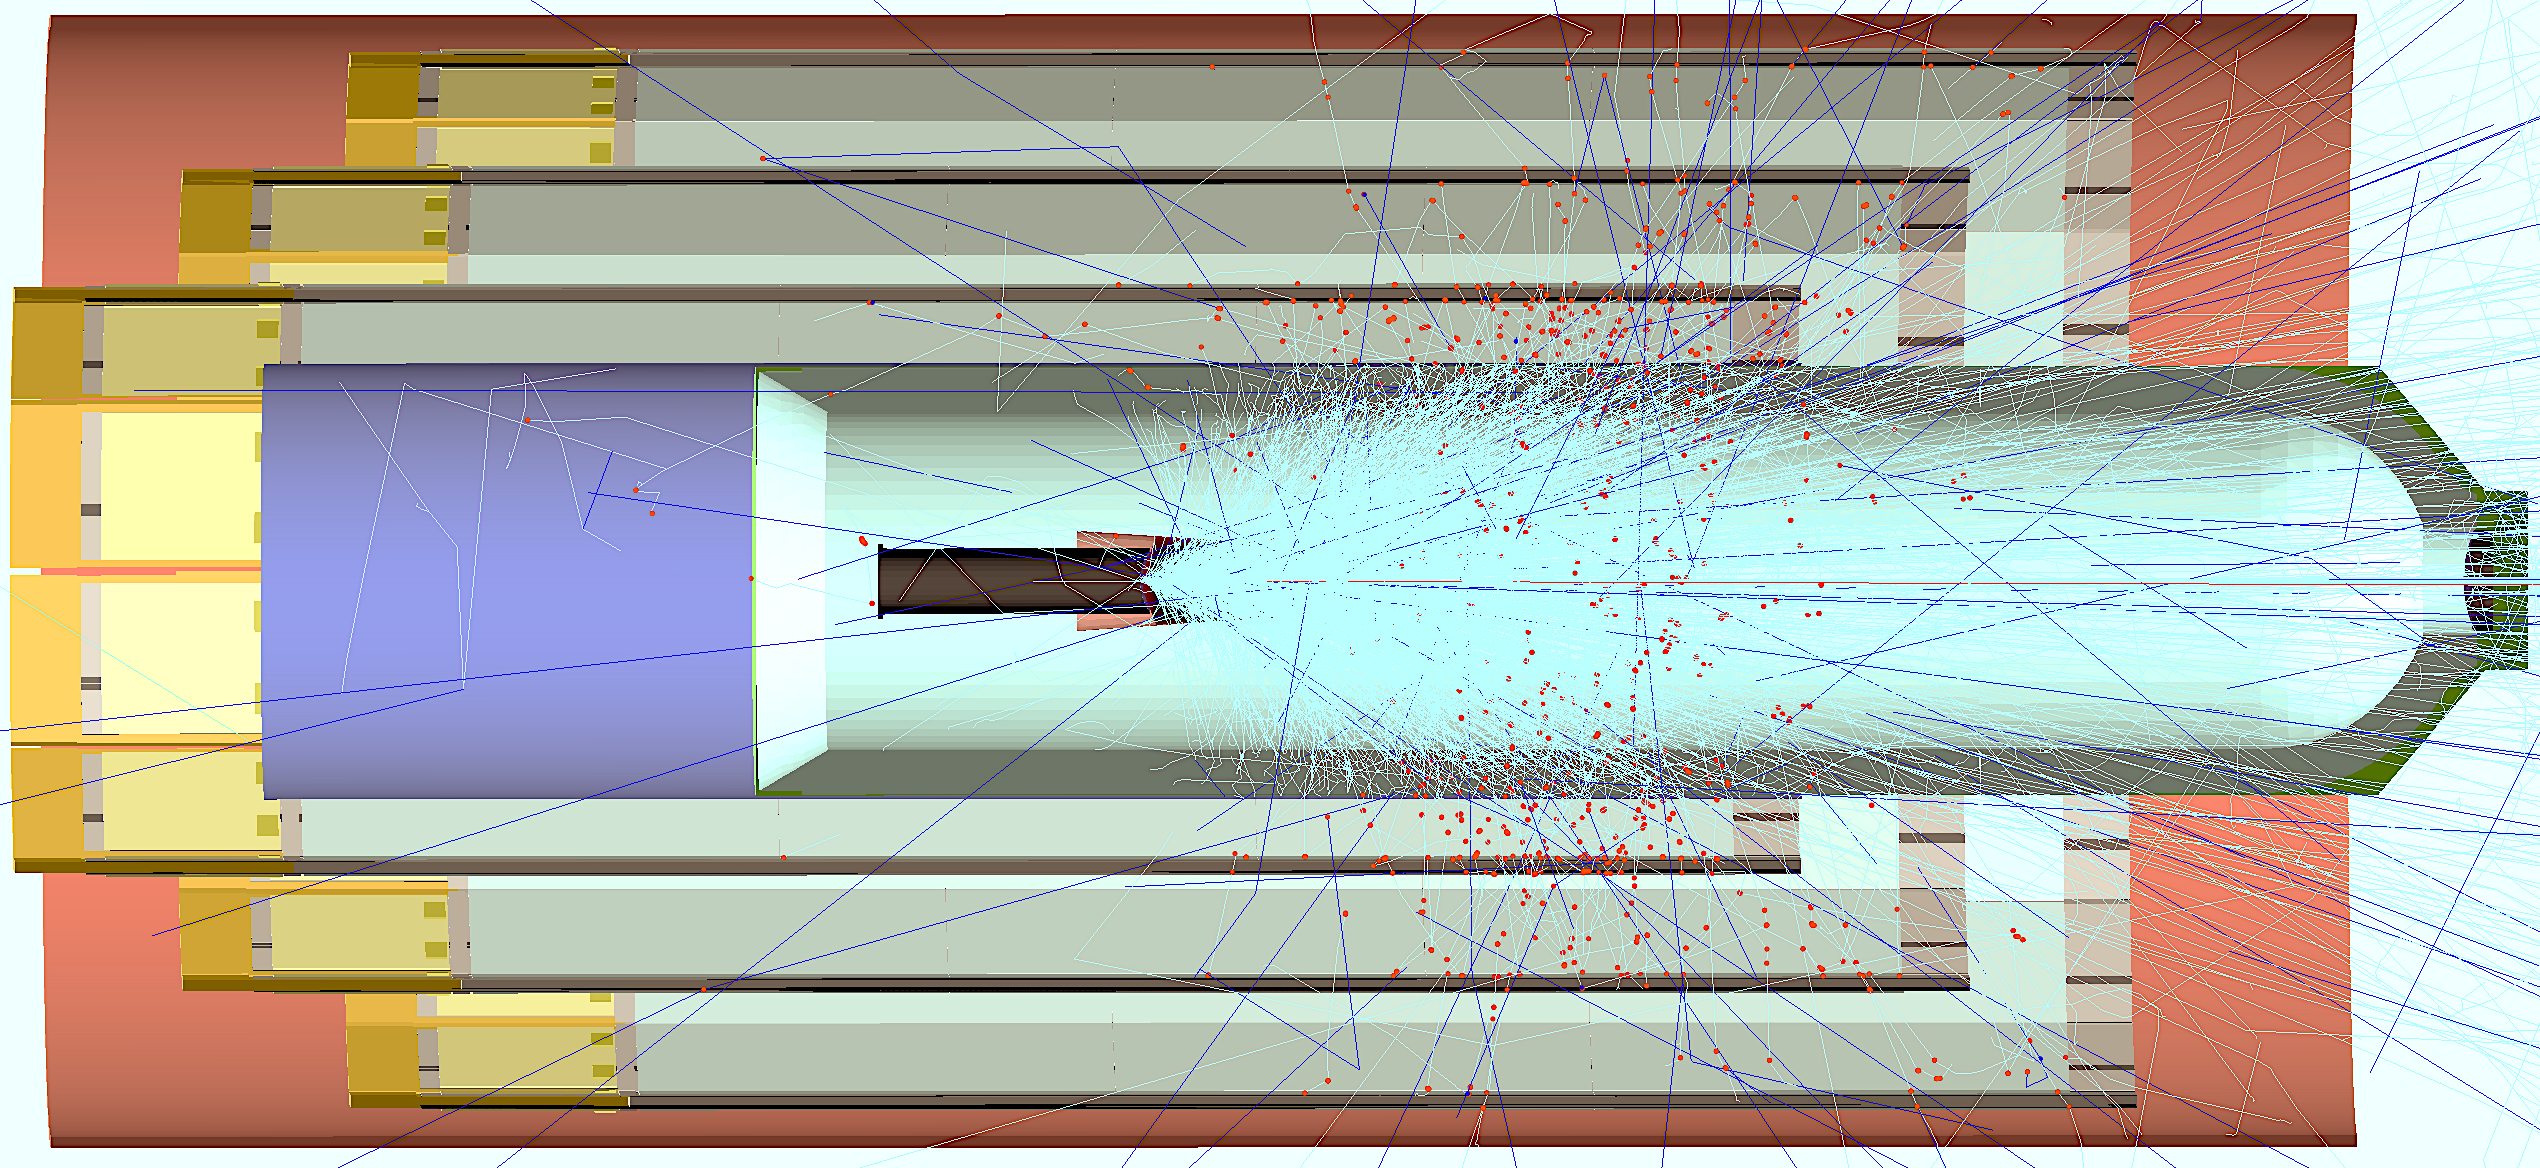
\includegraphics[width=0.98\columnwidth,keepaspectratio]{img/solenoidOFF.png}
	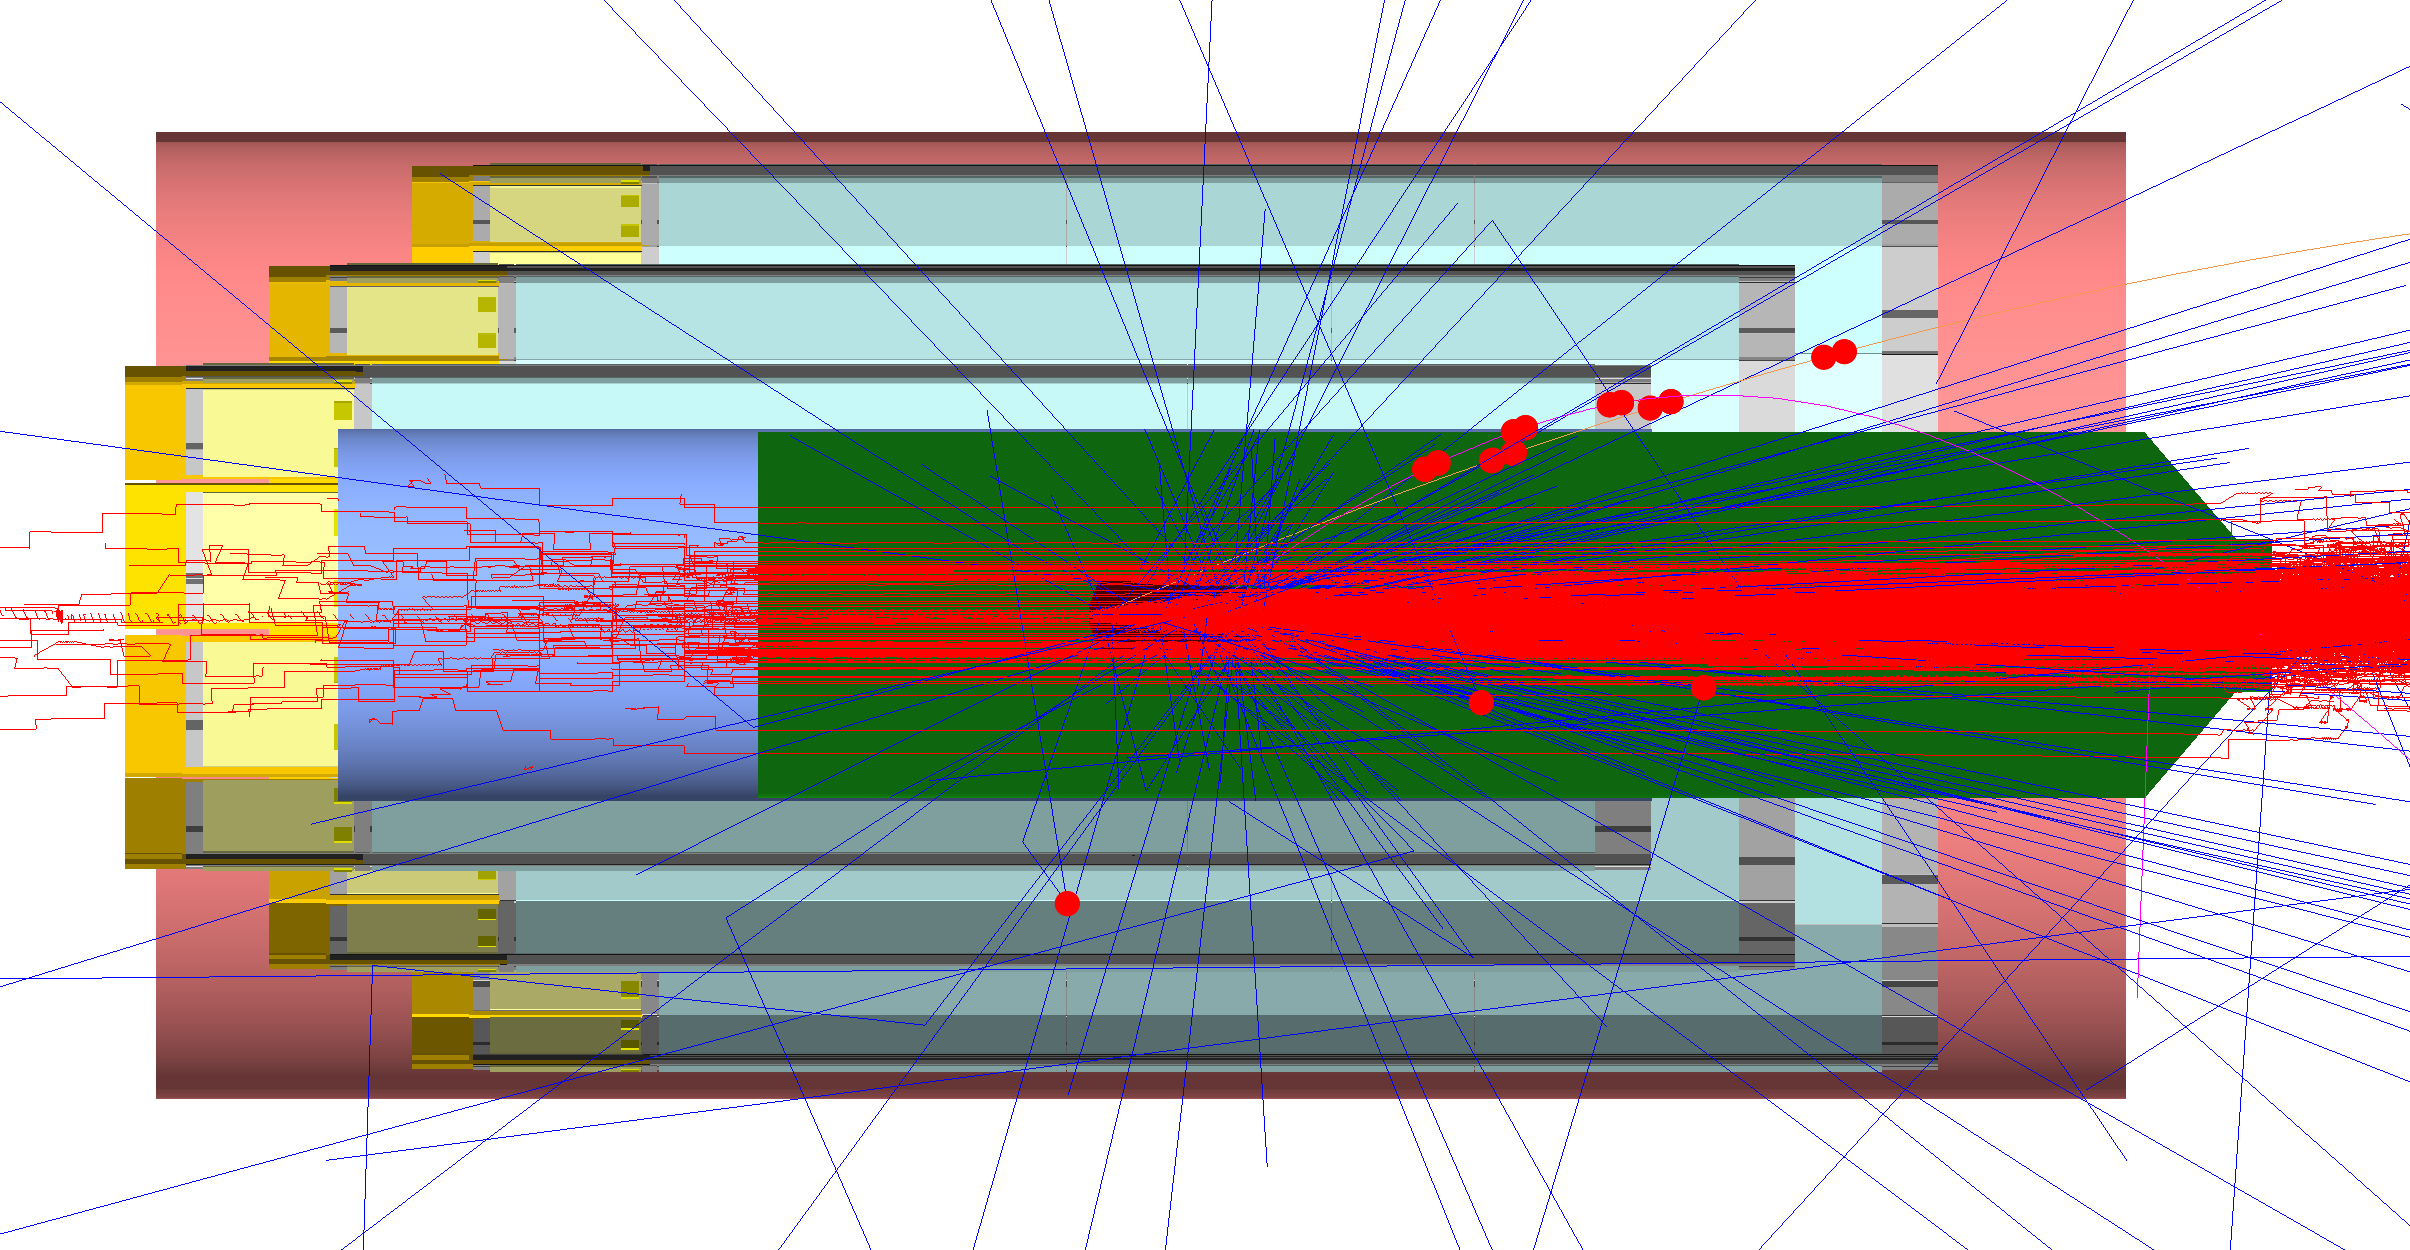
\includegraphics[width=0.98\columnwidth,keepaspectratio]{img/solenoidON.png}
    \caption{(Color Online) An 11 GeV electron beam impinges on a 5-cm long liquid-hydrogen target. The SVT detector is shown.
             At the full 10$^{35}$ cm$^{-2}$ s$^{-1}$ luminosity, this correspond to 124,000 electrons in a 250 ns time window.
			 Top: no solenoid field. One full luminosity event in a 250 ns time window produce a storm of M\"oeller electrons that
             saturates the SVT. Each red point is a recorded hit above the SVT threshold.
			 Bottom: full solenoid field. One full luminosity event in a 250 ns time window.
             The solenoid focuses all of the M\"oeller electrons along the beamline, providing an effective electromagnetic shield for CLAS12.
			 The only hits above threshold are the ones generated by real hadronic tracks. }
	\label{fig:solenoidONOFF}
\end{figure}

\subsubsection{Torus}
The torus field can be imported using a symmetric map or a full 3D map.
The symmetric map is defined in half of a CLAS12 sector. It is symmetric around the sector mid-plane and copied in each sector
when requested by the Geant4 navigation. The 3D map covers the entire cartesian space and accounts for field deviations due to coil
movements or imperfections \cite{GhoshalSolenoid}.

The field map has 251 points along the $z$-axis, from 1 m to 3 m. It has 2501 points in the transverse coordinate, from 0 to 5 m.
It has 16 azimuthal points from 0\mdeg to 30\mdeg. The field grid values are linearly interpolated to the $(x,y,z)$
coordinate requested by Geant4.

The torus field in the sector mid-plane is perpendicular to the $z$-axis and is typically $2.058$ T.
Table \ref{tab:torMap} shows the field map ascii data structure.

\begin{table}[h]
	\begin{center}
		\begin{tabular}{| c | c | c | c | c | c | }
         $\phi$ (deg) & T (m)    & Z (m)    &  $B_x$  &    $B_y (T)$    & $B_z$\\
			\hline
          0.0         &  190.0   &  338.0   &  0       &     0.451275 &  0 \\
          0.0         &  190.0   &  340.0   &  0       &     0.450136 &  0 \\
          0.0         &  190.0   &  342.0   &  0       &     0.448789 &  0 \\
          0.0         &  190.0   &  344.0   &  0       &     0.447235 &  0 \\
          0.0         &  190.0   &  346.0   &  0       &     0.445472 &  0 \\
          0.0         &  190.0   &  348.0   &  0       &     0.443502 &  0 \\
          0.0         &  190.0   &  350.0   &  0       &     0.441323 &  0 \\
          0.0         &  190.0   &  352.0   &  0       &     0.438935 &  0 \\
		\end{tabular}
	\end{center}
	\caption{Torus ascii field map values near mid-sector. T is the transverse coordinate $\sqrt{(x^2+y^2)}$ and
             $z$ is the longitudinal coordinate.}
 	\label{tab:torMap}
\end{table}


The Github location of the GEMC perl API script for the solenoid and the torus CAD volumes is \url{https://github.com/gemc/detectors/tree/master/clas12/magnets}.


\subsection{Beamline}

The CLAS12 beamline downstream of the target is made up of several pieces, each discussed below. The positioning and composition of the beamline
depends on the run configuration, that can be:

\begin{itemize}
	\item FTOn: Forward Tagger present and operational. The Moller shield starts at z=877 mm from the target center to, see \F{beamlineGeometry} top.
	\item FTOff: FT is present but not operational. The FT tracker is replaced by shielding.
                 The Moller shield starts at z=430 mm from the target center, and additional shielding is present to connect it to the FT. See, \F{beamlineGeometry} bottom.
\end{itemize}


\begin{figure}
	\centering
	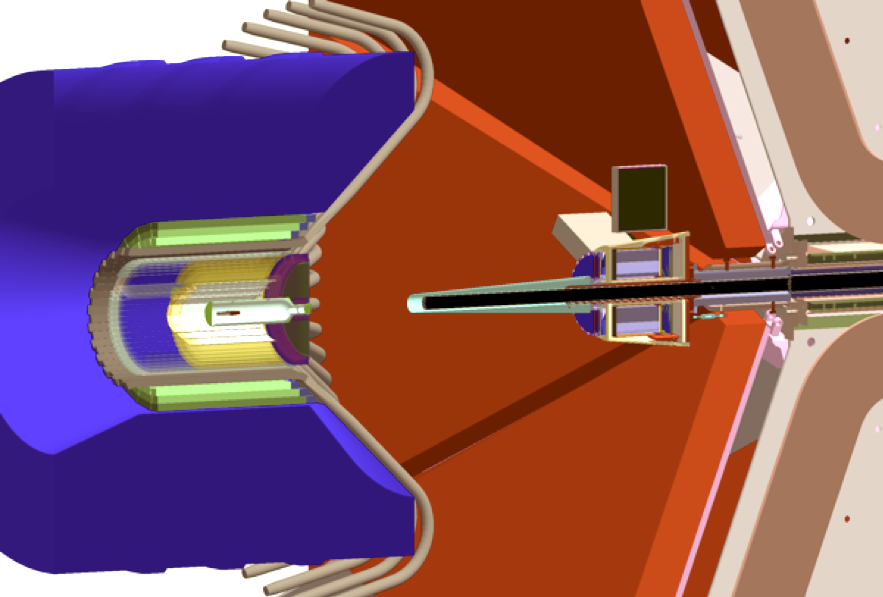
\includegraphics[width=0.98\columnwidth,keepaspectratio]{img/ftOnGeometry.png}
	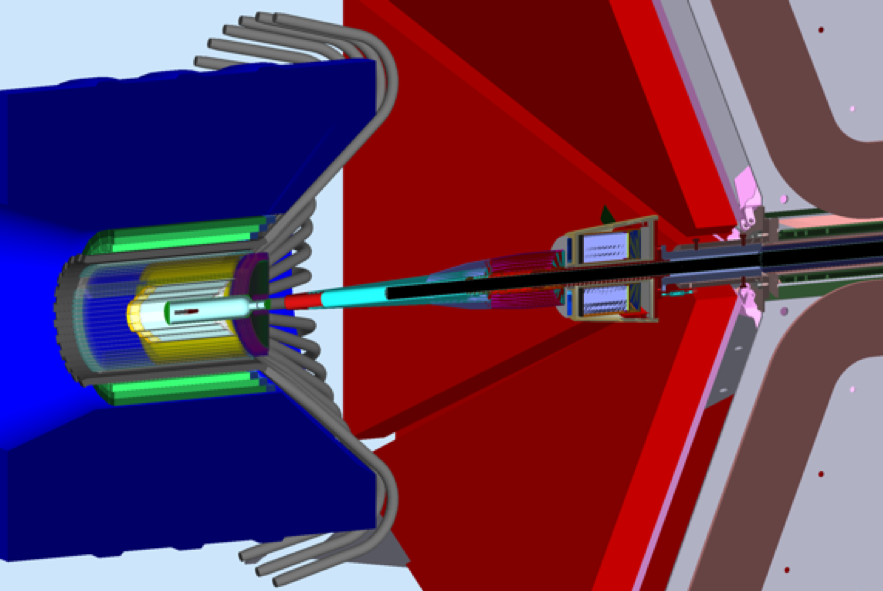
\includegraphics[width=0.98\columnwidth,keepaspectratio]{img/ftOffGeometry.png}
   \caption{The two possible CLAS12 configurations. Top: FTOn. To clear its acceptance at forward angles ($2.50-4.50$ degrees)
            the Moller shield (cyan color) is attached to the FT tracker, starting at $z=877$ mm from the target.
            Bottom: FToff; the FT is present but not operational. The FT tracker is replaced with a shield.
            The Moller cone is placed at $z=430$ mm from the target and additional shielding minimize background in Region 1 Drift Chambers.}
	\label{fig:beamlineGeometry}
\end{figure}

\subsection{Vacuum pipe}

A stainless steel vacuum pipes that contain the electron beam. The pipe starts downstream of the target at $z=80cm$
and changes dimensions inside the torus and downstream of the torus as detailed in Table \ref{tab:beampipe}

\begin{table}[h]
	\begin{center}
		\begin{tabular}{| c | c | c |}
			\hline \hline
			                & Thickness (mm) & Inner Radius (mm)   \\
			\hline
              Upstream      &    1.6     &    26.9 \\
              Inside        &    1.6     &    33.3 \\
            Downstream      &    3.2     &    60.3 \\
			\hline \hline
		\end{tabular}
	\end{center}
	\caption{The vacuum pipe three dimensions sets (in mm) upstream, inside and downstream of the torus}\label{tab:beampipe}
\end{table}


\subsection{Moeller Shielding}
The Moeller shielding is composed of the following elements, shown in \F{moellerShieldingFTOn} for the FTOn configuration
and in \F{moellerShieldingFTOff} for the FTOff configuration.

\begin{figure}
	\centering
	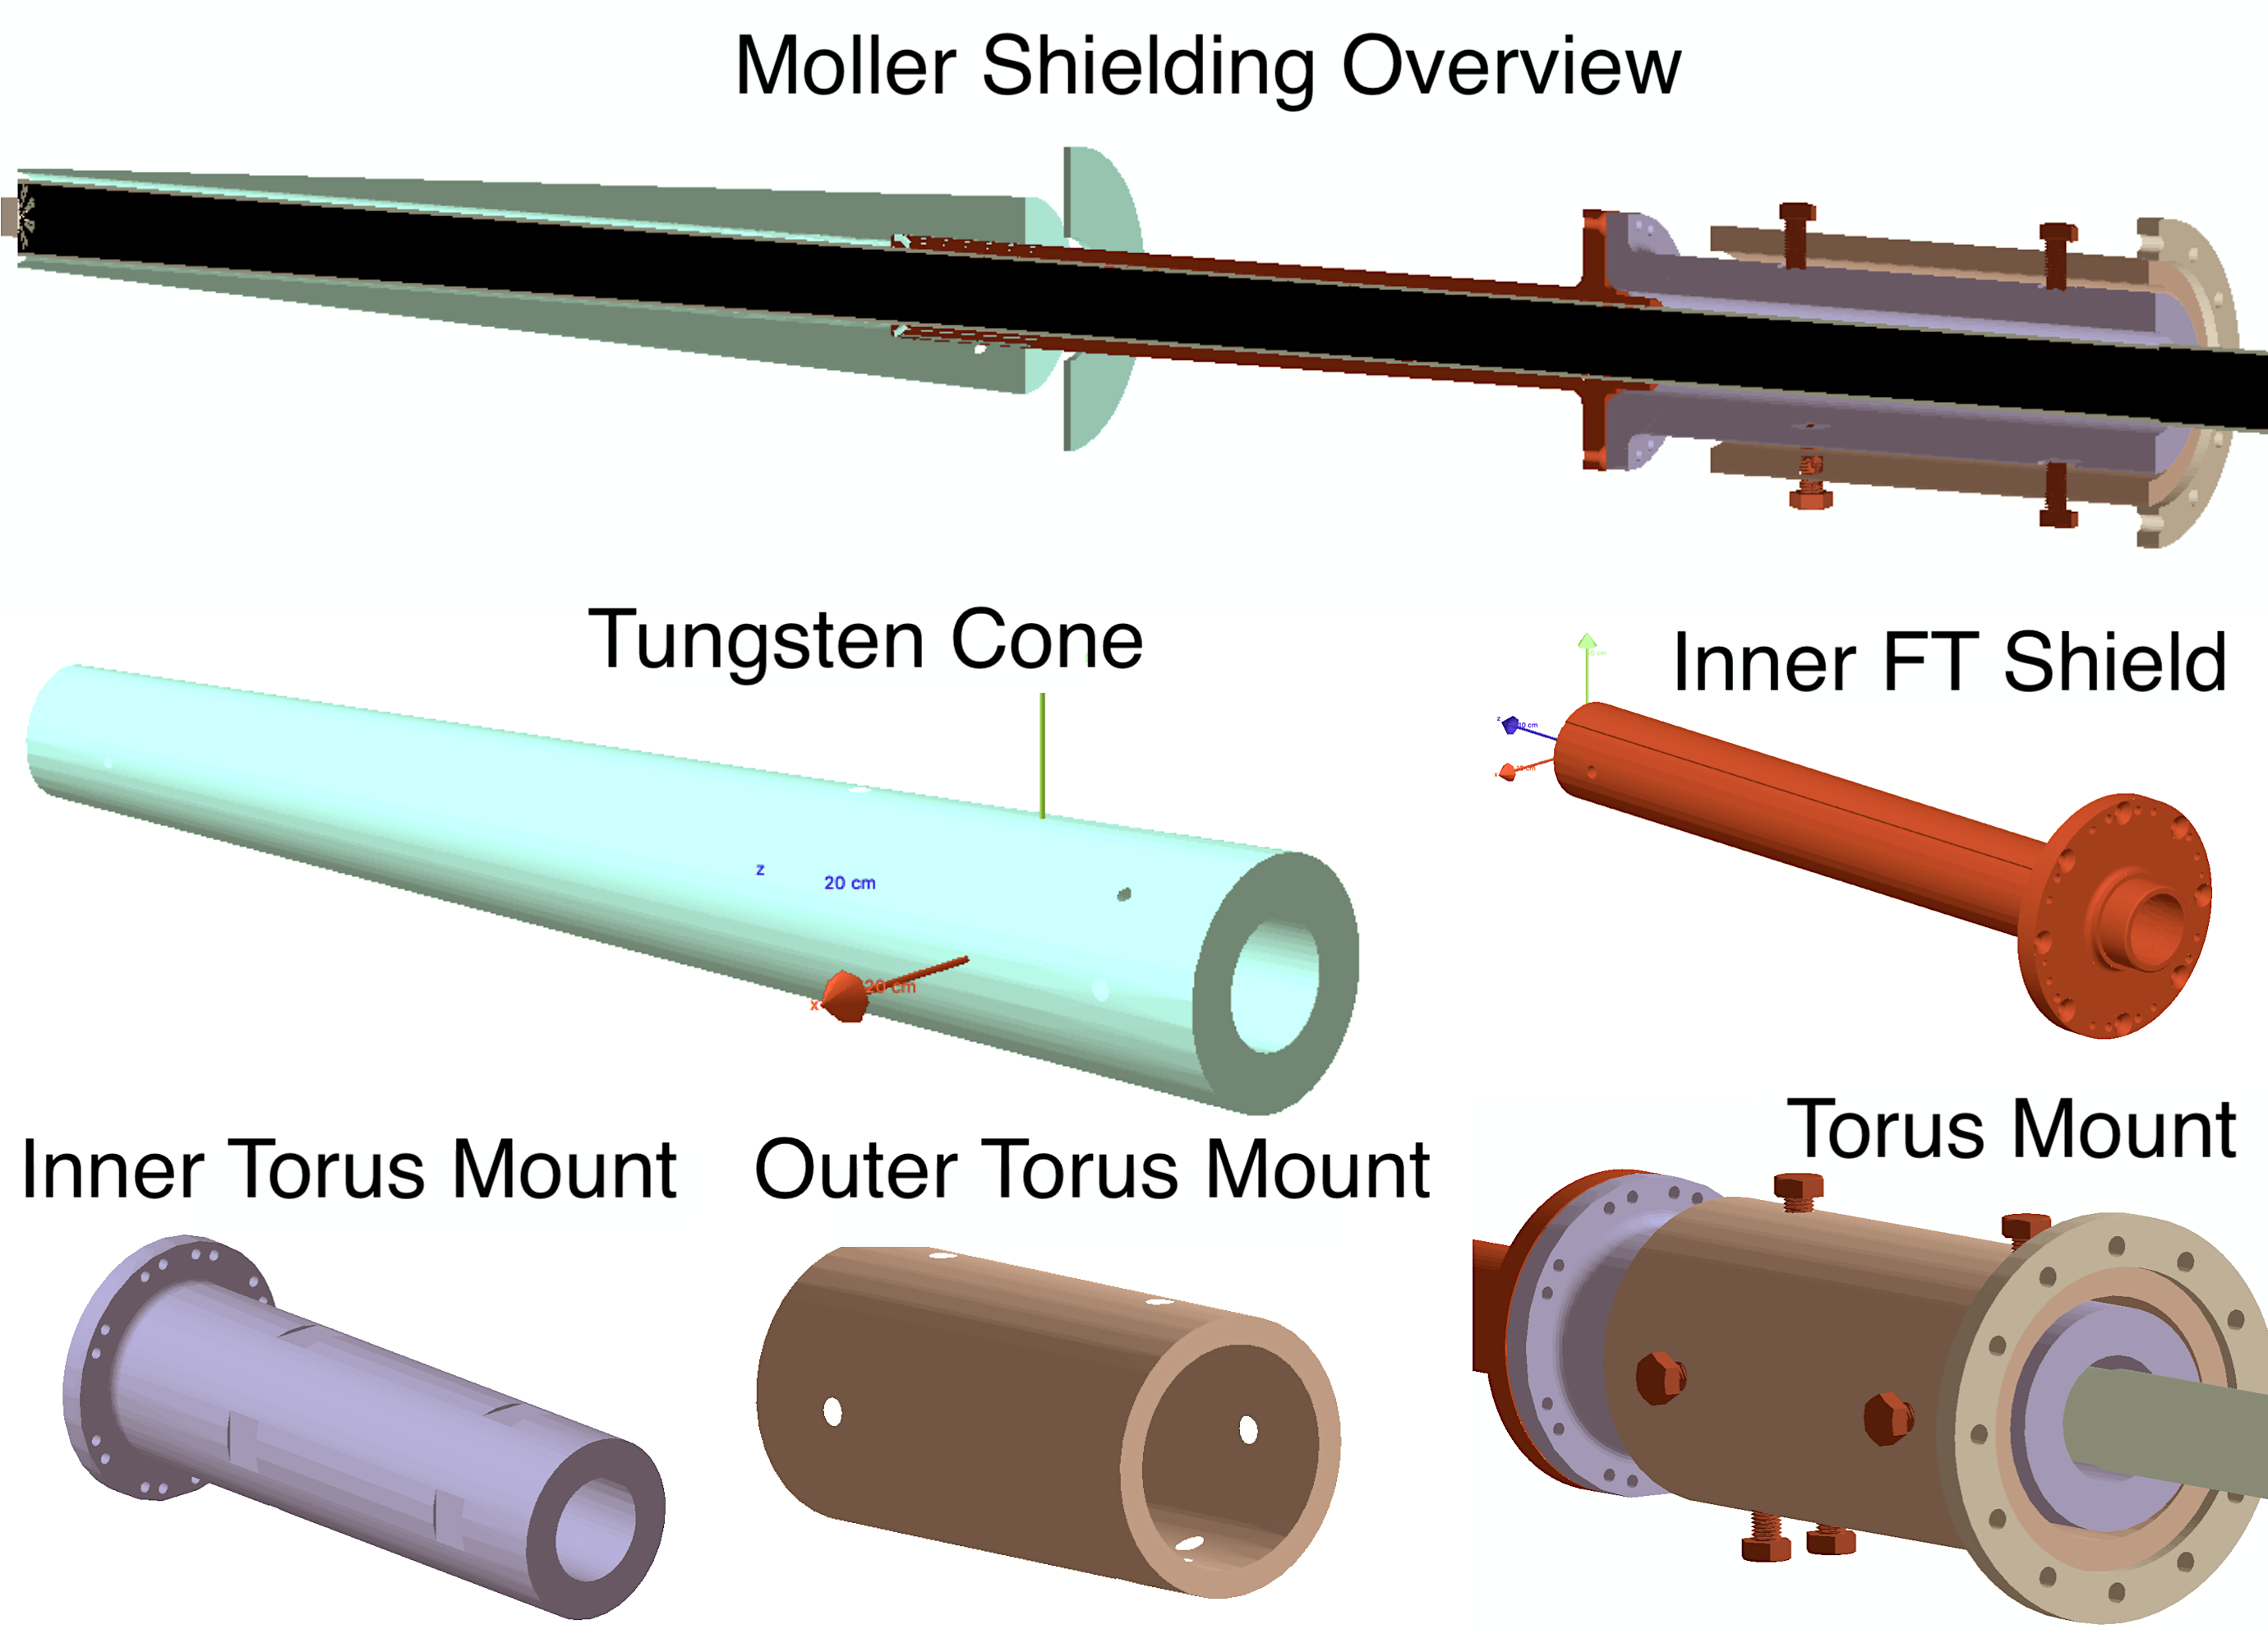
\includegraphics[width=0.98\columnwidth,keepaspectratio]{img/moellerShieldingFTOn.png}
	\caption{The Moeller shielding for the FT On configuration. Top: section of the overall overview of the cone, FT support and torus mount.
		     Various individual components are shown: the tungsten cone, the inner FT shield, and the structure of the torus mount.}
	\label{fig:moellerShieldingFTOn}
\end{figure}

\begin{figure}
	\centering
	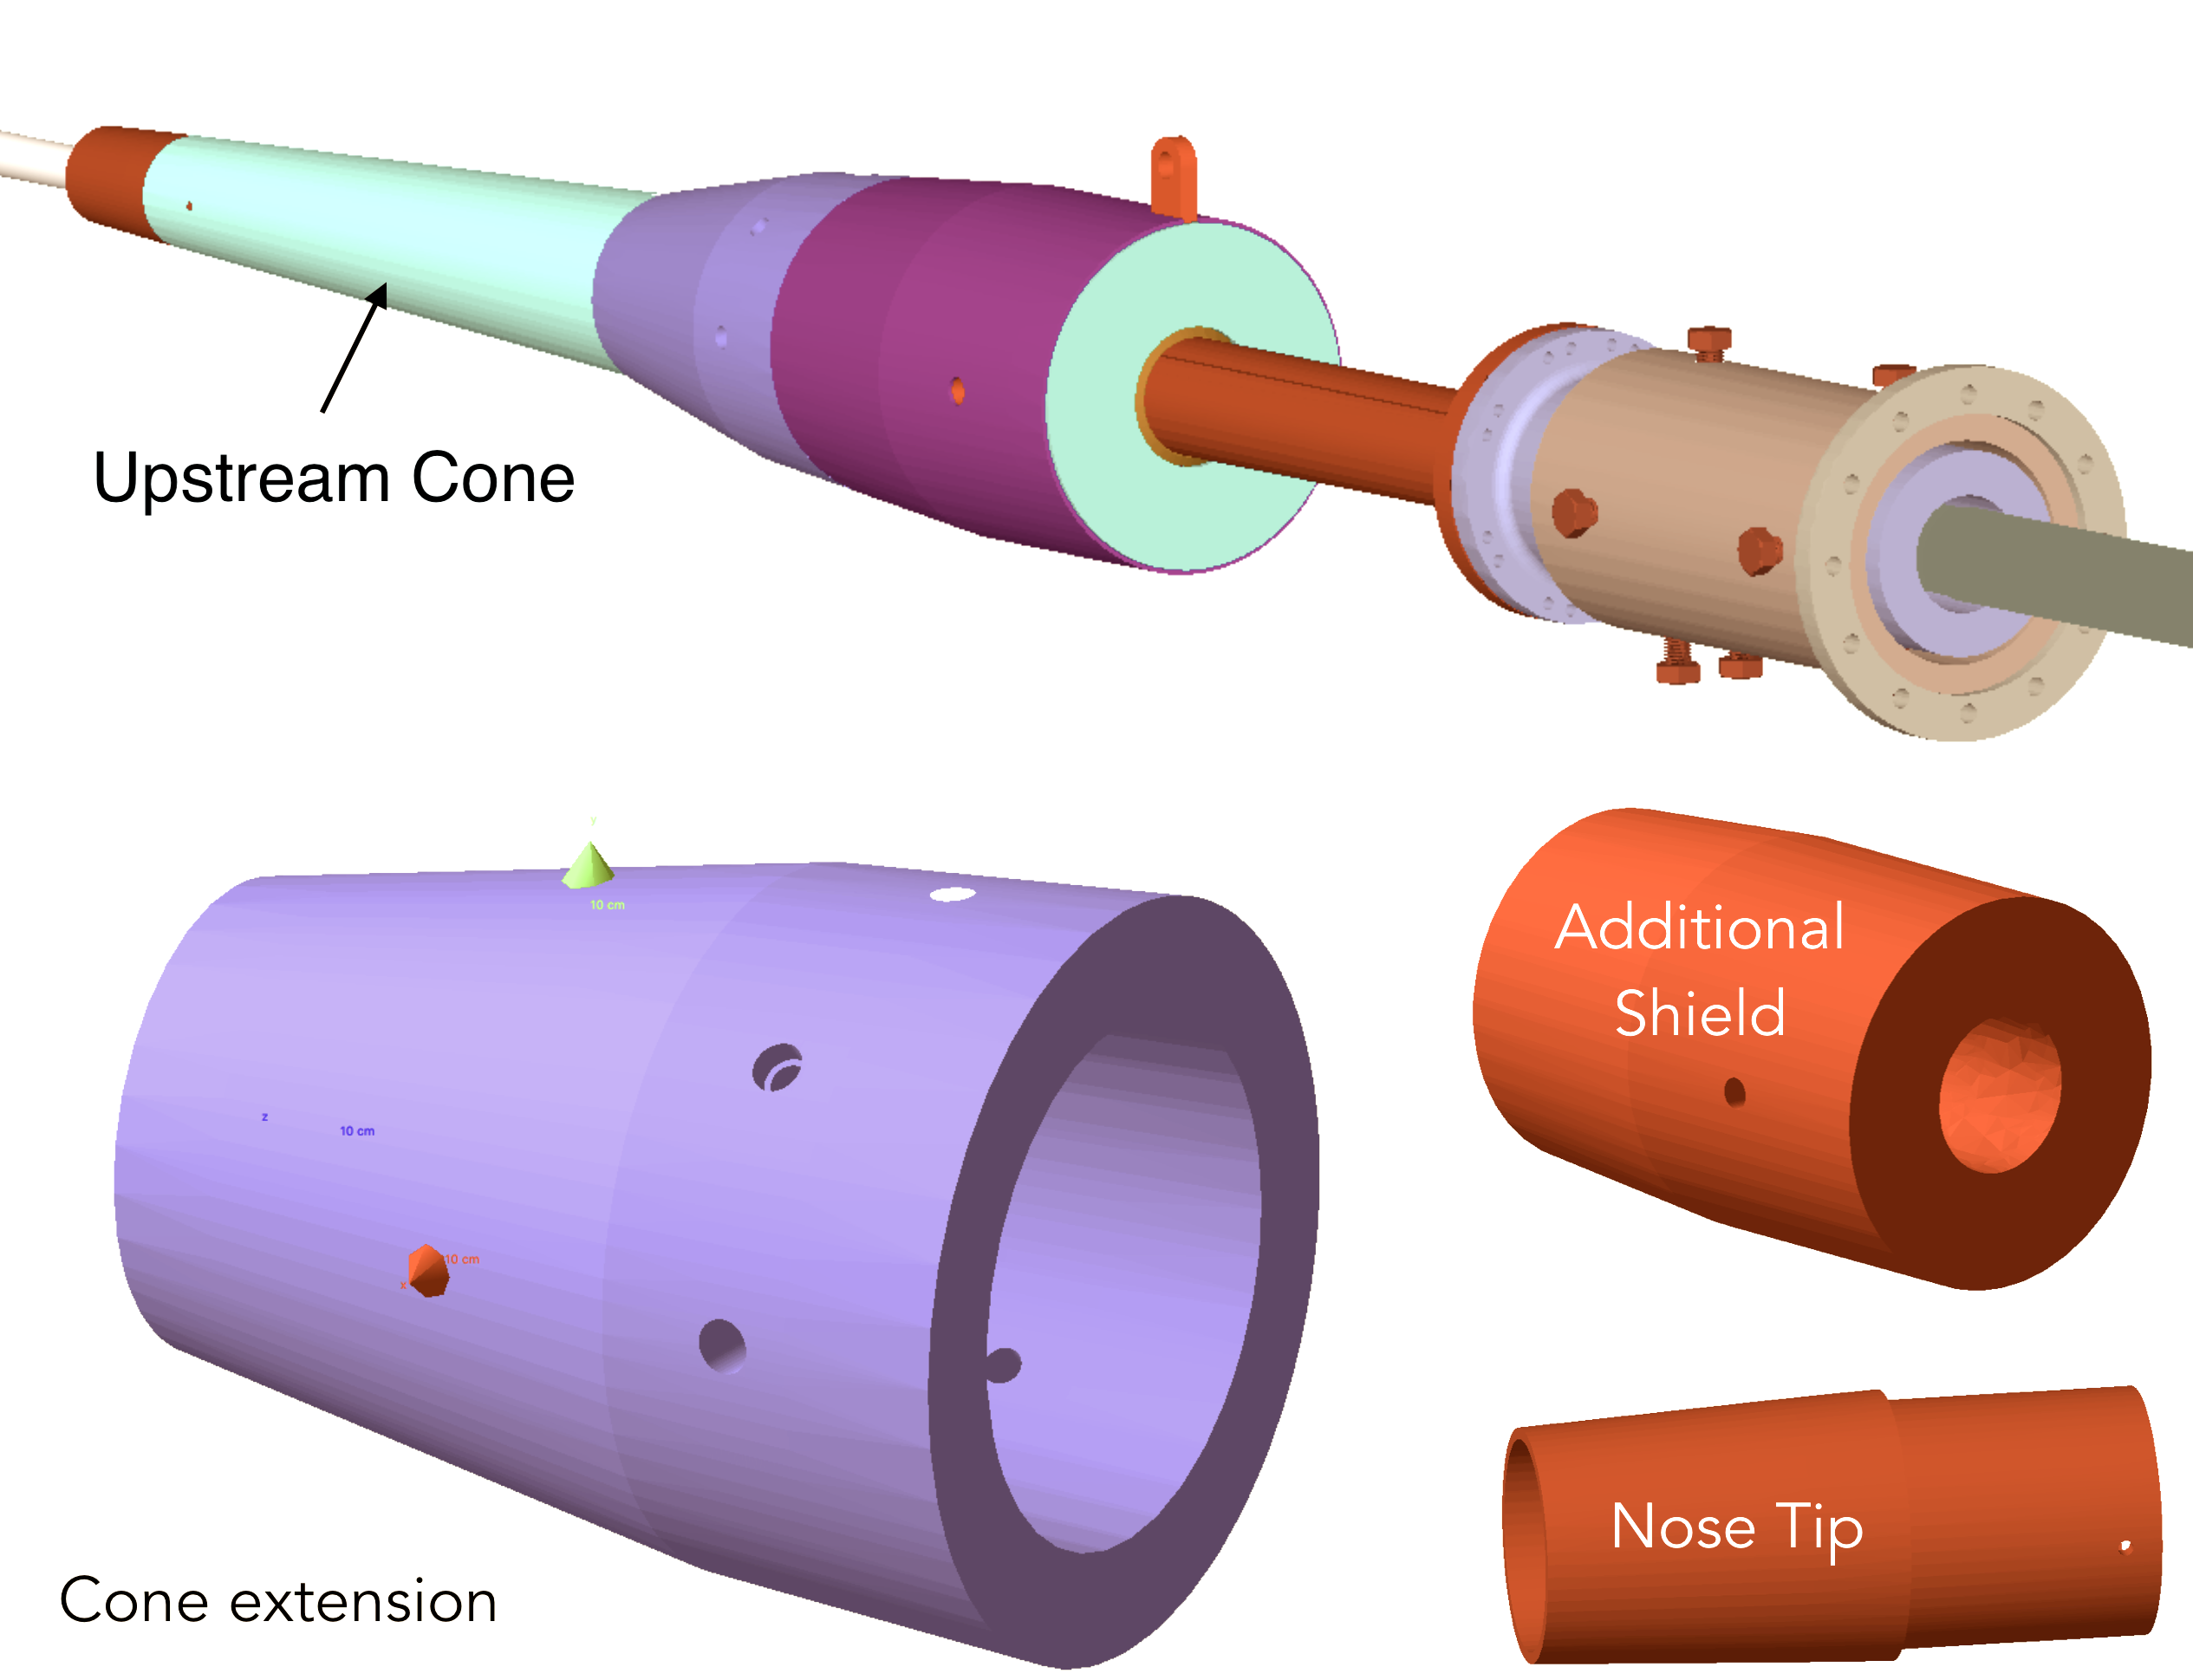
\includegraphics[width=0.98\columnwidth,keepaspectratio]{img/moellerShieldingFTOff.png}
   \caption{The Moeller shielding for the FT Off configuration. Top: section of the overall overview of the cone, FT support and torus mount.
            the cone tip extension and the additional shielding that replace the FT tracker is also shown.}
	\label{fig:moellerShieldingFTOff}
\end{figure}



\begin{itemize}
	\item FT On and FT Off configurations:
	\begin{itemize}
		\item a Tungsten cone with increasing thickness.
		\item a tungsten pipe and flange inside the FT
		\item a support system to mount the FT and the shielding onto the torus frame, composed by:
		\begin{itemize}
			\item an inner stainless steel shield and flange
			\item an outer tungsten shield
			\item nine copper screw to adjust the alignment of the FT and shields upstream of the torus
		\end{itemize}
	\end{itemize}
	\item Additions for FT Off configuration:
	\begin{itemize}
	\item a Tungsten cone tip to extend the Moeller shield cone
	\item lead cylinder in place of the FT tracker
	\end{itemize}

\end{itemize}




\subsection{Torus and downstream Shielding}
Additional shielding is placed around the vacuum pipe inside the torus hub in the form of tungsten cylinders.
A shielding downstream of the torus in the form of a connecting tungsten nose and a long lead cylinder enclosed by a stainless steel frame.
These components are shown in \F{downstreamShielding}.

\begin{figure}
	\centering
	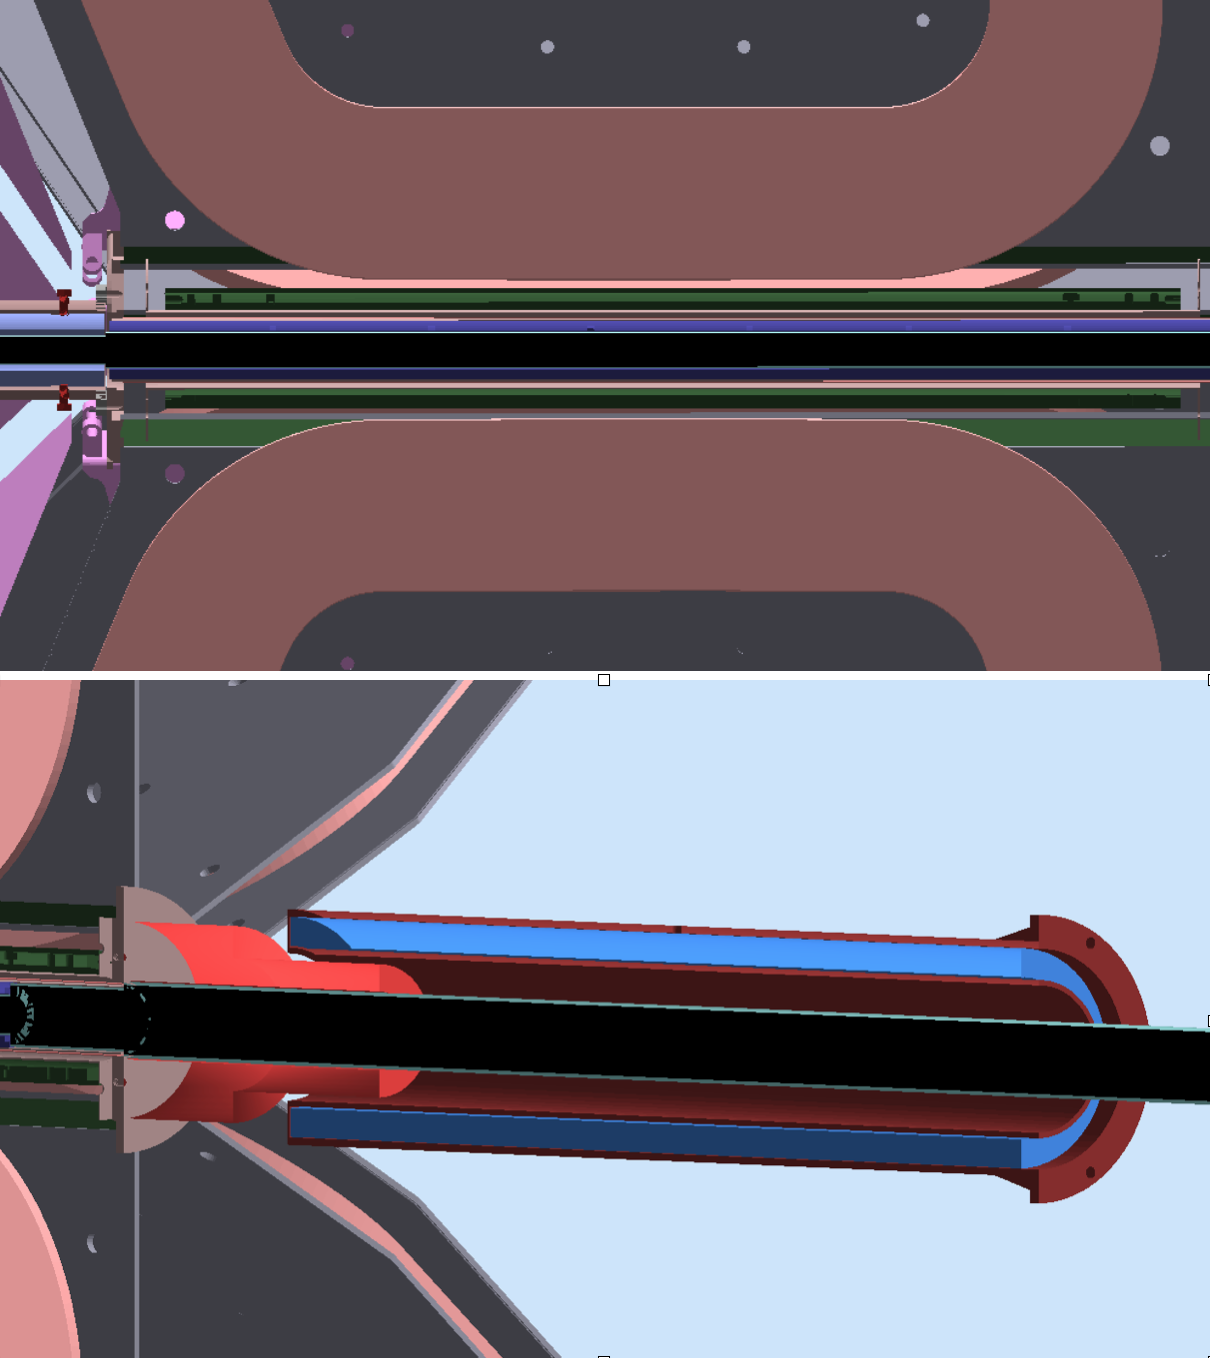
\includegraphics[width=0.98\columnwidth,keepaspectratio]{img/downstreamShielding.png}
	\caption{Torus and Downstream shielding. Top: several tungsten cylinders were placed around the vacuum line (bloe colors).
            Bottom: a long lead cylinder (blue) is enclosed by a stainless steel frame.}
	\label{fig:downstreamShielding}
\end{figure}



\subsection{Geometry Source}

The beamline geometry is entirely imported from the engineering CAD model.

The Github location of the GEMC geometry CAD volumes is \url{https://github.com/gemc/detectors/tree/master/clas12/cadBeamline}.

\subsection{Summary of Detector Parameters}

The CLAS12 detector parameters are summarized in Table~\ref{tab:summary}. For most of the detectors the
maximum step is set to a conservative 1 cm value. The actual step size in this case is decided by Geant4 using the
cross sections tables, and will always be smaller than 1 cm. For the SVT, MM, and FT-Trk the maximum step is
forced to be smaller than what Geant4 would choose, in order to correctly parameterize the electron avalanche
paths that produce a signal in the strips. Wherever the FADC is used, the time window is set to the experimental
electronics time window of 400~ns. The SVT, MM, and FT-Trk use a dedicated readout chip with shorter time
windows. The Cherenkov detectors use 50-ns and the Drift Chambers use 500~ns.

\begin{table*}
    \begin{center}
        \begin{tabular}{| c | c | c | c | c | c | c | }
            \hline \hline
Detector &  Geometry Source &           Identifier  &  Digitized Output  &  Max Step & Time Window  \\
            \hline
SVT       &     JAVA service  & sector, layer, strip      &  ADC             & 30 $\mu$mm  & 128 ns    \\
MM        &     PERL API      & sector, layer, strip      &  ADC             & 270 $\mu$mm & 132 ns    \\
CTOF      &     CAD           & sector, layer, paddle     &  FADC, ADC, TDC  & 1 cm        & 400 ns    \\
CND       &     PERL API      & sector, layer, component  &  FADC, ADC, TDC  & 1 cm        & 400 ns    \\
HTCC      &     PERL API      & sector, ring, index       &  ADC             & 1 cm        & 50 ns     \\
FT-Trk    &     PERL API      & layer, component          &  ADC             & 300 $\mu$mm & 132 ns    \\
FT-Hodo   &     PERL API      & sector, layer, component  &  FADC, ADC, TDC  & 1 cm        & 400 ns    \\
FT-Cal    &     PERL API      & component                 &  FADC, ADC, TDC  & 1 cm        & 400 ns    \\
DC        &     JAVA service  & sector, layer, wire       &  TDC             & 1 mm        & 500 ns    \\
LTCC      &     PERL API, CAD & sector, side, segment     &  ADC             & 1 cm        &  50 ns    \\
RICH      &     PERL API, CAD & sector, pmt, pixel        &  TDCL, TDCL      & 1 cm        &  50 ns    \\
FTOF      &     JAVA service  & sector, layer, paddle     &  FADC, ADC, TDC  & 1 cm        & 400 ns    \\
ECAL        &     JAVA service  & sector, layer, strip      &  FADC, ADC, TDC  & 1 cm        & 400 ns    \\
            \hline \hline
        \end{tabular}
    \end{center}
    \caption{Summary of the detector parameters. For the RICH detector, two TDCs are quoted that refer to
    the leading and trailing edge times of the signal.}\label{tab:summary}
\end{table*}

\section{Performance}The HTCC is one of the major CLAS12 systems used in experiments with the electron beam. The most important aspects of the HTCC performance are that it provides good timing, high electron detection efficiency, high signal strength, and high rejection factor of charged pions. All these parameters are critical for the quality of the data obtained in experiments since the detector, in combination with the forward calorimeter [ref. to ECAL], provides a fast trigger signal for CLAS12. As shown in section 6 the MC prediction for the HTCC for electrons is $\approx$100\%. Fig.~\ref{fig:RAFO_2GeV}. shows the experimentally measured electron detection efficiency for elastically scattered electrons at 2 GeV. The corresponding thresholds applied were approximately 2.5 photoelectrons. Measurements were performed using a special procedure with a random trigger that was not correlated with the HTCC. There were observed 27 events not detected by the HTCC due to the applied threshold. As shown, the electron detection efficiency is $\eta$ = (99$\pm$0.2)\%, which is in good agreement with the MC estimate. This result can be considered as a conservative estimate due to relatively high threshold used in measurements. Moreover, electrons travel a longer distance in the radiator gas (10 \% to 30 \% difference depending on a scattering angle). For these electrons the signal strength is higher, and therefore the detection efficiency is higher also as compared with the aforementioned efficiency for the elastically scattered electrons.   

\begin{figure}[!ht]
    \centering
    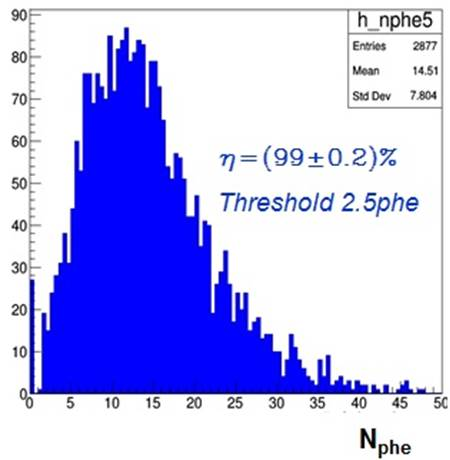
\includegraphics[width=1.0\linewidth,trim={0.0cm 0.0cm 0.0cm 0.0cm},clip]{images/RAFO_2GeV.jpg}
    \caption{Electron detection efficiency for elastically scattered electrons at 2 GeV. Data are obtained with the random trigger not correlated with the HTCC or other detector components of CLAS12.}
    \label{fig:RAFO_2GeV}
\end{figure}

Fig.~\ref{fig:positivePNPEC6595} shows the response of the detector in a wide range of particle momentum. The increase of number of events at high momenta is due to registration of charged pions (above threshold of their registration in the HTCC) and this is clearly illustrated.

\begin{figure}[!ht]
    \centering
    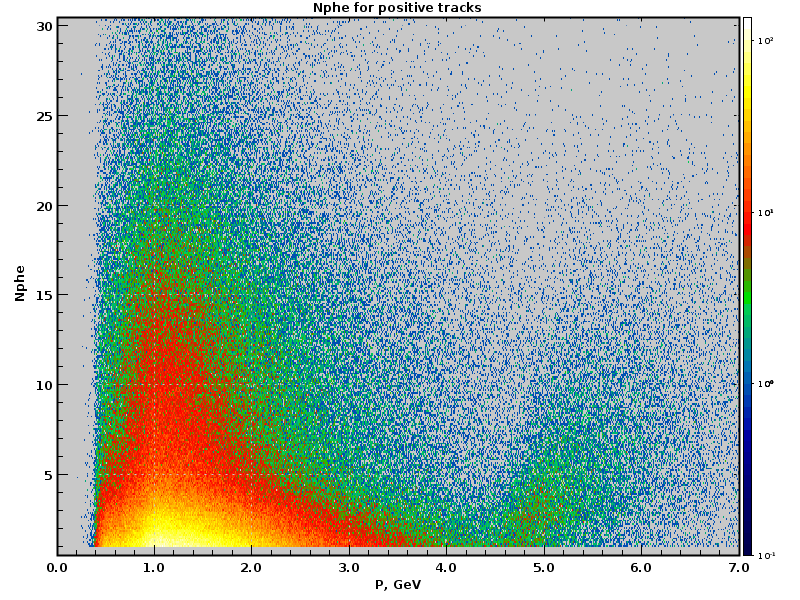
\includegraphics[width=1.0\linewidth,trim={0.0cm 0.0cm 0.0cm 0.0cm},clip]{images/positivePNPEC6595.png}
    \caption{Distributions of the HTCC response in a wide momentum range, including the region beyond the threshold of charged pion registration. Data obtained for positrons and $\pi^{+}$-mesons.}
    \label{fig:positivePNPEC6595}
\end{figure}

\begin{comment}
As shown bellow in the Fig.~\ref{fig:avgNPE_Theta_Phi_Dev_Build-2_NO_HOLES} the signal strength goes up for the utmost mirrors (large electron scattering angles). This is because electrons travel a longer distance in the radiator gas (10\% to 30\% difference depending on angle.) In other words the electron detection efficiency obtained for elastically scattered electrons at 2 GeV can be considered as as a conservative estimate for the efficiency of electron detection at larger angles.
\end{comment} 

The signal strength in the HTCC depends on the actual properties of the mirror facets, such as their final shape and reflectance. The accuracy of the combined mirror assembly and the alignment of the HTCC components (mirror, PMTs, Winston Cones), and the composition of the radiator gas all influence the final results. The FADC histogram of  the typical signal strength distribution obtained in one half-sector \#1 and \#2 of Sector 1 is shown in Fig.~\ref{fig:Signal_S1_HS1_HS2_R1_R2}. The signal strength for scattered electrons averaged over all HTCC channels is shown in Fig.~\ref{fig:Average_HTCC_Signal}. The experimentally measured mean value of 16.3 phe is close to Monte-Carlo simulation results, (see Fig.~\ref{fig:10cm_Targ_5T_Field_Phi}).

\begin{figure}[!ht]
    \centering
    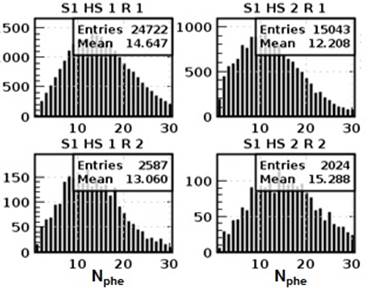
\includegraphics[width=1.0\linewidth,trim={0.0cm 0.0cm 0.0cm 0.0cm},clip]{images/Signal_S1_HS1_HS2_R1_R2.jpg}
    \caption{Typical distributions of the signal strength in channels covering polar angles in the range of $5^\circ$ to $12.5^\circ$ (Ring 1) and $12.5^\circ$ to $20.0^\circ$ (Ring 2) within azimuthal interval of $60^\circ$.}
    \label{fig:Signal_S1_HS1_HS2_R1_R2}
\end{figure}

\begin{figure}[!ht]
    \centering
    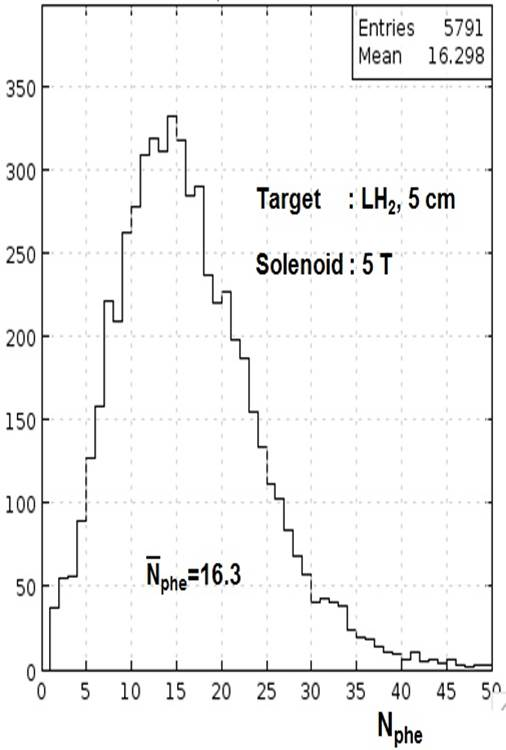
\includegraphics[width=1.0\linewidth,trim={0.0cm 0.0cm 0.0cm 0.0cm},clip]{images/Average_HTCC_Signal.jpg}
    \caption{The HTCC average signal strength for electrons from beam data.}
    \label{fig:Average_HTCC_Signal}
\end{figure}

Fig.~\ref{fig:HTCC_Response_run4013} shows the HTCC response for different electron momenta. Fig.~\ref{fig:avgNPE_Theta_Phi_Dev_Build-2_NO_HOLES}  shows the distribution of the HTCC response over the entire face of the mirror in the $x-y$-plane. Similar distribution is shown in Fig.~\ref{fig:avgNPE_XY_Dev_Build_02npe} obtained at the lower electron detection threshold of 0.2 photoelectrons. At the large electron scattering angles in range of 27.5$^\circ$ to 35$^\circ$, the statistics is lower. Fig.~\ref{fig:statistics_Theta_Phi_Dev_Build_NO_HOLES} shows the distribution of statistics in all 6 sectors. The data shows that the integrated signal strength is about 16.5 photoelectrons.

\begin{figure}[!ht]
    \centering
    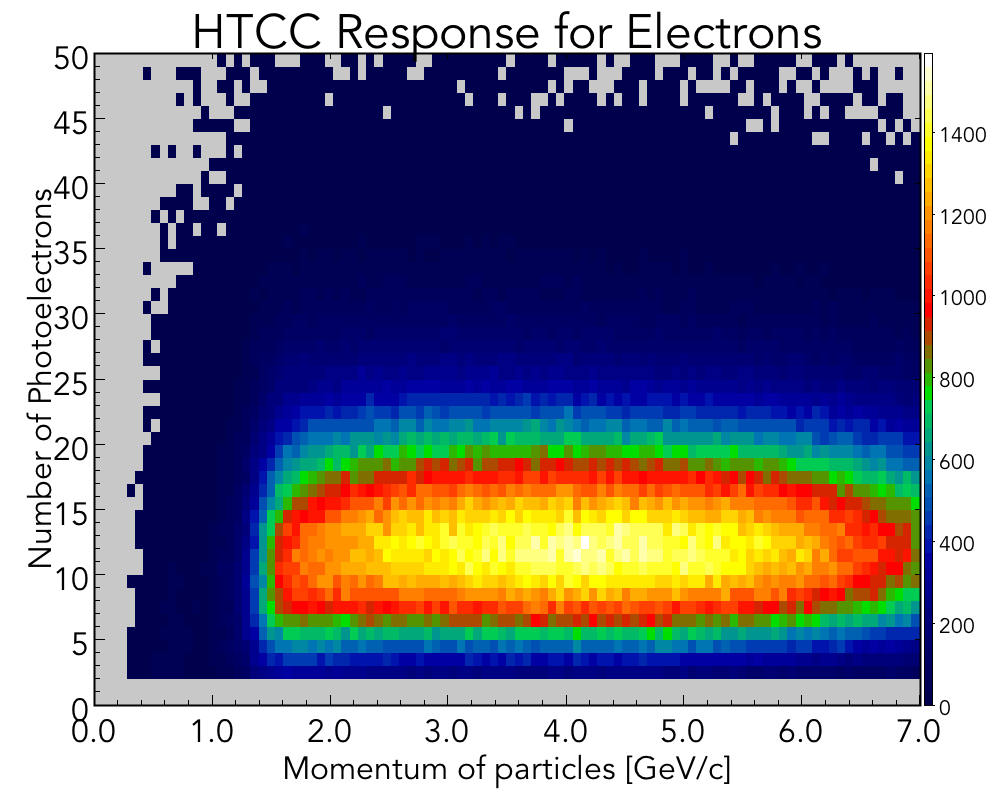
\includegraphics[width=1.0\linewidth,trim={0.0cm 0.0cm 0.0cm 1.73cm},clip]{images/HTCC_Response_run4013.png}
    \caption{The HTCC response for electrons: signal strength vs. momentum at 10.6 GeV energy.}
    \label{fig:HTCC_Response_run4013}
\end{figure}

\begin{figure}[!ht]
    \centering
    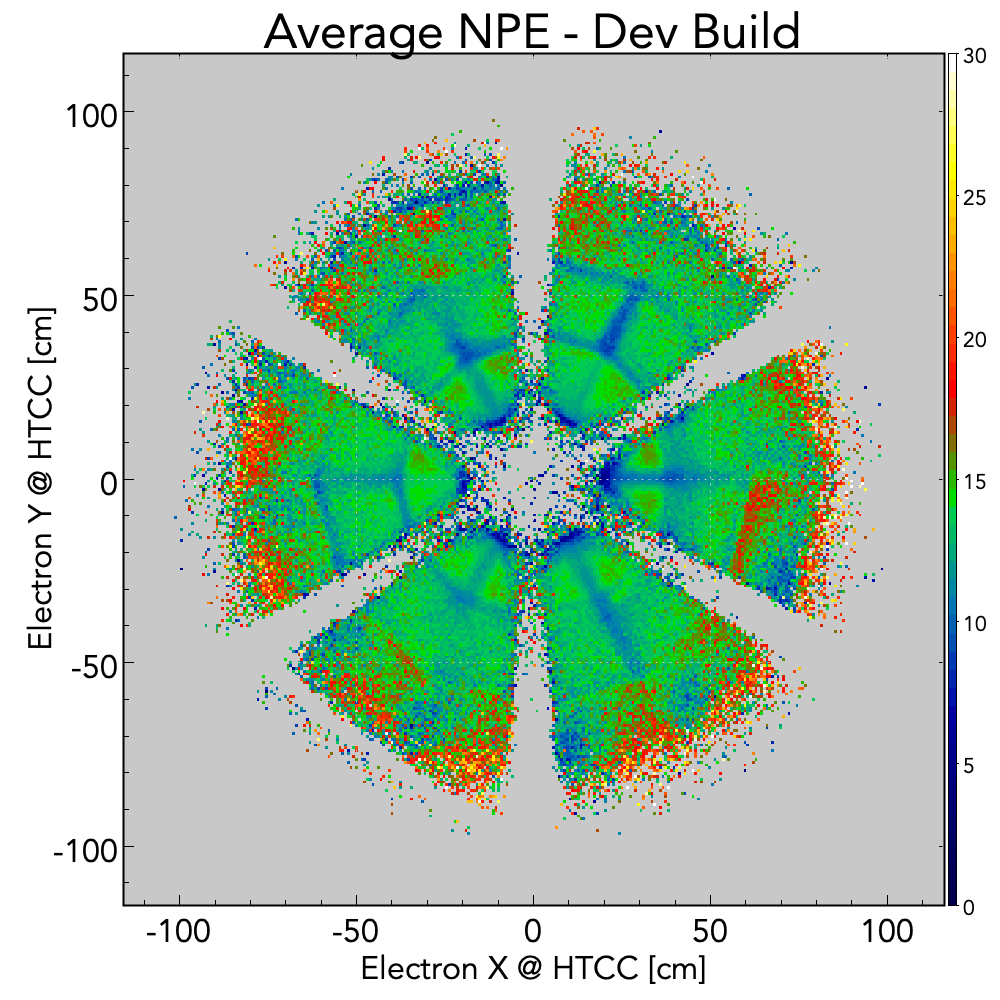
\includegraphics[width=1.0\linewidth,trim={0.0cm 0.0cm 0.0cm 1.67cm},clip]{images/avgNPE_Theta_Phi_Dev_Build-2_NO_HOLES.png}
    \caption{The HTCC response (in $N_{phe}$) for electrons in $x-y$-plane of the mirror.}
    \label{fig:avgNPE_Theta_Phi_Dev_Build-2_NO_HOLES}
\end{figure}

\begin{figure}[!ht]
    \centering
    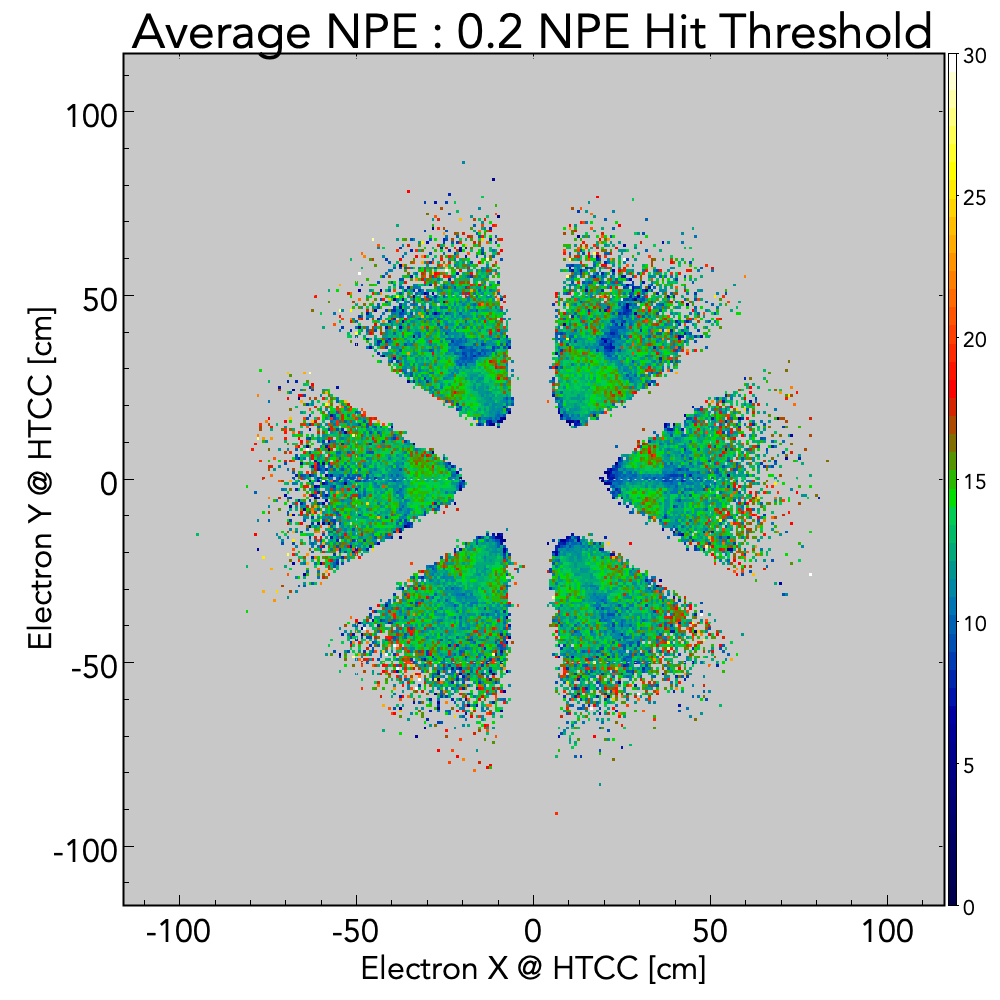
\includegraphics[width=1.0\linewidth,trim={0.0cm 0.0cm 0.0cm 1.67cm},clip]{images/avgNPE_XY_Dev_Build_02npe.png}
    \caption{The HTCC response (in $N_{phe}$) for electrons in $x-y$-plane of the mirror at the electron detection threshold of 0.2 photoelectrons.}
    \label{fig:avgNPE_XY_Dev_Build_02npe}
\end{figure}

\begin{figure}[!ht]
    \centering
    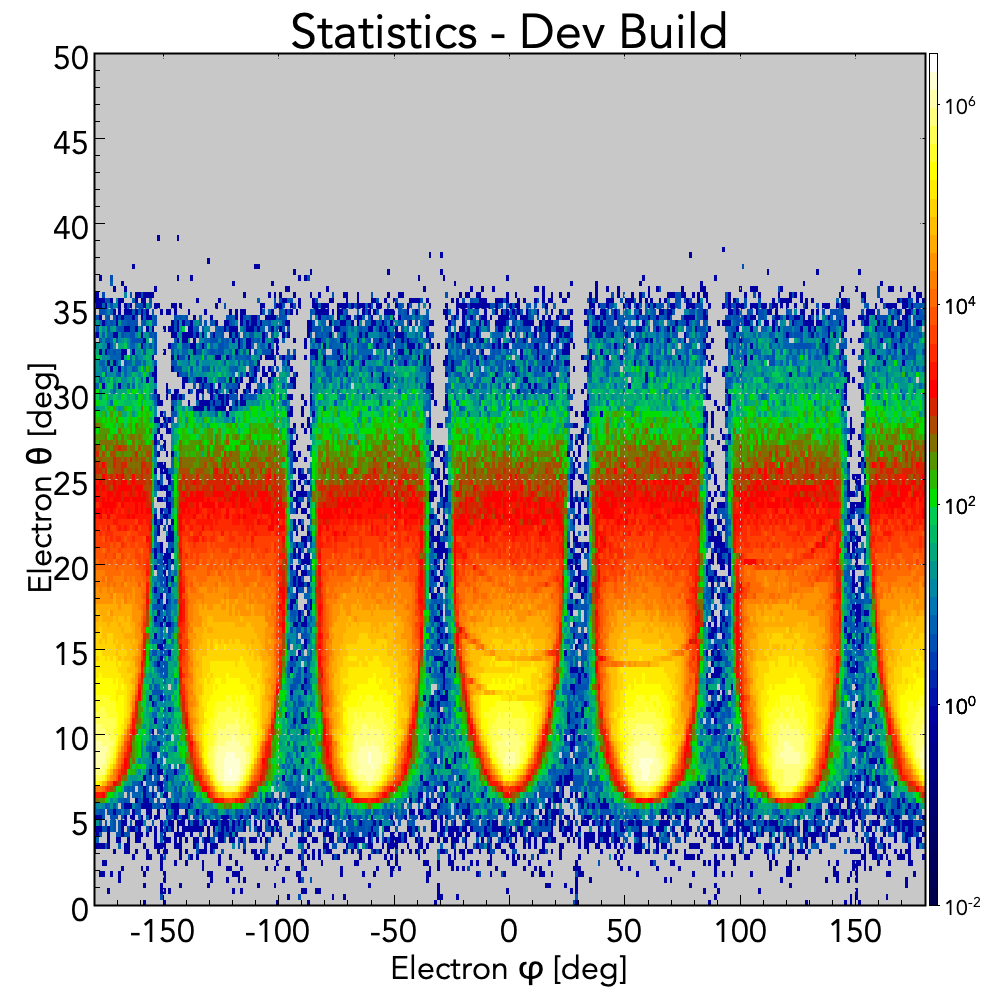
\includegraphics[width=1.0\linewidth,trim={0.0cm 0.0cm 0.0cm 1.67cm},clip]{images/statistics_Theta_Phi_Dev_Build_NO_HOLES.png}
    \caption{Distribution of statistics in all 6 sectors.}
    \label{fig:statistics_Theta_Phi_Dev_Build_NO_HOLES}
\end{figure}

We also note that in cases when the electrons cross the mirror close to its edges (at approximately at 5$^\circ$ and 35$^\circ$) one should expect unavoidable losses in the signal strength: some part of the Cherenkov light just passes by the mirror. As far as the internal borders between adjacent mirrors are concerned, there are similar losses that take place and are finally partially compensated due to the complete azimuthal symmetry of the detector, see Fig.~\ref{fig:avgNPE_Theta_Phi_Dev_Build-2_NO_HOLES}. The width of that area along internal boundaries that is deformed in the direction normal to the mirror face due to the shrinkage of the glue is estimated between $\sim$5 to $\sim$10 mm. This area includes the technological zone ~0.5 mm of width that is not reflecting the light at all. As a result these regions (width up to $\sim$10 mm) along internal boundaries between mirror facets defuse the light impinging the area, and therefore the signal strength is reduced. this edge effect is normal for the given design of the detector.


\section{Distribution and Documentation}


The gemc framework is documented on the gemc website \cite{gemc}. This includes the latest news and releases,
examples, procedure details and all options documentation.

The software is distributed in two ways: by downloading the source from the its public repository, or by using docker.

\subsubsection{Source Code Dowload}

The code repository is \url{https://github.com/gemc/source}. To compile GEMC several libraries are needed:


\begin{itemize}
	\item clhep: Class Library for High Energy Physics \cite{clhep}
	\item xercesc: validating XML parser \cite{xercesc}
	\item geant4: the libraries to simulate the passage of particles through matter \cite{geant4}
	\item qt: a C++ graphic library \cite{qt}
	\item evio: the CLAS12 data format \cite{evio}
	\item CCDB: the calibration database based on mysql 
\end{itemize}


\subsubsection{Docker}



repository code handling (fork and pull)

\subsection{clas12tags} 





\section{Acknowledgements}

We appreciate the contribution of J.  Andresen, C. Britton, S. Chappa, A. Dyer, J. Hoff, V. Re, and T. Zimmerman to the design of the HFCB. We are grateful to administrative, engineering, and technical staff of Fermilab Silicon Detector Facility for excellent work on module assembly.

\section{Conclusions}

The SVT is installed in the CLAS experimental hall, performance of modules measured during detector integration has been confirmed. No channels were lost during the installation. SVT barrel has been electrically  tested with number of defective channels 0.1$\%$, well within the specification. The chip average ENC noise is uniform $\sim$1600 e in normal operating conditions. There is no evidence of coherent noise between the modules and other components. The tracker has been commissioned with cosmic rays and integrated as part of  CLAS central detector. Tracking performance was confirmed with beam data and matches physics requirements. 





\section{References}

\bibliography{bibfile}
\bibliographystyle{elsarticle-num}

\end{document}








